\documentclass[acmlarge]{acmart}\settopmatter{printfolios=true}
% Uncomment the line below to blind for reviewing (will rm acknowledgements):
% \documentclass[acmlarge,review,anonymous]{acmart}\settopmatter{printfolios=true}

\usepackage[utf8]{inputenc}
% the following standard packages may be helpful, but are not required
%\usepackage{longtable}
\usepackage{mathtools}
\usepackage{multicol}
\usepackage{multirow}
\usepackage{booktabs}
\usepackage{courier}
\usepackage[scaled]{helvet}
\usepackage{listings}
\usepackage{enumitem}
\usepackage{mdwlist} % tighter description environment (starred)
\usepackage{gensymb}
\usepackage{hyperref}
\usepackage{caption}
\usepackage{fp}

\usepackage{graphicx}
\usepackage{softdev}
\usepackage{amsmath}
\usepackage{mdwlist}
\usepackage{pifont}
\usepackage{xspace}

\usepackage{sparklines}

\newcommand{\kalibera}{Kalibera \& Jones\xspace}
\newcommand{\krun}{Krun\xspace}
\newcommand{\hypone}{H1\xspace}
\newcommand{\hyptwo}{H2\xspace}
\newcommand{\binarytrees}{\emph{binary trees}\xspace}
\newcommand{\richards}{\emph{Richards}\xspace}
\newcommand{\spectralnorm}{\emph{spectralnorm}\xspace}
\newcommand{\nbody}{\emph{n-body}\xspace}
\newcommand{\fasta}{\emph{fasta}\xspace}
\newcommand{\fannkuch}{\emph{fannkuch redux}\xspace}
\newcommand{\bencherthree}{Linux$_\mathrm{4790K}$\xspace}
\newcommand{\bencherfive}{Linux$_\mathrm{4790}$\xspace}
\newcommand{\benchersix}{OpenBSD$_\mathrm{4790}$\xspace}
\newcommand{\bencherseven}{Linux$_\mathrm{E3-1240v5}$\xspace}

\DeclareRobustCommand{\flatc}{%
\setlength{\sparklinethickness}{0.4pt}%
\begin{sparkline}{1.5}
\spark 0.1 0.35
       0.9 0.35
       /%
\end{sparkline}\xspace}
\DeclareRobustCommand{\nosteadystate}{%
\setlength{\sparklinethickness}{0.4pt}%
\begin{sparkline}{1.5}
\spark 0.1 0.2
       0.26 0.5
       0.42 0.2
       0.58 0.5
       0.74 0.2
       0.90 0.5
       /%
\end{sparkline}\xspace}
\DeclareRobustCommand{\warmup}{%
\setlength{\sparklinethickness}{0.4pt}%
\begin{sparkline}{1.5}
\spark 0.1 0.8
       0.5 0.8
       0.5 0.0
       0.9 0.0
       /%
\end{sparkline}\xspace}
\DeclareRobustCommand{\slowdown}{%
\setlength{\sparklinethickness}{0.4pt}%
\begin{sparkline}{1.5}
\spark 0.1 0.0
       0.5 0.0
       0.5 0.8
       0.9 0.8
       /%
\end{sparkline}\xspace}
\DeclareRobustCommand{\inconsistent}{%
\setlength{\sparklinethickness}{0.4pt}%
\begin{sparkline}{1.5}
\spark 0.1 0.4
       0.9 0.4
       /%
\spark 0.1 0.2
       0.9 0.2
       /%
\spark 0.1 0.6
       0.9 0.0
       /%
\end{sparkline}\xspace}
\DeclareRobustCommand{\goodinconsistent}{%
\setlength{\sparklinethickness}{0.4pt}%
\begin{sparkline}{1.5}
\spark 0.1 0.4
       0.9 0.4
       /%
\spark 0.1 0.2
       0.9 0.2
       /%
\spark 0.2 0.3
       0.4 0.0
       0.8 0.6
       /%
\end{sparkline}\xspace}
\DeclareRobustCommand{\badinconsistent}{%
\setlength{\sparklinethickness}{0.4pt}%
\begin{sparkline}{1.5}
\spark 0.1 0.4
       0.9 0.4
       /%
\spark 0.1 0.2
       0.9 0.2
       /%
\spark 0.3 0.6
       0.7 0.0
       /%
\spark 0.3 0.0
       0.7 0.6
       /%
\end{sparkline}\xspace}

%%%
%%% Total outliers and percentages over all executions.
%%%
\newcommand{\totaloutliers}{8676}
\newcommand{\totaloutlierspercentage}{0.4}
%%%
%%% Maximum outliers for one process execution.
%%%
\newcommand{\maximumoutliers}{133}
%%%
%%% Outliers per machine.
%%%
%%% bencher3.
\newcommand{\bencherthreeoutliers}{4114}
\newcommand{\bencherthreeoutlierspercentage}{0.4}
%%% bencher5.
\newcommand{\bencherfiveoutliers}{2336}
\newcommand{\bencherfiveoutlierspercentage}{0.3}
%%% bencher6.
\newcommand{\benchersixoutliers}{2226}
\newcommand{\benchersixoutlierspercentage}{0.4}
%%%
%%% Classifications per vm/benchmark pair.
%%%
%%% Hotspot nbody.
\newcommand{\hotspotnbodyoutliers}{8}
\newcommand{\hotspotnbodyoutlierspercentage}{0.0}
%%% LuaJIT richards.
\newcommand{\luajitrichardsoutliers}{8}
\newcommand{\luajitrichardsoutlierspercentage}{0.0}
%%% Graal fasta.
\newcommand{\graalfastaoutliers}{2}
\newcommand{\graalfastaoutlierspercentage}{0.0}
%%% PyPy nbody.
\newcommand{\pypynbodyoutliers}{2}
\newcommand{\pypynbodyoutlierspercentage}{0.0}
%%% LuaJIT binarytrees.
\newcommand{\luajitbinarytreesoutliers}{1676}
\newcommand{\luajitbinarytreesoutlierspercentage}{2.8}
%%% Graal fannkuch_redux.
\newcommand{\graalfannkuchreduxoutliers}{29}
\newcommand{\graalfannkuchreduxoutlierspercentage}{0.1}
%%% JRubyTruffle binarytrees.
\newcommand{\jrubytrufflebinarytreesoutliers}{133}
\newcommand{\jrubytrufflebinarytreesoutlierspercentage}{0.3}
%%% V8 nbody.
\newcommand{\veightnbodyoutliers}{54}
\newcommand{\veightnbodyoutlierspercentage}{0.1}
%%% JRubyTruffle nbody.
\newcommand{\jrubytrufflenbodyoutliers}{181}
\newcommand{\jrubytrufflenbodyoutlierspercentage}{0.5}
%%% V8 richards.
\newcommand{\veightrichardsoutliers}{19}
\newcommand{\veightrichardsoutlierspercentage}{0.0}
%%% Hotspot fasta.
\newcommand{\hotspotfastaoutliers}{14}
\newcommand{\hotspotfastaoutlierspercentage}{0.0}
%%% V8 binarytrees.
\newcommand{\veightbinarytreesoutliers}{2}
\newcommand{\veightbinarytreesoutlierspercentage}{0.0}
%%% PyPy fannkuch_redux.
\newcommand{\pypyfannkuchreduxoutliers}{67}
\newcommand{\pypyfannkuchreduxoutlierspercentage}{0.1}
%%% V8 fannkuch_redux.
\newcommand{\veightfannkuchreduxoutliers}{427}
\newcommand{\veightfannkuchreduxoutlierspercentage}{0.7}
%%% C richards.
\newcommand{\crichardsoutliers}{260}
\newcommand{\crichardsoutlierspercentage}{0.4}
%%% HHVM fannkuch_redux.
\newcommand{\hhvmfannkuchreduxoutliers}{80}
\newcommand{\hhvmfannkuchreduxoutlierspercentage}{0.2}
%%% V8 fasta.
\newcommand{\veightfastaoutliers}{1}
\newcommand{\veightfastaoutlierspercentage}{0.0}
%%% V8 spectralnorm.
\newcommand{\veightspectralnormoutliers}{198}
\newcommand{\veightspectralnormoutlierspercentage}{0.3}
%%% Graal nbody.
\newcommand{\graalnbodyoutliers}{9}
\newcommand{\graalnbodyoutlierspercentage}{0.0}
%%% Hotspot fannkuch_redux.
\newcommand{\hotspotfannkuchreduxoutliers}{6}
\newcommand{\hotspotfannkuchreduxoutlierspercentage}{0.0}
%%% C binarytrees.
\newcommand{\cbinarytreesoutliers}{61}
\newcommand{\cbinarytreesoutlierspercentage}{0.1}
%%% HHVM binarytrees.
\newcommand{\hhvmbinarytreesoutliers}{38}
\newcommand{\hhvmbinarytreesoutlierspercentage}{0.1}
%%% HHVM fasta.
\newcommand{\hhvmfastaoutliers}{93}
\newcommand{\hhvmfastaoutlierspercentage}{0.2}
%%% PyPy binarytrees.
\newcommand{\pypybinarytreesoutliers}{52}
\newcommand{\pypybinarytreesoutlierspercentage}{0.1}
%%% Graal richards.
\newcommand{\graalrichardsoutliers}{509}
\newcommand{\graalrichardsoutlierspercentage}{1.3}
%%% C fannkuch_redux.
\newcommand{\cfannkuchreduxoutliers}{3}
\newcommand{\cfannkuchreduxoutlierspercentage}{0.0}
%%% PyPy spectralnorm.
\newcommand{\pypyspectralnormoutliers}{1010}
\newcommand{\pypyspectralnormoutlierspercentage}{1.7}
%%% HHVM spectralnorm.
\newcommand{\hhvmspectralnormoutliers}{46}
\newcommand{\hhvmspectralnormoutlierspercentage}{0.1}
%%% JRubyTruffle fannkuch_redux.
\newcommand{\jrubytrufflefannkuchreduxoutliers}{49}
\newcommand{\jrubytrufflefannkuchreduxoutlierspercentage}{0.1}
%%% Hotspot richards.
\newcommand{\hotspotrichardsoutliers}{52}
\newcommand{\hotspotrichardsoutlierspercentage}{0.1}
%%% LuaJIT spectralnorm.
\newcommand{\luajitspectralnormoutliers}{5}
\newcommand{\luajitspectralnormoutlierspercentage}{0.0}
%%% PyPy richards.
\newcommand{\pypyrichardsoutliers}{1483}
\newcommand{\pypyrichardsoutlierspercentage}{2.5}
%%% LuaJIT fasta.
\newcommand{\luajitfastaoutliers}{3}
\newcommand{\luajitfastaoutlierspercentage}{0.0}
%%% Graal spectralnorm.
\newcommand{\graalspectralnormoutliers}{241}
\newcommand{\graalspectralnormoutlierspercentage}{0.6}
%%% HHVM nbody.
\newcommand{\hhvmnbodyoutliers}{447}
\newcommand{\hhvmnbodyoutlierspercentage}{1.1}
%%% JRubyTruffle richards.
\newcommand{\jrubytrufflerichardsoutliers}{88}
\newcommand{\jrubytrufflerichardsoutlierspercentage}{0.2}
%%% LuaJIT fannkuch_redux.
\newcommand{\luajitfannkuchreduxoutliers}{1}
\newcommand{\luajitfannkuchreduxoutlierspercentage}{0.0}
%%% Hotspot binarytrees.
\newcommand{\hotspotbinarytreesoutliers}{7}
\newcommand{\hotspotbinarytreesoutlierspercentage}{0.0}
%%% JRubyTruffle spectralnorm.
\newcommand{\jrubytrufflespectralnormoutliers}{124}
\newcommand{\jrubytrufflespectralnormoutlierspercentage}{0.3}
%%% C spectralnorm.
\newcommand{\cspectralnormoutliers}{15}
\newcommand{\cspectralnormoutlierspercentage}{0.0}
%%% Graal binarytrees.
\newcommand{\graalbinarytreesoutliers}{2}
\newcommand{\graalbinarytreesoutlierspercentage}{0.0}
%%% LuaJIT nbody.
\newcommand{\luajitnbodyoutliers}{132}
\newcommand{\luajitnbodyoutlierspercentage}{0.2}
%%% C fasta.
\newcommand{\cfastaoutliers}{176}
\newcommand{\cfastaoutlierspercentage}{0.3}
%%% C nbody.
\newcommand{\cnbodyoutliers}{615}
\newcommand{\cnbodyoutlierspercentage}{1.0}
%%% Hotspot spectralnorm.
\newcommand{\hotspotspectralnormoutliers}{233}
\newcommand{\hotspotspectralnormoutlierspercentage}{0.4}
%%% PyPy fasta.
\newcommand{\pypyfastaoutliers}{15}
\newcommand{\pypyfastaoutlierspercentage}{0.0}

%%%
%%% Total executions and iterations.
%%%
\newcommand{\totalpexecs}{3660}
\newcommand{\totaliterations}{7320000}
\newcommand{\bencherfivetotalpexecs}{1380}
\newcommand{\benchersixtotalpexecs}{900}
\newcommand{\bencherseventotalpexecs}{1380}
\newcommand{\bencherfivetotaliterations}{2760000}
\newcommand{\benchersixtotaliterations}{1800000}
\newcommand{\bencherseventotaliterations}{2760000}
%%%
%%% Total classifications over all executions.
%%%
\newcommand{\totalflat}{959}
\newcommand{\totalnosteadystate}{278}
\newcommand{\totalslowdown}{577}
\newcommand{\totalwarmup}{1846}
%%%
%%% Percentage classifications over all executions.
%%%
\newcommand{\totalflatpercentage}{26.2}
\newcommand{\totalnosteadystatepercentage}{7.6}
\newcommand{\totalslowdownpercentage}{15.8}
\newcommand{\totalwarmuppercentage}{50.4}
%%%
%%% Total consistent classifications over all executions.
%%%
\newcommand{\totalconsistent}{50}
\newcommand{\totalgoodinconsistent}{10}
\newcommand{\totalbadinconsistent}{62}
%%%
%%% Percentage consistent classifications over all executions.
%%%
\newcommand{\totalconsistentpercentage}{41.0}
\newcommand{\totalgoodinconsistentpercentage}{8.2}
\newcommand{\totalbadinconsistentpercentage}{50.8}
%%%
%%% Classifications per machine (machine category).
%%%
%%% bencher5.
\newcommand{\bencherfiveflat}{364}
\newcommand{\bencherfivenosteadystate}{120}
\newcommand{\bencherfiveslowdown}{230}
\newcommand{\bencherfivewarmup}{666}
%%% bencher7.
\newcommand{\benchersevenflat}{289}
\newcommand{\benchersevennosteadystate}{133}
\newcommand{\benchersevenslowdown}{247}
\newcommand{\benchersevenwarmup}{711}
%%% bencher6.
\newcommand{\benchersixflat}{306}
\newcommand{\benchersixnosteadystate}{25}
\newcommand{\benchersixslowdown}{100}
\newcommand{\benchersixwarmup}{469}
%%%
%%% Machine / classification percentages (machine category percentage).
%%%
%%% bencher5.
\newcommand{\bencherfiveflatpercentage}{26.4}
\newcommand{\bencherfivenosteadystatepercentage}{8.7}
\newcommand{\bencherfiveslowdownpercentage}{16.7}
\newcommand{\bencherfivewarmuppercentage}{48.3}
%%% bencher7.
\newcommand{\benchersevenflatpercentage}{20.9}
\newcommand{\benchersevennosteadystatepercentage}{9.6}
\newcommand{\benchersevenslowdownpercentage}{17.9}
\newcommand{\benchersevenwarmuppercentage}{51.5}
%%% bencher6.
\newcommand{\benchersixflatpercentage}{34.0}
\newcommand{\benchersixnosteadystatepercentage}{2.8}
\newcommand{\benchersixslowdownpercentage}{11.1}
\newcommand{\benchersixwarmuppercentage}{52.1}
%%%
%%% Classifications per machine / vm/bench pair (machine vmbench category).
%%%
%%% bencher5.
\newcommand{\bencherfivevmbenchpairsbadinconsistent}{21}
\newcommand{\bencherfivevmbenchpairsflat}{4}
\newcommand{\bencherfivevmbenchpairsgoodinconsistent}{3}
\newcommand{\bencherfivevmbenchpairsnosteadystate}{2}
\newcommand{\bencherfivevmbenchpairsslowdown}{3}
\newcommand{\bencherfivevmbenchpairswarmup}{13}
%%% bencher7.
\newcommand{\benchersevenvmbenchpairsbadinconsistent}{20}
\newcommand{\benchersevenvmbenchpairsflat}{6}
\newcommand{\benchersevenvmbenchpairsgoodinconsistent}{3}
\newcommand{\benchersevenvmbenchpairsnosteadystate}{3}
\newcommand{\benchersevenvmbenchpairsslowdown}{3}
\newcommand{\benchersevenvmbenchpairswarmup}{11}
%%% bencher6.
\newcommand{\benchersixvmbenchpairsbadinconsistent}{21}
\newcommand{\benchersixvmbenchpairsflat}{2}
\newcommand{\benchersixvmbenchpairsgoodinconsistent}{4}
\newcommand{\benchersixvmbenchpairsnosteadystate}{0}
\newcommand{\benchersixvmbenchpairsslowdown}{0}
\newcommand{\benchersixvmbenchpairswarmup}{3}
%%%
%%% Machine / vm/bench classification percentages (machine vmbench category percentage).
%%%
%%% bencher5.
\newcommand{\bencherfivevmbenchpairsbadinconsistentpercentage}{45.7}
\newcommand{\bencherfivevmbenchpairsflatpercentage}{8.7}
\newcommand{\bencherfivevmbenchpairsgoodinconsistentpercentage}{6.5}
\newcommand{\bencherfivevmbenchpairsnosteadystatepercentage}{4.3}
\newcommand{\bencherfivevmbenchpairsslowdownpercentage}{6.5}
\newcommand{\bencherfivevmbenchpairswarmuppercentage}{28.3}
%%% bencher7.
\newcommand{\benchersevenvmbenchpairsbadinconsistentpercentage}{43.5}
\newcommand{\benchersevenvmbenchpairsflatpercentage}{13.0}
\newcommand{\benchersevenvmbenchpairsgoodinconsistentpercentage}{6.5}
\newcommand{\benchersevenvmbenchpairsnosteadystatepercentage}{6.5}
\newcommand{\benchersevenvmbenchpairsslowdownpercentage}{6.5}
\newcommand{\benchersevenvmbenchpairswarmuppercentage}{23.9}
%%% bencher6.
\newcommand{\benchersixvmbenchpairsbadinconsistentpercentage}{70.0}
\newcommand{\benchersixvmbenchpairsflatpercentage}{6.7}
\newcommand{\benchersixvmbenchpairsgoodinconsistentpercentage}{13.3}
\newcommand{\benchersixvmbenchpairsnosteadystatepercentage}{0.0}
\newcommand{\benchersixvmbenchpairsslowdownpercentage}{0.0}
\newcommand{\benchersixvmbenchpairswarmuppercentage}{10.0}
%%%
%%% Consistent classifications per machine (machine consistent).
%%%
%%% bencher5.
\newcommand{\bencherfiveconsistent}{22}
\newcommand{\bencherfivegoodinconsistent}{3}
\newcommand{\bencherfivebadinconsistent}{21}
%%% bencher7.
\newcommand{\benchersevenconsistent}{23}
\newcommand{\benchersevengoodinconsistent}{3}
\newcommand{\benchersevenbadinconsistent}{20}
%%% bencher6.
\newcommand{\benchersixconsistent}{5}
\newcommand{\benchersixgoodinconsistent}{4}
\newcommand{\benchersixbadinconsistent}{21}
%%%
%%% Consistent machine percentages (machine consistent percentage).
%%%
%%% bencher5.
\newcommand{\bencherfiveconsistentpercentage}{47.8}
\newcommand{\bencherfivegoodinconsistentpercentage}{6.5}
\newcommand{\bencherfivebadinconsistentpercentage}{45.7}
%%% bencher7.
\newcommand{\benchersevenconsistentpercentage}{50.0}
\newcommand{\benchersevengoodinconsistentpercentage}{6.5}
\newcommand{\benchersevenbadinconsistentpercentage}{43.5}
%%% bencher6.
\newcommand{\benchersixconsistentpercentage}{16.7}
\newcommand{\benchersixgoodinconsistentpercentage}{13.3}
\newcommand{\benchersixbadinconsistentpercentage}{70.0}
%%%
%%% Classifications per vm/benchmark pair (VM bmark category).
%%%
%%% Hotspot nbody.
\newcommand{\hotspotnbodyflat}{0}
\newcommand{\hotspotnbodynosteadystate}{0}
\newcommand{\hotspotnbodyslowdown}{0}
\newcommand{\hotspotnbodywarmup}{90}
%%% LuaJIT richards.
\newcommand{\luajitrichardsflat}{28}
\newcommand{\luajitrichardsnosteadystate}{22}
\newcommand{\luajitrichardsslowdown}{8}
\newcommand{\luajitrichardswarmup}{32}
%%% Graal fasta.
\newcommand{\graalfastaflat}{0}
\newcommand{\graalfastanosteadystate}{1}
\newcommand{\graalfastaslowdown}{0}
\newcommand{\graalfastawarmup}{59}
%%% PyPy nbody.
\newcommand{\pypynbodyflat}{85}
\newcommand{\pypynbodynosteadystate}{0}
\newcommand{\pypynbodyslowdown}{1}
\newcommand{\pypynbodywarmup}{4}
%%% LuaJIT binarytrees.
\newcommand{\luajitbinarytreesflat}{30}
\newcommand{\luajitbinarytreesnosteadystate}{8}
\newcommand{\luajitbinarytreesslowdown}{8}
\newcommand{\luajitbinarytreeswarmup}{44}
%%% Graal fannkuch_redux.
\newcommand{\graalfannkuchreduxflat}{0}
\newcommand{\graalfannkuchreduxnosteadystate}{4}
\newcommand{\graalfannkuchreduxslowdown}{1}
\newcommand{\graalfannkuchreduxwarmup}{55}
%%% JRubyTruffle binarytrees.
\newcommand{\jrubytrufflebinarytreesflat}{0}
\newcommand{\jrubytrufflebinarytreesnosteadystate}{4}
\newcommand{\jrubytrufflebinarytreesslowdown}{37}
\newcommand{\jrubytrufflebinarytreeswarmup}{19}
%%% V8 nbody.
\newcommand{\veightnbodyflat}{65}
\newcommand{\veightnbodynosteadystate}{0}
\newcommand{\veightnbodyslowdown}{0}
\newcommand{\veightnbodywarmup}{25}
%%% JRubyTruffle nbody.
\newcommand{\jrubytrufflenbodyflat}{0}
\newcommand{\jrubytrufflenbodynosteadystate}{0}
\newcommand{\jrubytrufflenbodyslowdown}{0}
\newcommand{\jrubytrufflenbodywarmup}{60}
%%% V8 richards.
\newcommand{\veightrichardsflat}{1}
\newcommand{\veightrichardsnosteadystate}{0}
\newcommand{\veightrichardsslowdown}{6}
\newcommand{\veightrichardswarmup}{83}
%%% Hotspot fasta.
\newcommand{\hotspotfastaflat}{0}
\newcommand{\hotspotfastanosteadystate}{0}
\newcommand{\hotspotfastaslowdown}{23}
\newcommand{\hotspotfastawarmup}{67}
%%% V8 binarytrees.
\newcommand{\veightbinarytreesflat}{17}
\newcommand{\veightbinarytreesnosteadystate}{13}
\newcommand{\veightbinarytreesslowdown}{16}
\newcommand{\veightbinarytreeswarmup}{44}
%%% PyPy fannkuch_redux.
\newcommand{\pypyfannkuchreduxflat}{16}
\newcommand{\pypyfannkuchreduxnosteadystate}{0}
\newcommand{\pypyfannkuchreduxslowdown}{2}
\newcommand{\pypyfannkuchreduxwarmup}{72}
%%% V8 fannkuch_redux.
\newcommand{\veightfannkuchreduxflat}{60}
\newcommand{\veightfannkuchreduxnosteadystate}{0}
\newcommand{\veightfannkuchreduxslowdown}{0}
\newcommand{\veightfannkuchreduxwarmup}{30}
%%% C richards.
\newcommand{\crichardsflat}{63}
\newcommand{\crichardsnosteadystate}{6}
\newcommand{\crichardsslowdown}{10}
\newcommand{\crichardswarmup}{11}
%%% HHVM fannkuch_redux.
\newcommand{\hhvmfannkuchreduxflat}{0}
\newcommand{\hhvmfannkuchreduxnosteadystate}{0}
\newcommand{\hhvmfannkuchreduxslowdown}{1}
\newcommand{\hhvmfannkuchreduxwarmup}{59}
%%% V8 fasta.
\newcommand{\veightfastaflat}{0}
\newcommand{\veightfastanosteadystate}{1}
\newcommand{\veightfastaslowdown}{55}
\newcommand{\veightfastawarmup}{34}
%%% V8 spectralnorm.
\newcommand{\veightspectralnormflat}{1}
\newcommand{\veightspectralnormnosteadystate}{0}
\newcommand{\veightspectralnormslowdown}{0}
\newcommand{\veightspectralnormwarmup}{89}
%%% Graal nbody.
\newcommand{\graalnbodyflat}{0}
\newcommand{\graalnbodynosteadystate}{0}
\newcommand{\graalnbodyslowdown}{0}
\newcommand{\graalnbodywarmup}{60}
%%% Hotspot fannkuch_redux.
\newcommand{\hotspotfannkuchreduxflat}{0}
\newcommand{\hotspotfannkuchreduxnosteadystate}{19}
\newcommand{\hotspotfannkuchreduxslowdown}{3}
\newcommand{\hotspotfannkuchreduxwarmup}{68}
%%% C binarytrees.
\newcommand{\cbinarytreesflat}{30}
\newcommand{\cbinarytreesnosteadystate}{60}
\newcommand{\cbinarytreesslowdown}{0}
\newcommand{\cbinarytreeswarmup}{0}
%%% HHVM binarytrees.
\newcommand{\hhvmbinarytreesflat}{0}
\newcommand{\hhvmbinarytreesnosteadystate}{6}
\newcommand{\hhvmbinarytreesslowdown}{12}
\newcommand{\hhvmbinarytreeswarmup}{42}
%%% HHVM fasta.
\newcommand{\hhvmfastaflat}{0}
\newcommand{\hhvmfastanosteadystate}{2}
\newcommand{\hhvmfastaslowdown}{1}
\newcommand{\hhvmfastawarmup}{57}
%%% PyPy binarytrees.
\newcommand{\pypybinarytreesflat}{8}
\newcommand{\pypybinarytreesnosteadystate}{14}
\newcommand{\pypybinarytreesslowdown}{47}
\newcommand{\pypybinarytreeswarmup}{21}
%%% Graal richards.
\newcommand{\graalrichardsflat}{0}
\newcommand{\graalrichardsnosteadystate}{1}
\newcommand{\graalrichardsslowdown}{2}
\newcommand{\graalrichardswarmup}{57}
%%% C fannkuch_redux.
\newcommand{\cfannkuchreduxflat}{68}
\newcommand{\cfannkuchreduxnosteadystate}{2}
\newcommand{\cfannkuchreduxslowdown}{3}
\newcommand{\cfannkuchreduxwarmup}{17}
%%% PyPy spectralnorm.
\newcommand{\pypyspectralnormflat}{0}
\newcommand{\pypyspectralnormnosteadystate}{0}
\newcommand{\pypyspectralnormslowdown}{2}
\newcommand{\pypyspectralnormwarmup}{88}
%%% HHVM spectralnorm.
\newcommand{\hhvmspectralnormflat}{0}
\newcommand{\hhvmspectralnormnosteadystate}{0}
\newcommand{\hhvmspectralnormslowdown}{0}
\newcommand{\hhvmspectralnormwarmup}{60}
%%% JRubyTruffle fannkuch_redux.
\newcommand{\jrubytrufflefannkuchreduxflat}{0}
\newcommand{\jrubytrufflefannkuchreduxnosteadystate}{0}
\newcommand{\jrubytrufflefannkuchreduxslowdown}{60}
\newcommand{\jrubytrufflefannkuchreduxwarmup}{0}
%%% Hotspot richards.
\newcommand{\hotspotrichardsflat}{0}
\newcommand{\hotspotrichardsnosteadystate}{5}
\newcommand{\hotspotrichardsslowdown}{83}
\newcommand{\hotspotrichardswarmup}{2}
%%% LuaJIT spectralnorm.
\newcommand{\luajitspectralnormflat}{83}
\newcommand{\luajitspectralnormnosteadystate}{0}
\newcommand{\luajitspectralnormslowdown}{2}
\newcommand{\luajitspectralnormwarmup}{5}
%%% PyPy richards.
\newcommand{\pypyrichardsflat}{0}
\newcommand{\pypyrichardsnosteadystate}{0}
\newcommand{\pypyrichardsslowdown}{0}
\newcommand{\pypyrichardswarmup}{90}
%%% LuaJIT fasta.
\newcommand{\luajitfastaflat}{48}
\newcommand{\luajitfastanosteadystate}{31}
\newcommand{\luajitfastaslowdown}{1}
\newcommand{\luajitfastawarmup}{10}
%%% Graal spectralnorm.
\newcommand{\graalspectralnormflat}{10}
\newcommand{\graalspectralnormnosteadystate}{0}
\newcommand{\graalspectralnormslowdown}{50}
\newcommand{\graalspectralnormwarmup}{0}
%%% HHVM nbody.
\newcommand{\hhvmnbodyflat}{0}
\newcommand{\hhvmnbodynosteadystate}{3}
\newcommand{\hhvmnbodyslowdown}{11}
\newcommand{\hhvmnbodywarmup}{46}
%%% JRubyTruffle richards.
\newcommand{\jrubytrufflerichardsflat}{0}
\newcommand{\jrubytrufflerichardsnosteadystate}{0}
\newcommand{\jrubytrufflerichardsslowdown}{60}
\newcommand{\jrubytrufflerichardswarmup}{0}
%%% LuaJIT fannkuch_redux.
\newcommand{\luajitfannkuchreduxflat}{82}
\newcommand{\luajitfannkuchreduxnosteadystate}{1}
\newcommand{\luajitfannkuchreduxslowdown}{1}
\newcommand{\luajitfannkuchreduxwarmup}{6}
%%% Hotspot binarytrees.
\newcommand{\hotspotbinarytreesflat}{0}
\newcommand{\hotspotbinarytreesnosteadystate}{0}
\newcommand{\hotspotbinarytreesslowdown}{9}
\newcommand{\hotspotbinarytreeswarmup}{81}
%%% JRubyTruffle spectralnorm.
\newcommand{\jrubytrufflespectralnormflat}{0}
\newcommand{\jrubytrufflespectralnormnosteadystate}{0}
\newcommand{\jrubytrufflespectralnormslowdown}{2}
\newcommand{\jrubytrufflespectralnormwarmup}{58}
%%% C spectralnorm.
\newcommand{\cspectralnormflat}{18}
\newcommand{\cspectralnormnosteadystate}{2}
\newcommand{\cspectralnormslowdown}{16}
\newcommand{\cspectralnormwarmup}{54}
%%% Graal binarytrees.
\newcommand{\graalbinarytreesflat}{0}
\newcommand{\graalbinarytreesnosteadystate}{0}
\newcommand{\graalbinarytreesslowdown}{33}
\newcommand{\graalbinarytreeswarmup}{27}
%%% LuaJIT nbody.
\newcommand{\luajitnbodyflat}{79}
\newcommand{\luajitnbodynosteadystate}{0}
\newcommand{\luajitnbodyslowdown}{2}
\newcommand{\luajitnbodywarmup}{9}
%%% C fasta.
\newcommand{\cfastaflat}{90}
\newcommand{\cfastanosteadystate}{0}
\newcommand{\cfastaslowdown}{0}
\newcommand{\cfastawarmup}{0}
%%% C nbody.
\newcommand{\cnbodyflat}{53}
\newcommand{\cnbodynosteadystate}{13}
\newcommand{\cnbodyslowdown}{7}
\newcommand{\cnbodywarmup}{17}
%%% Hotspot spectralnorm.
\newcommand{\hotspotspectralnormflat}{0}
\newcommand{\hotspotspectralnormnosteadystate}{0}
\newcommand{\hotspotspectralnormslowdown}{1}
\newcommand{\hotspotspectralnormwarmup}{89}
%%% PyPy fasta.
\newcommand{\pypyfastaflat}{24}
\newcommand{\pypyfastanosteadystate}{60}
\newcommand{\pypyfastaslowdown}{1}
\newcommand{\pypyfastawarmup}{5}
%%%
%%% Classifications vm/benchmark pair percentages (VM bmark category percentage).
%%%
%%% Hotspot nbody.
\newcommand{\hotspotnbodyflatpercentage}{0.0}
\newcommand{\hotspotnbodynosteadystatepercentage}{0.0}
\newcommand{\hotspotnbodyslowdownpercentage}{0.0}
\newcommand{\hotspotnbodywarmuppercentage}{100.0}
%%% LuaJIT richards.
\newcommand{\luajitrichardsflatpercentage}{31.1}
\newcommand{\luajitrichardsnosteadystatepercentage}{24.4}
\newcommand{\luajitrichardsslowdownpercentage}{8.9}
\newcommand{\luajitrichardswarmuppercentage}{35.6}
%%% Graal fasta.
\newcommand{\graalfastaflatpercentage}{0.0}
\newcommand{\graalfastanosteadystatepercentage}{1.7}
\newcommand{\graalfastaslowdownpercentage}{0.0}
\newcommand{\graalfastawarmuppercentage}{98.3}
%%% PyPy nbody.
\newcommand{\pypynbodyflatpercentage}{94.4}
\newcommand{\pypynbodynosteadystatepercentage}{0.0}
\newcommand{\pypynbodyslowdownpercentage}{1.1}
\newcommand{\pypynbodywarmuppercentage}{4.4}
%%% LuaJIT binarytrees.
\newcommand{\luajitbinarytreesflatpercentage}{33.3}
\newcommand{\luajitbinarytreesnosteadystatepercentage}{8.9}
\newcommand{\luajitbinarytreesslowdownpercentage}{8.9}
\newcommand{\luajitbinarytreeswarmuppercentage}{48.9}
%%% Graal fannkuch_redux.
\newcommand{\graalfannkuchreduxflatpercentage}{0.0}
\newcommand{\graalfannkuchreduxnosteadystatepercentage}{6.7}
\newcommand{\graalfannkuchreduxslowdownpercentage}{1.7}
\newcommand{\graalfannkuchreduxwarmuppercentage}{91.7}
%%% JRubyTruffle binarytrees.
\newcommand{\jrubytrufflebinarytreesflatpercentage}{0.0}
\newcommand{\jrubytrufflebinarytreesnosteadystatepercentage}{6.7}
\newcommand{\jrubytrufflebinarytreesslowdownpercentage}{61.7}
\newcommand{\jrubytrufflebinarytreeswarmuppercentage}{31.7}
%%% V8 nbody.
\newcommand{\veightnbodyflatpercentage}{72.2}
\newcommand{\veightnbodynosteadystatepercentage}{0.0}
\newcommand{\veightnbodyslowdownpercentage}{0.0}
\newcommand{\veightnbodywarmuppercentage}{27.8}
%%% JRubyTruffle nbody.
\newcommand{\jrubytrufflenbodyflatpercentage}{0.0}
\newcommand{\jrubytrufflenbodynosteadystatepercentage}{0.0}
\newcommand{\jrubytrufflenbodyslowdownpercentage}{0.0}
\newcommand{\jrubytrufflenbodywarmuppercentage}{100.0}
%%% V8 richards.
\newcommand{\veightrichardsflatpercentage}{1.1}
\newcommand{\veightrichardsnosteadystatepercentage}{0.0}
\newcommand{\veightrichardsslowdownpercentage}{6.7}
\newcommand{\veightrichardswarmuppercentage}{92.2}
%%% Hotspot fasta.
\newcommand{\hotspotfastaflatpercentage}{0.0}
\newcommand{\hotspotfastanosteadystatepercentage}{0.0}
\newcommand{\hotspotfastaslowdownpercentage}{25.6}
\newcommand{\hotspotfastawarmuppercentage}{74.4}
%%% V8 binarytrees.
\newcommand{\veightbinarytreesflatpercentage}{18.9}
\newcommand{\veightbinarytreesnosteadystatepercentage}{14.4}
\newcommand{\veightbinarytreesslowdownpercentage}{17.8}
\newcommand{\veightbinarytreeswarmuppercentage}{48.9}
%%% PyPy fannkuch_redux.
\newcommand{\pypyfannkuchreduxflatpercentage}{17.8}
\newcommand{\pypyfannkuchreduxnosteadystatepercentage}{0.0}
\newcommand{\pypyfannkuchreduxslowdownpercentage}{2.2}
\newcommand{\pypyfannkuchreduxwarmuppercentage}{80.0}
%%% V8 fannkuch_redux.
\newcommand{\veightfannkuchreduxflatpercentage}{66.7}
\newcommand{\veightfannkuchreduxnosteadystatepercentage}{0.0}
\newcommand{\veightfannkuchreduxslowdownpercentage}{0.0}
\newcommand{\veightfannkuchreduxwarmuppercentage}{33.3}
%%% C richards.
\newcommand{\crichardsflatpercentage}{70.0}
\newcommand{\crichardsnosteadystatepercentage}{6.7}
\newcommand{\crichardsslowdownpercentage}{11.1}
\newcommand{\crichardswarmuppercentage}{12.2}
%%% HHVM fannkuch_redux.
\newcommand{\hhvmfannkuchreduxflatpercentage}{0.0}
\newcommand{\hhvmfannkuchreduxnosteadystatepercentage}{0.0}
\newcommand{\hhvmfannkuchreduxslowdownpercentage}{1.7}
\newcommand{\hhvmfannkuchreduxwarmuppercentage}{98.3}
%%% V8 fasta.
\newcommand{\veightfastaflatpercentage}{0.0}
\newcommand{\veightfastanosteadystatepercentage}{1.1}
\newcommand{\veightfastaslowdownpercentage}{61.1}
\newcommand{\veightfastawarmuppercentage}{37.8}
%%% V8 spectralnorm.
\newcommand{\veightspectralnormflatpercentage}{1.1}
\newcommand{\veightspectralnormnosteadystatepercentage}{0.0}
\newcommand{\veightspectralnormslowdownpercentage}{0.0}
\newcommand{\veightspectralnormwarmuppercentage}{98.9}
%%% Graal nbody.
\newcommand{\graalnbodyflatpercentage}{0.0}
\newcommand{\graalnbodynosteadystatepercentage}{0.0}
\newcommand{\graalnbodyslowdownpercentage}{0.0}
\newcommand{\graalnbodywarmuppercentage}{100.0}
%%% Hotspot fannkuch_redux.
\newcommand{\hotspotfannkuchreduxflatpercentage}{0.0}
\newcommand{\hotspotfannkuchreduxnosteadystatepercentage}{21.1}
\newcommand{\hotspotfannkuchreduxslowdownpercentage}{3.3}
\newcommand{\hotspotfannkuchreduxwarmuppercentage}{75.6}
%%% C binarytrees.
\newcommand{\cbinarytreesflatpercentage}{33.3}
\newcommand{\cbinarytreesnosteadystatepercentage}{66.7}
\newcommand{\cbinarytreesslowdownpercentage}{0.0}
\newcommand{\cbinarytreeswarmuppercentage}{0.0}
%%% HHVM binarytrees.
\newcommand{\hhvmbinarytreesflatpercentage}{0.0}
\newcommand{\hhvmbinarytreesnosteadystatepercentage}{10.0}
\newcommand{\hhvmbinarytreesslowdownpercentage}{20.0}
\newcommand{\hhvmbinarytreeswarmuppercentage}{70.0}
%%% HHVM fasta.
\newcommand{\hhvmfastaflatpercentage}{0.0}
\newcommand{\hhvmfastanosteadystatepercentage}{3.3}
\newcommand{\hhvmfastaslowdownpercentage}{1.7}
\newcommand{\hhvmfastawarmuppercentage}{95.0}
%%% PyPy binarytrees.
\newcommand{\pypybinarytreesflatpercentage}{8.9}
\newcommand{\pypybinarytreesnosteadystatepercentage}{15.6}
\newcommand{\pypybinarytreesslowdownpercentage}{52.2}
\newcommand{\pypybinarytreeswarmuppercentage}{23.3}
%%% Graal richards.
\newcommand{\graalrichardsflatpercentage}{0.0}
\newcommand{\graalrichardsnosteadystatepercentage}{1.7}
\newcommand{\graalrichardsslowdownpercentage}{3.3}
\newcommand{\graalrichardswarmuppercentage}{95.0}
%%% C fannkuch_redux.
\newcommand{\cfannkuchreduxflatpercentage}{75.6}
\newcommand{\cfannkuchreduxnosteadystatepercentage}{2.2}
\newcommand{\cfannkuchreduxslowdownpercentage}{3.3}
\newcommand{\cfannkuchreduxwarmuppercentage}{18.9}
%%% PyPy spectralnorm.
\newcommand{\pypyspectralnormflatpercentage}{0.0}
\newcommand{\pypyspectralnormnosteadystatepercentage}{0.0}
\newcommand{\pypyspectralnormslowdownpercentage}{2.2}
\newcommand{\pypyspectralnormwarmuppercentage}{97.8}
%%% HHVM spectralnorm.
\newcommand{\hhvmspectralnormflatpercentage}{0.0}
\newcommand{\hhvmspectralnormnosteadystatepercentage}{0.0}
\newcommand{\hhvmspectralnormslowdownpercentage}{0.0}
\newcommand{\hhvmspectralnormwarmuppercentage}{100.0}
%%% JRubyTruffle fannkuch_redux.
\newcommand{\jrubytrufflefannkuchreduxflatpercentage}{0.0}
\newcommand{\jrubytrufflefannkuchreduxnosteadystatepercentage}{0.0}
\newcommand{\jrubytrufflefannkuchreduxslowdownpercentage}{100.0}
\newcommand{\jrubytrufflefannkuchreduxwarmuppercentage}{0.0}
%%% Hotspot richards.
\newcommand{\hotspotrichardsflatpercentage}{0.0}
\newcommand{\hotspotrichardsnosteadystatepercentage}{5.6}
\newcommand{\hotspotrichardsslowdownpercentage}{92.2}
\newcommand{\hotspotrichardswarmuppercentage}{2.2}
%%% LuaJIT spectralnorm.
\newcommand{\luajitspectralnormflatpercentage}{92.2}
\newcommand{\luajitspectralnormnosteadystatepercentage}{0.0}
\newcommand{\luajitspectralnormslowdownpercentage}{2.2}
\newcommand{\luajitspectralnormwarmuppercentage}{5.6}
%%% PyPy richards.
\newcommand{\pypyrichardsflatpercentage}{0.0}
\newcommand{\pypyrichardsnosteadystatepercentage}{0.0}
\newcommand{\pypyrichardsslowdownpercentage}{0.0}
\newcommand{\pypyrichardswarmuppercentage}{100.0}
%%% LuaJIT fasta.
\newcommand{\luajitfastaflatpercentage}{53.3}
\newcommand{\luajitfastanosteadystatepercentage}{34.4}
\newcommand{\luajitfastaslowdownpercentage}{1.1}
\newcommand{\luajitfastawarmuppercentage}{11.1}
%%% Graal spectralnorm.
\newcommand{\graalspectralnormflatpercentage}{16.7}
\newcommand{\graalspectralnormnosteadystatepercentage}{0.0}
\newcommand{\graalspectralnormslowdownpercentage}{83.3}
\newcommand{\graalspectralnormwarmuppercentage}{0.0}
%%% HHVM nbody.
\newcommand{\hhvmnbodyflatpercentage}{0.0}
\newcommand{\hhvmnbodynosteadystatepercentage}{5.0}
\newcommand{\hhvmnbodyslowdownpercentage}{18.3}
\newcommand{\hhvmnbodywarmuppercentage}{76.7}
%%% JRubyTruffle richards.
\newcommand{\jrubytrufflerichardsflatpercentage}{0.0}
\newcommand{\jrubytrufflerichardsnosteadystatepercentage}{0.0}
\newcommand{\jrubytrufflerichardsslowdownpercentage}{100.0}
\newcommand{\jrubytrufflerichardswarmuppercentage}{0.0}
%%% LuaJIT fannkuch_redux.
\newcommand{\luajitfannkuchreduxflatpercentage}{91.1}
\newcommand{\luajitfannkuchreduxnosteadystatepercentage}{1.1}
\newcommand{\luajitfannkuchreduxslowdownpercentage}{1.1}
\newcommand{\luajitfannkuchreduxwarmuppercentage}{6.7}
%%% Hotspot binarytrees.
\newcommand{\hotspotbinarytreesflatpercentage}{0.0}
\newcommand{\hotspotbinarytreesnosteadystatepercentage}{0.0}
\newcommand{\hotspotbinarytreesslowdownpercentage}{10.0}
\newcommand{\hotspotbinarytreeswarmuppercentage}{90.0}
%%% JRubyTruffle spectralnorm.
\newcommand{\jrubytrufflespectralnormflatpercentage}{0.0}
\newcommand{\jrubytrufflespectralnormnosteadystatepercentage}{0.0}
\newcommand{\jrubytrufflespectralnormslowdownpercentage}{3.3}
\newcommand{\jrubytrufflespectralnormwarmuppercentage}{96.7}
%%% C spectralnorm.
\newcommand{\cspectralnormflatpercentage}{20.0}
\newcommand{\cspectralnormnosteadystatepercentage}{2.2}
\newcommand{\cspectralnormslowdownpercentage}{17.8}
\newcommand{\cspectralnormwarmuppercentage}{60.0}
%%% Graal binarytrees.
\newcommand{\graalbinarytreesflatpercentage}{0.0}
\newcommand{\graalbinarytreesnosteadystatepercentage}{0.0}
\newcommand{\graalbinarytreesslowdownpercentage}{55.0}
\newcommand{\graalbinarytreeswarmuppercentage}{45.0}
%%% LuaJIT nbody.
\newcommand{\luajitnbodyflatpercentage}{87.8}
\newcommand{\luajitnbodynosteadystatepercentage}{0.0}
\newcommand{\luajitnbodyslowdownpercentage}{2.2}
\newcommand{\luajitnbodywarmuppercentage}{10.0}
%%% C fasta.
\newcommand{\cfastaflatpercentage}{100.0}
\newcommand{\cfastanosteadystatepercentage}{0.0}
\newcommand{\cfastaslowdownpercentage}{0.0}
\newcommand{\cfastawarmuppercentage}{0.0}
%%% C nbody.
\newcommand{\cnbodyflatpercentage}{58.9}
\newcommand{\cnbodynosteadystatepercentage}{14.4}
\newcommand{\cnbodyslowdownpercentage}{7.8}
\newcommand{\cnbodywarmuppercentage}{18.9}
%%% Hotspot spectralnorm.
\newcommand{\hotspotspectralnormflatpercentage}{0.0}
\newcommand{\hotspotspectralnormnosteadystatepercentage}{0.0}
\newcommand{\hotspotspectralnormslowdownpercentage}{1.1}
\newcommand{\hotspotspectralnormwarmuppercentage}{98.9}
%%% PyPy fasta.
\newcommand{\pypyfastaflatpercentage}{26.7}
\newcommand{\pypyfastanosteadystatepercentage}{66.7}
\newcommand{\pypyfastaslowdownpercentage}{1.1}
\newcommand{\pypyfastawarmuppercentage}{5.6}
%%%
%%% Consistent classifications per vm/bmark (vm bench consistent).
%%%
%%% Hotspot nbody.
\newcommand{\hotspotnbodyconsistent}{3}
\newcommand{\hotspotnbodygoodinconsistent}{0}
\newcommand{\hotspotnbodybadinconsistent}{0}
%%% LuaJIT richards.
\newcommand{\luajitrichardsconsistent}{0}
\newcommand{\luajitrichardsgoodinconsistent}{1}
\newcommand{\luajitrichardsbadinconsistent}{2}
%%% Graal fasta.
\newcommand{\graalfastaconsistent}{1}
\newcommand{\graalfastagoodinconsistent}{0}
\newcommand{\graalfastabadinconsistent}{1}
%%% PyPy nbody.
\newcommand{\pypynbodyconsistent}{1}
\newcommand{\pypynbodygoodinconsistent}{1}
\newcommand{\pypynbodybadinconsistent}{1}
%%% LuaJIT binarytrees.
\newcommand{\luajitbinarytreesconsistent}{0}
\newcommand{\luajitbinarytreesgoodinconsistent}{0}
\newcommand{\luajitbinarytreesbadinconsistent}{3}
%%% Graal fannkuch_redux.
\newcommand{\graalfannkuchreduxconsistent}{0}
\newcommand{\graalfannkuchreduxgoodinconsistent}{0}
\newcommand{\graalfannkuchreduxbadinconsistent}{2}
%%% JRubyTruffle binarytrees.
\newcommand{\jrubytrufflebinarytreesconsistent}{1}
\newcommand{\jrubytrufflebinarytreesgoodinconsistent}{0}
\newcommand{\jrubytrufflebinarytreesbadinconsistent}{1}
%%% V8 nbody.
\newcommand{\veightnbodyconsistent}{1}
\newcommand{\veightnbodygoodinconsistent}{2}
\newcommand{\veightnbodybadinconsistent}{0}
%%% JRubyTruffle nbody.
\newcommand{\jrubytrufflenbodyconsistent}{2}
\newcommand{\jrubytrufflenbodygoodinconsistent}{0}
\newcommand{\jrubytrufflenbodybadinconsistent}{0}
%%% V8 richards.
\newcommand{\veightrichardsconsistent}{0}
\newcommand{\veightrichardsgoodinconsistent}{1}
\newcommand{\veightrichardsbadinconsistent}{2}
%%% Hotspot fasta.
\newcommand{\hotspotfastaconsistent}{1}
\newcommand{\hotspotfastagoodinconsistent}{0}
\newcommand{\hotspotfastabadinconsistent}{2}
%%% V8 binarytrees.
\newcommand{\veightbinarytreesconsistent}{0}
\newcommand{\veightbinarytreesgoodinconsistent}{0}
\newcommand{\veightbinarytreesbadinconsistent}{3}
%%% PyPy fannkuch_redux.
\newcommand{\pypyfannkuchreduxconsistent}{1}
\newcommand{\pypyfannkuchreduxgoodinconsistent}{1}
\newcommand{\pypyfannkuchreduxbadinconsistent}{1}
%%% V8 fannkuch_redux.
\newcommand{\veightfannkuchreduxconsistent}{0}
\newcommand{\veightfannkuchreduxgoodinconsistent}{3}
\newcommand{\veightfannkuchreduxbadinconsistent}{0}
%%% C richards.
\newcommand{\crichardsconsistent}{0}
\newcommand{\crichardsgoodinconsistent}{0}
\newcommand{\crichardsbadinconsistent}{3}
%%% HHVM fannkuch_redux.
\newcommand{\hhvmfannkuchreduxconsistent}{1}
\newcommand{\hhvmfannkuchreduxgoodinconsistent}{0}
\newcommand{\hhvmfannkuchreduxbadinconsistent}{1}
%%% V8 fasta.
\newcommand{\veightfastaconsistent}{0}
\newcommand{\veightfastagoodinconsistent}{0}
\newcommand{\veightfastabadinconsistent}{3}
%%% V8 spectralnorm.
\newcommand{\veightspectralnormconsistent}{2}
\newcommand{\veightspectralnormgoodinconsistent}{1}
\newcommand{\veightspectralnormbadinconsistent}{0}
%%% Graal nbody.
\newcommand{\graalnbodyconsistent}{2}
\newcommand{\graalnbodygoodinconsistent}{0}
\newcommand{\graalnbodybadinconsistent}{0}
%%% Hotspot fannkuch_redux.
\newcommand{\hotspotfannkuchreduxconsistent}{1}
\newcommand{\hotspotfannkuchreduxgoodinconsistent}{0}
\newcommand{\hotspotfannkuchreduxbadinconsistent}{2}
%%% C binarytrees.
\newcommand{\cbinarytreesconsistent}{3}
\newcommand{\cbinarytreesgoodinconsistent}{0}
\newcommand{\cbinarytreesbadinconsistent}{0}
%%% HHVM binarytrees.
\newcommand{\hhvmbinarytreesconsistent}{0}
\newcommand{\hhvmbinarytreesgoodinconsistent}{0}
\newcommand{\hhvmbinarytreesbadinconsistent}{2}
%%% HHVM fasta.
\newcommand{\hhvmfastaconsistent}{1}
\newcommand{\hhvmfastagoodinconsistent}{0}
\newcommand{\hhvmfastabadinconsistent}{1}
%%% PyPy binarytrees.
\newcommand{\pypybinarytreesconsistent}{0}
\newcommand{\pypybinarytreesgoodinconsistent}{0}
\newcommand{\pypybinarytreesbadinconsistent}{3}
%%% Graal richards.
\newcommand{\graalrichardsconsistent}{0}
\newcommand{\graalrichardsgoodinconsistent}{0}
\newcommand{\graalrichardsbadinconsistent}{2}
%%% C fannkuch_redux.
\newcommand{\cfannkuchreduxconsistent}{0}
\newcommand{\cfannkuchreduxgoodinconsistent}{0}
\newcommand{\cfannkuchreduxbadinconsistent}{3}
%%% PyPy spectralnorm.
\newcommand{\pypyspectralnormconsistent}{2}
\newcommand{\pypyspectralnormgoodinconsistent}{0}
\newcommand{\pypyspectralnormbadinconsistent}{1}
%%% HHVM spectralnorm.
\newcommand{\hhvmspectralnormconsistent}{2}
\newcommand{\hhvmspectralnormgoodinconsistent}{0}
\newcommand{\hhvmspectralnormbadinconsistent}{0}
%%% JRubyTruffle fannkuch_redux.
\newcommand{\jrubytrufflefannkuchreduxconsistent}{2}
\newcommand{\jrubytrufflefannkuchreduxgoodinconsistent}{0}
\newcommand{\jrubytrufflefannkuchreduxbadinconsistent}{0}
%%% Hotspot richards.
\newcommand{\hotspotrichardsconsistent}{0}
\newcommand{\hotspotrichardsgoodinconsistent}{0}
\newcommand{\hotspotrichardsbadinconsistent}{3}
%%% LuaJIT spectralnorm.
\newcommand{\luajitspectralnormconsistent}{2}
\newcommand{\luajitspectralnormgoodinconsistent}{0}
\newcommand{\luajitspectralnormbadinconsistent}{1}
%%% PyPy richards.
\newcommand{\pypyrichardsconsistent}{3}
\newcommand{\pypyrichardsgoodinconsistent}{0}
\newcommand{\pypyrichardsbadinconsistent}{0}
%%% LuaJIT fasta.
\newcommand{\luajitfastaconsistent}{1}
\newcommand{\luajitfastagoodinconsistent}{0}
\newcommand{\luajitfastabadinconsistent}{2}
%%% Graal spectralnorm.
\newcommand{\graalspectralnormconsistent}{0}
\newcommand{\graalspectralnormgoodinconsistent}{0}
\newcommand{\graalspectralnormbadinconsistent}{2}
%%% HHVM nbody.
\newcommand{\hhvmnbodyconsistent}{1}
\newcommand{\hhvmnbodygoodinconsistent}{0}
\newcommand{\hhvmnbodybadinconsistent}{1}
%%% JRubyTruffle richards.
\newcommand{\jrubytrufflerichardsconsistent}{2}
\newcommand{\jrubytrufflerichardsgoodinconsistent}{0}
\newcommand{\jrubytrufflerichardsbadinconsistent}{0}
%%% LuaJIT fannkuch_redux.
\newcommand{\luajitfannkuchreduxconsistent}{1}
\newcommand{\luajitfannkuchreduxgoodinconsistent}{0}
\newcommand{\luajitfannkuchreduxbadinconsistent}{2}
%%% Hotspot binarytrees.
\newcommand{\hotspotbinarytreesconsistent}{1}
\newcommand{\hotspotbinarytreesgoodinconsistent}{0}
\newcommand{\hotspotbinarytreesbadinconsistent}{2}
%%% JRubyTruffle spectralnorm.
\newcommand{\jrubytrufflespectralnormconsistent}{1}
\newcommand{\jrubytrufflespectralnormgoodinconsistent}{0}
\newcommand{\jrubytrufflespectralnormbadinconsistent}{1}
%%% C spectralnorm.
\newcommand{\cspectralnormconsistent}{0}
\newcommand{\cspectralnormgoodinconsistent}{0}
\newcommand{\cspectralnormbadinconsistent}{3}
%%% Graal binarytrees.
\newcommand{\graalbinarytreesconsistent}{1}
\newcommand{\graalbinarytreesgoodinconsistent}{0}
\newcommand{\graalbinarytreesbadinconsistent}{1}
%%% LuaJIT nbody.
\newcommand{\luajitnbodyconsistent}{2}
\newcommand{\luajitnbodygoodinconsistent}{0}
\newcommand{\luajitnbodybadinconsistent}{1}
%%% C fasta.
\newcommand{\cfastaconsistent}{3}
\newcommand{\cfastagoodinconsistent}{0}
\newcommand{\cfastabadinconsistent}{0}
%%% C nbody.
\newcommand{\cnbodyconsistent}{1}
\newcommand{\cnbodygoodinconsistent}{0}
\newcommand{\cnbodybadinconsistent}{2}
%%% Hotspot spectralnorm.
\newcommand{\hotspotspectralnormconsistent}{2}
\newcommand{\hotspotspectralnormgoodinconsistent}{0}
\newcommand{\hotspotspectralnormbadinconsistent}{1}
%%% PyPy fasta.
\newcommand{\pypyfastaconsistent}{2}
\newcommand{\pypyfastagoodinconsistent}{0}
\newcommand{\pypyfastabadinconsistent}{1}
%%%
%%% Consistent vm/bench percentages (vm bench consistent percentage).
%%%
%%% Hotspot nbody.
\newcommand{\hotspotnbodyconsistentpercentage}{100.0}
\newcommand{\hotspotnbodygoodinconsistentpercentage}{0.0}
\newcommand{\hotspotnbodybadinconsistentpercentage}{0.0}
%%% LuaJIT richards.
\newcommand{\luajitrichardsconsistentpercentage}{0.0}
\newcommand{\luajitrichardsgoodinconsistentpercentage}{33.3}
\newcommand{\luajitrichardsbadinconsistentpercentage}{66.7}
%%% Graal fasta.
\newcommand{\graalfastaconsistentpercentage}{50.0}
\newcommand{\graalfastagoodinconsistentpercentage}{0.0}
\newcommand{\graalfastabadinconsistentpercentage}{50.0}
%%% PyPy nbody.
\newcommand{\pypynbodyconsistentpercentage}{33.3}
\newcommand{\pypynbodygoodinconsistentpercentage}{33.3}
\newcommand{\pypynbodybadinconsistentpercentage}{33.3}
%%% LuaJIT binarytrees.
\newcommand{\luajitbinarytreesconsistentpercentage}{0.0}
\newcommand{\luajitbinarytreesgoodinconsistentpercentage}{0.0}
\newcommand{\luajitbinarytreesbadinconsistentpercentage}{100.0}
%%% Graal fannkuch_redux.
\newcommand{\graalfannkuchreduxconsistentpercentage}{0.0}
\newcommand{\graalfannkuchreduxgoodinconsistentpercentage}{0.0}
\newcommand{\graalfannkuchreduxbadinconsistentpercentage}{100.0}
%%% JRubyTruffle binarytrees.
\newcommand{\jrubytrufflebinarytreesconsistentpercentage}{50.0}
\newcommand{\jrubytrufflebinarytreesgoodinconsistentpercentage}{0.0}
\newcommand{\jrubytrufflebinarytreesbadinconsistentpercentage}{50.0}
%%% V8 nbody.
\newcommand{\veightnbodyconsistentpercentage}{33.3}
\newcommand{\veightnbodygoodinconsistentpercentage}{66.7}
\newcommand{\veightnbodybadinconsistentpercentage}{0.0}
%%% JRubyTruffle nbody.
\newcommand{\jrubytrufflenbodyconsistentpercentage}{100.0}
\newcommand{\jrubytrufflenbodygoodinconsistentpercentage}{0.0}
\newcommand{\jrubytrufflenbodybadinconsistentpercentage}{0.0}
%%% V8 richards.
\newcommand{\veightrichardsconsistentpercentage}{0.0}
\newcommand{\veightrichardsgoodinconsistentpercentage}{33.3}
\newcommand{\veightrichardsbadinconsistentpercentage}{66.7}
%%% Hotspot fasta.
\newcommand{\hotspotfastaconsistentpercentage}{33.3}
\newcommand{\hotspotfastagoodinconsistentpercentage}{0.0}
\newcommand{\hotspotfastabadinconsistentpercentage}{66.7}
%%% V8 binarytrees.
\newcommand{\veightbinarytreesconsistentpercentage}{0.0}
\newcommand{\veightbinarytreesgoodinconsistentpercentage}{0.0}
\newcommand{\veightbinarytreesbadinconsistentpercentage}{100.0}
%%% PyPy fannkuch_redux.
\newcommand{\pypyfannkuchreduxconsistentpercentage}{33.3}
\newcommand{\pypyfannkuchreduxgoodinconsistentpercentage}{33.3}
\newcommand{\pypyfannkuchreduxbadinconsistentpercentage}{33.3}
%%% V8 fannkuch_redux.
\newcommand{\veightfannkuchreduxconsistentpercentage}{0.0}
\newcommand{\veightfannkuchreduxgoodinconsistentpercentage}{100.0}
\newcommand{\veightfannkuchreduxbadinconsistentpercentage}{0.0}
%%% C richards.
\newcommand{\crichardsconsistentpercentage}{0.0}
\newcommand{\crichardsgoodinconsistentpercentage}{0.0}
\newcommand{\crichardsbadinconsistentpercentage}{100.0}
%%% HHVM fannkuch_redux.
\newcommand{\hhvmfannkuchreduxconsistentpercentage}{50.0}
\newcommand{\hhvmfannkuchreduxgoodinconsistentpercentage}{0.0}
\newcommand{\hhvmfannkuchreduxbadinconsistentpercentage}{50.0}
%%% V8 fasta.
\newcommand{\veightfastaconsistentpercentage}{0.0}
\newcommand{\veightfastagoodinconsistentpercentage}{0.0}
\newcommand{\veightfastabadinconsistentpercentage}{100.0}
%%% V8 spectralnorm.
\newcommand{\veightspectralnormconsistentpercentage}{66.7}
\newcommand{\veightspectralnormgoodinconsistentpercentage}{33.3}
\newcommand{\veightspectralnormbadinconsistentpercentage}{0.0}
%%% Graal nbody.
\newcommand{\graalnbodyconsistentpercentage}{100.0}
\newcommand{\graalnbodygoodinconsistentpercentage}{0.0}
\newcommand{\graalnbodybadinconsistentpercentage}{0.0}
%%% Hotspot fannkuch_redux.
\newcommand{\hotspotfannkuchreduxconsistentpercentage}{33.3}
\newcommand{\hotspotfannkuchreduxgoodinconsistentpercentage}{0.0}
\newcommand{\hotspotfannkuchreduxbadinconsistentpercentage}{66.7}
%%% C binarytrees.
\newcommand{\cbinarytreesconsistentpercentage}{100.0}
\newcommand{\cbinarytreesgoodinconsistentpercentage}{0.0}
\newcommand{\cbinarytreesbadinconsistentpercentage}{0.0}
%%% HHVM binarytrees.
\newcommand{\hhvmbinarytreesconsistentpercentage}{0.0}
\newcommand{\hhvmbinarytreesgoodinconsistentpercentage}{0.0}
\newcommand{\hhvmbinarytreesbadinconsistentpercentage}{100.0}
%%% HHVM fasta.
\newcommand{\hhvmfastaconsistentpercentage}{50.0}
\newcommand{\hhvmfastagoodinconsistentpercentage}{0.0}
\newcommand{\hhvmfastabadinconsistentpercentage}{50.0}
%%% PyPy binarytrees.
\newcommand{\pypybinarytreesconsistentpercentage}{0.0}
\newcommand{\pypybinarytreesgoodinconsistentpercentage}{0.0}
\newcommand{\pypybinarytreesbadinconsistentpercentage}{100.0}
%%% Graal richards.
\newcommand{\graalrichardsconsistentpercentage}{0.0}
\newcommand{\graalrichardsgoodinconsistentpercentage}{0.0}
\newcommand{\graalrichardsbadinconsistentpercentage}{100.0}
%%% C fannkuch_redux.
\newcommand{\cfannkuchreduxconsistentpercentage}{0.0}
\newcommand{\cfannkuchreduxgoodinconsistentpercentage}{0.0}
\newcommand{\cfannkuchreduxbadinconsistentpercentage}{100.0}
%%% PyPy spectralnorm.
\newcommand{\pypyspectralnormconsistentpercentage}{66.7}
\newcommand{\pypyspectralnormgoodinconsistentpercentage}{0.0}
\newcommand{\pypyspectralnormbadinconsistentpercentage}{33.3}
%%% HHVM spectralnorm.
\newcommand{\hhvmspectralnormconsistentpercentage}{100.0}
\newcommand{\hhvmspectralnormgoodinconsistentpercentage}{0.0}
\newcommand{\hhvmspectralnormbadinconsistentpercentage}{0.0}
%%% JRubyTruffle fannkuch_redux.
\newcommand{\jrubytrufflefannkuchreduxconsistentpercentage}{100.0}
\newcommand{\jrubytrufflefannkuchreduxgoodinconsistentpercentage}{0.0}
\newcommand{\jrubytrufflefannkuchreduxbadinconsistentpercentage}{0.0}
%%% Hotspot richards.
\newcommand{\hotspotrichardsconsistentpercentage}{0.0}
\newcommand{\hotspotrichardsgoodinconsistentpercentage}{0.0}
\newcommand{\hotspotrichardsbadinconsistentpercentage}{100.0}
%%% LuaJIT spectralnorm.
\newcommand{\luajitspectralnormconsistentpercentage}{66.7}
\newcommand{\luajitspectralnormgoodinconsistentpercentage}{0.0}
\newcommand{\luajitspectralnormbadinconsistentpercentage}{33.3}
%%% PyPy richards.
\newcommand{\pypyrichardsconsistentpercentage}{100.0}
\newcommand{\pypyrichardsgoodinconsistentpercentage}{0.0}
\newcommand{\pypyrichardsbadinconsistentpercentage}{0.0}
%%% LuaJIT fasta.
\newcommand{\luajitfastaconsistentpercentage}{33.3}
\newcommand{\luajitfastagoodinconsistentpercentage}{0.0}
\newcommand{\luajitfastabadinconsistentpercentage}{66.7}
%%% Graal spectralnorm.
\newcommand{\graalspectralnormconsistentpercentage}{0.0}
\newcommand{\graalspectralnormgoodinconsistentpercentage}{0.0}
\newcommand{\graalspectralnormbadinconsistentpercentage}{100.0}
%%% HHVM nbody.
\newcommand{\hhvmnbodyconsistentpercentage}{50.0}
\newcommand{\hhvmnbodygoodinconsistentpercentage}{0.0}
\newcommand{\hhvmnbodybadinconsistentpercentage}{50.0}
%%% JRubyTruffle richards.
\newcommand{\jrubytrufflerichardsconsistentpercentage}{100.0}
\newcommand{\jrubytrufflerichardsgoodinconsistentpercentage}{0.0}
\newcommand{\jrubytrufflerichardsbadinconsistentpercentage}{0.0}
%%% LuaJIT fannkuch_redux.
\newcommand{\luajitfannkuchreduxconsistentpercentage}{33.3}
\newcommand{\luajitfannkuchreduxgoodinconsistentpercentage}{0.0}
\newcommand{\luajitfannkuchreduxbadinconsistentpercentage}{66.7}
%%% Hotspot binarytrees.
\newcommand{\hotspotbinarytreesconsistentpercentage}{33.3}
\newcommand{\hotspotbinarytreesgoodinconsistentpercentage}{0.0}
\newcommand{\hotspotbinarytreesbadinconsistentpercentage}{66.7}
%%% JRubyTruffle spectralnorm.
\newcommand{\jrubytrufflespectralnormconsistentpercentage}{50.0}
\newcommand{\jrubytrufflespectralnormgoodinconsistentpercentage}{0.0}
\newcommand{\jrubytrufflespectralnormbadinconsistentpercentage}{50.0}
%%% C spectralnorm.
\newcommand{\cspectralnormconsistentpercentage}{0.0}
\newcommand{\cspectralnormgoodinconsistentpercentage}{0.0}
\newcommand{\cspectralnormbadinconsistentpercentage}{100.0}
%%% Graal binarytrees.
\newcommand{\graalbinarytreesconsistentpercentage}{50.0}
\newcommand{\graalbinarytreesgoodinconsistentpercentage}{0.0}
\newcommand{\graalbinarytreesbadinconsistentpercentage}{50.0}
%%% LuaJIT nbody.
\newcommand{\luajitnbodyconsistentpercentage}{66.7}
\newcommand{\luajitnbodygoodinconsistentpercentage}{0.0}
\newcommand{\luajitnbodybadinconsistentpercentage}{33.3}
%%% C fasta.
\newcommand{\cfastaconsistentpercentage}{100.0}
\newcommand{\cfastagoodinconsistentpercentage}{0.0}
\newcommand{\cfastabadinconsistentpercentage}{0.0}
%%% C nbody.
\newcommand{\cnbodyconsistentpercentage}{33.3}
\newcommand{\cnbodygoodinconsistentpercentage}{0.0}
\newcommand{\cnbodybadinconsistentpercentage}{66.7}
%%% Hotspot spectralnorm.
\newcommand{\hotspotspectralnormconsistentpercentage}{66.7}
\newcommand{\hotspotspectralnormgoodinconsistentpercentage}{0.0}
\newcommand{\hotspotspectralnormbadinconsistentpercentage}{33.3}
%%% PyPy fasta.
\newcommand{\pypyfastaconsistentpercentage}{66.7}
\newcommand{\pypyfastagoodinconsistentpercentage}{0.0}
\newcommand{\pypyfastabadinconsistentpercentage}{33.3}

% v0.8 version information.
\newcommand{\gccversion}{4.9.3\xspace}
\newcommand{\graalversion}{0.18\xspace}
\newcommand{\hhvmversion}{3.15.3\xspace}
\newcommand{\jrubytruffleversion}{9.1.2.0\xspace}
\newcommand{\hotspotversion}{8u112b15\xspace}
\newcommand{\luajitversion}{2.0.4\xspace}
\newcommand{\pypyversion}{5.6.0\xspace}
\newcommand{\veightversion}{5.4.500.43\xspace}
\newcommand{\spidermonkeyversion}{\#1196bf3032e1\xspace}
\newcommand{\octaneversion}{4852334f\xspace}
\newcommand{\dacapoversion}{9.12-bach\xspace}
\newcommand{\cpythonversion}{2.7.12\xspace}


\newlength{\blankheight}
\settototalheight{\blankheight}{
$\begin{array}{rr}
\scriptstyle{0.16} \\[-6pt]
\scriptscriptstyle{\pm0.000}
\end{array}$
}

\lstset{
    basicstyle=\tt\scriptsize,
    xleftmargin=2em,
    framexleftmargin=1.5em,
    numberstyle=\scriptsize\tt\color{gray},
    captionpos=b,
    escapeinside={{<!}{!>}},
}

\SDShowCommentTags{default}  %final

% \acmConference[PL'17]{ACM SIGPLAN Conference on Programming Languages}{January 01--03, 2017}{New York, NY, USA}
% \acmYear{2017}
% \acmISBN{978-x-xxxx-xxxx-x/YY/MM}
% \acmDOI{10.1145/nnnnnnn.nnnnnnn}
% \startPage{1}
% \setcopyright{none}  %% Use 'none' for review submission
%\setcopyright{acmcopyright}
%\setcopyright{acmlicensed}
%\setcopyright{rightsretained}
%\copyrightyear{2017}  %% If different from \acmYear



\begin{document}

\title{Virtual Machine Warmup Blows Hot and Cold}

\author{Edd Barrett}
\orcid{0000-0001-7644-0748}
\affiliation{
  \institution{King's College London}
}
\author{Carl Friedrich Bolz}
\orcid{0000-0003-4562-1356}
\affiliation{
  \institution{King's College London}
}
\author{Rebecca Killick}
\orcid{0000-0003-0583-3960}
\affiliation{
  \institution{Lancaster University}
}
\author{Sarah Mount}
\orcid{0000-0001-7575-8420}
\affiliation{
  \institution{King's College London}
}
\author{Laurence Tratt}
\orcid{0000-0002-5258-3805}
\affiliation{
  \institution{King's College London}
}

\FPeval{\bthreeresult}{round(\bencherthreevmbenchpairsflatpercentage+\bencherthreevmbenchpairswarmuppercentage,1)}%
\FPeval{\bfiveresult}{round(\bencherfivevmbenchpairsflatpercentage+\bencherfivevmbenchpairswarmuppercentage,1)}%
\FPeval{\bsixresult}{round(\benchersixvmbenchpairsflatpercentage+\benchersixvmbenchpairswarmuppercentage,1)}%
\FPeval{\minone}{min(\bthreeresult, \bfiveresult)}
\FPeval{\mintwo}{min(\minone, \bsixresult)}
\FPeval{\maxone}{max(\bthreeresult, \bfiveresult)}
\FPeval{\maxtwo}{max(\maxone, \bsixresult)}

\begin{abstract}
Virtual Machines (VMs) with Just-In-Time (JIT) compilers are traditionally thought
to execute programs in two phases: first the \emph{warmup} phase determines
which parts of a program would most benefit from dynamic compilation and JIT
compiles them into machine code; after
compilation has occurred, the program is said to be at a steady state of peak performance.
When measuring the performance of JIT compiling VMs, data collected
during the warmup phase is generally discarded, placing the focus on peak
performance. We introduce a new model for determining when warmup has completed based
on changepoint analysis. Using this, we show that even when run in the
most controlled of circumstances, small, deterministic, widely studied
microbenchmarks often fail to reach a steady state of peak performance on a
variety of common VMs: across 3 benchmarking machines only \mintwo--\maxtwo\% of
(VM, benchmark) pairs consistently reach a steady state of peak performance.
\end{abstract}

\keywords{Virtual machine, JIT, benchmarking, performance}  %% \keywords is optional

%% 2012 ACM Computing Classification System (CSS) concepts
%% Generate at 'http://dl.acm.org/ccs/ccs.cfm'.
\begin{CCSXML}
<ccs2012>
<concept>
<concept_id>10011007.10010940.10011003.10011002</concept_id>
<concept_desc>Software and its engineering~Software performance</concept_desc>
<concept_significance>300</concept_significance>
</concept>
</ccs2012>
\end{CCSXML}

\ccsdesc[300]{Software and its engineering~Software performance}
\maketitle

\section{Introduction}
\label{sec:intro}

Many modern languages are implemented as Virtual Machines (VMs) which use a
Just-In-Time (JIT) compiler to translate `hot' parts of a program into efficient
machine code at run-time. Since it takes time to determine which parts of the
program are hot, and then compile them, programs which are JIT compiled are
said to be subject to a \emph{warmup} phase. The traditional view of
JIT compiled VMs is that program execution is slow during the warmup phase, and
fast afterwards, when a \emph{steady state} of \emph{peak performance} is said to have been reached.
This traditional view underlies most benchmarking of JIT compiled VMs, which
usually require running benchmarks several times within a single VM process,
discarding any timing data collected before warmup is complete, and
reporting only peak performance figures.

The fundamental aim of this paper is to test, in the most idealised of settings, the following hypothesis:
\begin{description}
  \item[\hypone] Small, deterministic programs reach a steady state of peak performance.
\end{description}
We deliberately chose widely studied microbenchmarks, and ran them in a heavily
controlled environment, designed to minimise measurement noise. By doing so, we
maximised the chances that our experiment would validate Hypothesis H1. Instead
we encountered many benchmarks which slowdown, never hit a steady
state, or which perform inconsistently across different process
executions. Only \mintwo--\maxtwo\% (depending on the machine and OS
combination) of (VM, benchmark) pairs consistently reach a steady state of peak
performance. Of the seven VMs we looked at, none consistently reaches a steady
state of peak performance.

These results are significantly worse than reported in previous works, and worse
than expected by VM teams we have spoken to. They suggest
that much real-world VM benchmarking is likely to be partly or wholly
misleading. This has real-world consequences as microbenchmarks similar to those
in this paper are often used to gauge the efficacy of VM optimisations:
ineffective, and possibly deleterious, optimisations may have been included in
VMs as a result.


\subsection{Overview of the Methodology}

We present a carefully designed experiment where benchmarks are run for 2000
\emph{in-process iterations} and repeated using 30 fresh \emph{process
executions} (i.e.~each process execution runs multiple in-process iterations).
In order to reduce the influence of external factors, we wrote a new
benchmarking tool \krun to control a large number of confounding variables.
For example, \krun reboots machines before each process execution, turns off network
cards and stops userland daemons, and ensures that the
machine's temperature is consistent before each process execution is run.
We run on different machines and operating systems, and are able to rule out
this having a significant effect on the results we observe.

Traditional VM benchmarking uses simple heuristics to guess when warmup
has completed (see e.g.~\cite{georges07statistically}). \kalibera convincingly show the limitations of such approaches
\cite{kalibera13rigorous}, suggesting instead a manual approach to determining
if and when a steady state has completed. While this is a significant improvement on
previous heuristics, it is time-consuming, prone to human inconsistency, and gives no
indication as to whether the steady state is in fact a warmup or not. We
introduce a new approach to analysing VM benchmarking data. We first show how
changepoint analysis~\cite{eckley11analysis} can be used to automatically determine if and when
a benchmark has hit a steady state. We then build on the changepoint analysis
to introduce an additional classification
to determine if the steady state is flat (no detectable change in performance
over the benchmark), warmup, or slowdown (a decrease in performance over
the benchmark). This allows us to process large numbers of benchmarks and
present detailed summary statistics.

Finally, in an attempt to see if there are easy explanations for the odd
effects we see, we take two VMs and separate out the
effects of garbage collection and JIT compilation. While this explains
some of the effects we see, it does not explain others.


\subsection{Summary}

In summary, this paper's contributions are as follows:
\begin{enumerate}
    \item We show that, even in the most idealised setting, simple benchmarks
often fail to warmup.
    \item We present the first automated methodology for classifying VM
benchmark data that accurately determines if and when a steady state has been
reached.
    \item We present the first classification of different classes of
steady state behaviour (warmup, slowdown, flat).
    \item We show that while some instances of off behaviour are explained by
the `obvious' factors of garbage collection and JIT compilation, many are not.
\end{enumerate}

We present supporting material in the Appendix: we show that our
statistical method can be applied to the DaCapo and Octane benchmark suites,
both run in a conventional manner (Appendix~\ref{sec:existing}); and we present a curated
series of plots of interesting data (Appendix~\ref{sec:curatedplots}). A
separate document contains the complete plots of all data from all machines.

The repeatable experiment we designed, as well as the specific results used
in this paper, can be downloaded from:
\vspace{-.5em}
\begin{center}
\url{https://archive.org/download/softdev_warmup_experiment_artefacts/v0.7/}
\end{center}


\section{Background}
\label{sec:warmup}

When a program begins running on a JIT compiled VM, it is typically (slowly)
interpreted; once `hot' (i.e.~frequently executed) loops or methods are
identified, they are dynamically compiled into machine code; and subsequent
executions of those loops or methods use (fast) machine code rather than the
(slow) interpreter. Once machine code generation has completed, the VM is
said to have finished warming up, and the program to be executing
at a steady state of peak performance.\footnote{The traditional view applies equally to VMs
that perform immediate compilation instead of using an interpreter, and to
those VMs which have more than one layer of JIT compilation (later JIT
compilation is used for `very hot' portions of a program, trading slower
compilation time for better machine code generation).}
While the length of the warmup period
is dependent on the program and JIT compiler, all JIT compiling
VMs assume this performance model holds true~\cite{kalibera13rigorous}.

Benchmarking of JIT compiled VMs typically focusses on reporting
steady state numbers, partly due to an assumption that
warmup is both fast and inconsequential to users, partly that
the steady state is also the same as peak performance.
The methodologies used are typically straightforward: benchmarks are run for a number
of in-process iterations within a single VM process execution.
The first $n$ in-process iterations
are then discarded, on the basis that warmup \emph{should} have completed in
that period. Often $n$ is a fixed number (often around 5), with little or no confirmation
that warmup has completed or not. Heuristics such as
those presented by Georges et al.~\cite{georges07statistically} perform
basic analysis of a process execution's data before determining
a per-process execution value of $n$.

\kalibera introduced what we believe to be the most sophisticated VM benchmarking methodology
yet developed~\cite{kalibera12quantifying,kalibera13rigorous}.
In essence, after a specific VM / benchmark combination has been run for a small number of
process executions, a human must determine at which in-process iteration the
steady state is reached. Significantly, \kalibera note that a steady
state does not always exist, stating that no statistics can be produced in
such cases. When a steady state does exist, a larger number of process executions are then
run; the previously determined cut-off point is applied to each process's
iterations; and detailed statistics produced. As part of this, \kalibera
convincingly show the limitations of simpler heuristics such as
Georges et al.'s.

The \kalibera methodology is a significant advance on previous work,
and an important inspiration for our work. However, it has
limitations, most deriving from the fact that it has to rely on a manual
inspection of data to determine if and when a steady state is reached. Because
this is time-consuming, it is only practical to applied it to a small number
of initial process executions: the cut-off point that is determined from those
is then applied to all future process executions, even though there is no
guarantee that they all reach a steady state by that point. Beyond the
special treatment of `cyclic' data (when in-process iterations behave in a
predictable pattern), there is also no attempt to classify the steady state
performance relative to what comes before it. These two points mean that,
despite \kalibera's advances,
``determining when a system has warmed up, or even providing a
rigorous definition of the term, is an open research problem''~\cite{seaton15phd}.


\section{Methodology}
\label{sec:methodology}

To test Hypothesis H1, we designed an experiment which uses a suite of
micro-benchmarks: each is run with 2000 in-process iterations and repeated
using 10 process executions. We have carefully designed our
experiment to be repeatable and to control as many potentially confounding variables as
is practical. In this section we detail: the benchmarks we used and the modifications we
applied; the VMs we benchmarked; the machines we used for benchmarking; and the
\krun system we developed to run benchmarks.


\subsection{The Micro-benchmarks}

The micro-benchmarks we use are as follows: \binarytrees, \spectralnorm, \nbody,
\fasta, and \fannkuch from the Computer Language Benchmarks Game (CLBG)~\cite{clbg}; and
\richards. Readers can be forgiven for initial scepticism about this set of micro-benchmarks.
They are small and widely
used by VM authors as optimisation targets. In general they are more effectively
optimised by VMs than average programs; when used as a proxy for other types
of programs (e.g.~large programs), they tend to overstate the effectiveness of
VM optimisations (see e.g.~\cite{ratanaworabhan09jsmeter}). In our context, this weakness is in fact a strength:
small, deterministic, and widely examined programs are our most
reliable means of testing Hypothesis H1. Put another way, if we were to run arbitrary programs
and find unusual warmup behaviour, a VM author might reasonably counter that
``you have found the one program that exhibits unusual warmup behaviour''.

For each benchmark, we provide versions in C, Java, JavaScript, Python, Lua, PHP,
and Ruby. Since most of these
benchmarks have multiple implementations in any given language, we picked
the versions used in~\cite{bolz14impact}, which represented the fastest
performers at the point of that publication. We lightly modified
the benchmarks to integrate with our benchmark runner (see Section~\ref{krun}).
For the avoidance of doubt we did not interfere with any VM's GC (e.g.~we did not
force a collection after each iteration).


\subsubsection{Ensuring Determinism}

User programs that are deliberately non-deterministic programs are unlikely to
warm-up in the traditional fashion.
We therefore wish to guarantee that our benchmarks are,
to the extent controllable by the user, deterministic, taking
the same path through the Control Flow Graph (CFG)
on all process executions and in-process iterations. We make no attempt to
control non-determinism within the VM, which is part of what we need to test for
Hypothesis H1.

To check whether the benchmarks were deterministic at the user-level, we created
versions with \texttt{print} statements at all possible points of CFG
divergence (e.g.~\texttt{if} statements' true and false branches).
These versions are available in our experimental suite. We first ran the modified
benchmarks with 2 process executions and 20 in-process iterations,
and compared the outputs of the two processes. This was enough to show that the
\fasta benchmark was non-deterministic
in all language variants, due to its random number generator not being reseeded. We
fixed this by moving the random seed initialisation to the start
of the in-process iteration main loop.

In order to understand the effects of compilation non-determinism,
we then compiled VMs and ran our modified benchmarks on two different machines.
We then observed occasional non-determinism in Java benchmarks.
This was due to the extra class we had added to each benchmark
to interface between it and the benchmark runner: sometimes, the
main benchmark class was lazily loaded after benchmark timing had started in a
way that we could observe. We
solved this by adding an empty static method to each benchmark, which our
extra classes then call via a static initialiser, guaranteeing that
the main benchmark class is eagerly loaded. Note that we do not attempt to eagerly
load other classes: lazy loading is an inherent part of the JVM specification,
and part of what we need to measure.


\subsection{Measuring Computation and Not File Performance}

By their very nature, micro-benchmarks tend to perform computations which
can be easily optimised away. While this speaks well of
optimising compilers, benchmarks whose computations
are entirely removed are rarely useful~\cite{seaton15phd}. To prevent optimisers
removing such code, many benchmarks write intermediate and final results
to \texttt{stdout}. However, this then means that one starts including
the performance of file routines in libraries and the kernel in measurements,
which can become a significant part of the eventual measure.

To avoid this, we modified the benchmarks to calculate a checksum
during each in-process iteration. At the end of each in-process iteration
the checksum is compared to a predetermined value; if the comparison fails then
the incorrect checksum is written to \texttt{stdout}. This idiom
lowers the chances that an optimiser can remove the main benchmark
code, even though no output is produced. We also use this mechanism to give some assurance
that each language variant is performing the same work, as we use a single
checksum value for each benchmark, irrespective of language.


\subsection{VMs under investigation}

We ran the benchmarks on the following language implementations: GCC \gccversion;
Graal \graalversion (an alternative JIT compiler for HotSpot); HHVM \hhvmversion (a JIT
compiling VM for PHP); JRuby+Truffle \jrubytruffleversion{};
HotSpot \hotspotversion (the most widely used Java
VM); LuaJIT \luajitversion (a tracing JIT compiling VM for Lua); PyPy \pypyversion (a
meta-tracing JIT compiling VM for Python 2.7); and V8 \veightversion (a JIT
compiling VM for JavaScript). A repeatable build script downloads, patches,
and builds fixed versions of each VM. All VMs were compiled with GCC/G++ \gccversion
(and GCC/G++ bootstraps itself, so that the version we use compiled itself)
to remove the possibility of variance through the use of different compilers.

\label{openbsd porting} On OpenBSD, we skip Graal, HHVM, and JRuby+Truffle, which have not yet been
ported to it. We skip \fasta on JRuby+Truffle as it crashes;
and we skip \richards on HHVM since it takes as long as every other benchmark
on every other VM put together.


\subsection{Benchmarking Hardware}

With regards to hardware and operating systems, we made the
following hypothesis:
\begin{description}
  \item[\hyptwo] Moderately different hardware and operating systems have little effect on warmup.
\end{description}
We deliberately use the word `moderately', since significant changes of hardware
(e.g.~x86 vs.~ARM) or operating system (e.g.~Linux vs.~Windows) imply that
significantly different parts of the VMs will be used (see Section~\ref{sec:threats}).

In order to test Hypothesis H2, we used three benchmarking machines: \emph{\bencherthree}, a quad-core i7-4790K
4GHz, 24GB of RAM, running Debian 8; \emph{\bencherfive}, a quad-core i7-4790
3.6GHz, 32GB of RAM, running Debian 8; and \emph{\benchersix}, a quad-core i7-4790
3.6GHz, 32GB of RAM, running OpenBSD 5.8. \bencherthree and \bencherfive
have the same OS (with the same updates etc.) but different hardware; \bencherfive
and \benchersix have the same hardware (to the extent we can determine)
but different operating systems.

We disabled turbo boost and hyper-threading in the BIOS. Turbo boost
allows CPUs to temporarily run in an higher-performance
mode; if the CPU deems it ineffective, or if its safe limits (e.g.~temperature) are exceeded,
turbo boost is reduced~\cite{charles09turboboost}. Turbo boost
can thus substantially change one's
perception of performance. Hyper-threading gives the illusion that a single
physical core is in fact two logical cores, inter-leaving the
execution of multiple programs or threads on a single physical core,
leading to a less predictable performance pattern
than on physical cores alone.


\subsection{\krun}
\label{krun}

Many confounding variables occur shortly before, and during the running of,
benchmarks~\cite{kalibera05precision}. In order to control as many of these as possible, we wrote
\krun, a new benchmark runner. \krun itself is a `supervisor'
which, given a configuration file specifying VMs, benchmarks (etc.) configures
a Linux or OpenBSD system, runs benchmarks, and collects the results. Individual VMs and benchmarks
are then wrapped, or altered, to report data back to \krun in an appropriate format.

In the remainder of this subsection, we describe \krun. Since most of \krun's
controls work identically on Linux and OpenBSD, we start with those,
before detailing the differences imposed by the two operating systems. We then
describe how \krun collects data from benchmarks.
Note that, although \krun has various `developer' flags to aid development
and debugging benchmarking suites, we describe only \krun's full `production' mode.


\subsubsection{Platform Independent Controls}

A typical problem with benchmarking is that earlier process executions can
affect later ones (e.g.~a benchmark which forces memory to swap will make
later benchmarks seem to run slower). Therefore, before each process execution
(including before the first), \krun reboots the system, ensuring that the
benchmark runs with the machine in a (largely) known state. After each reboot, \krun is
executed by the init subsystem; \krun then pauses for 3
minutes to allow the system to fully initialise; calls \texttt{sync} (to
flush any remaining files to disk) followed by a 30 second wait; before finally running the
next process execution.

The obvious way for \krun to determine which benchmark to run next is to examine
its results file. However, this is a large file which grows over time, and
reading it in could affect benchmarks (e.g.~due to significant memory
fragmentation). On its initial invocation, and before the first reboot, \krun
therefore creates a simple schedule file. After each reboot this is scanned
line-by-line for the next benchmark to run; the benchmark is run; and the schedule
updated (without changing its size). Once the process execution is
complete, \krun can safely load the results file in and append the results data,
knowing that the reboot that will occur shortly after will put the machine into
a (largely) known state.

Modern systems have various temperature-based limiters built in:
CPUs, for example, lower their frequency if they get too hot.
After its initial invocation, \krun waits for 1 minute before collecting
the values of all available temperature sensors. After each reboot's \texttt{sync}-wait, \krun waits
for the machine to return to these base temperatures ($\pm3\degree$C) before
starting the benchmark, fatally aborting if this temperature range is not
met within 1 hour. In so doing, we aim to lessen the impact of ambient temperature changes.

\krun fixes the heap and stack \texttt{ulimit} for all VM process executions
(in our case, 2GiB heap and a 8MiB stack).\footnote{Note that Linux allows users
to inspect these values, but to allocate memory beyond them.} Benchmarks are run
as the `\texttt{krun}' user, whose account and home directory are created
afresh before each process execution to prevent cached files affecting benchmarking.

User-configurable commands can be run before and after benchmark execution. In
our experiment, we switch off as many Unix daemons as possible (e.g.~smtpd,
crond) to lessen the effects of context switching to other processes. We also
turn off network interfaces entirely, to prevent outside sources causing unbounded
(potentially performance interfering) interrupts to be sent to the processor and kernel.

In order to identify problems with the machine itself, \krun monitors the
system's \texttt{dmesg} buffer for unexpected entries (known `safe' entries
are ignored), informing the user if any arise. We implemented this after
noticing that one machine initially ear-marked for benchmarking occasionally
overheated, with the only clue to this being a line in \texttt{dmesg}.
We did not use this machine for our final benchmarking.

A process's environment size can cause measurement
bias~\cite{mytkowicz09surprising}. The diversity of VMs and platforms
in our setup makes it impossible to set a unified environment size across all VMs and
benchmarks. However, the \texttt{krun} user does not
vary its environment (we recorded the environment seen by each process
execution and verified their size), and we designed the experiment such that, for a particular (machine, VM,
benchmark) triple the additional environment used to configure the VM is of constant
size.


\subsubsection{Linux-specific Controls}

On Linux, \krun controls several additional factors, sometimes by checking that
the user has correctly set controls which can only be set manually.

\krun uses \texttt{cpufreq-set} to set the CPU governor to \texttt{performance} mode
(i.e.~the highest non-overclocked frequency possible).
To prevent the kernel overriding this setting, \krun verifies that the user has disabled
Intel P-state support in the kernel by passing
\texttt{intel\_pstate=disable} as a kernel argument.

As standard, Linux interrupts (`ticks') each core
\texttt{CONFIG\-\_HZ} times per second (usually 250) to
decide whether to perform a context switch. To avoid these repeated
interruptions, \krun checks that it is running on a `tickless'
kernel~\cite{tickless}, which requires recompiling the kernel with the
\texttt{CONFIG\_NO\_HZ\_FULL\_ALL} option set. Whilst the boot core still
`ticks', other cores only `tick' if more than one runnable process is scheduled.

Similarly, Linux's \texttt{perf} profiler may interrupt cores up to 100,000 times a
second. We became aware of \texttt{perf} when \krun's \texttt{dmesg} checks
notified us that the kernel had decreased the sample-rate by
50\% due to excessive sampling overhead. This is troubling
from a benchmarking perspective, as the change of sample rate could change
benchmark performance mid-process execution. Although
\texttt{perf} cannot be completely disabled, \krun sets it to sample at most
once per second, minimising interruptions.

Finally, \krun disables Address Space Layout Randomisation (ASLR). While ASLR is
a sensible security precaution for everyday use, it introduces obvious
non-determinism between process executions.\footnote{The Stabilizer
system~\cite{curtsinger13stabilizer} is an intriguing approach for obtaining reliable
statistics in the face of features such as ASLR. Unfortunately we were not able
to build it on a modern Linux system.}


\subsubsection{OpenBSD-specific Controls}

Relative to Linux, OpenBSD exposes many fewer knobs to users. Nevertheless,
there are two OpenBSD specific features in \krun.
First, \krun sets CPU performance to maximum by invoking \texttt{apm -H} prior
to running benchmarks (equivalent to Linux's \texttt{performance} mode).
Second, \krun minimises the non-determinism in OpenBSD's malloc implementation,
for example not requiring \texttt{realloc} to always reallocate memory to
an entirely new location. The \texttt{malloc.conf} flags we use are \texttt{cfgrux}.


\subsubsection{The Iterations Runners}

To report timing data to \krun, we created an
\emph{iterations runner} for each language under investigation.
These take the name of a specific benchmark and
the desired number of in-process iterations, run the benchmark appropriately,
and once it has completed, print the times to \texttt{stdout} for \krun to
capture. For each in-process iteration we
measure (on Linux and OpenBSD) the wall-clock time taken, and (Linux only) core
cycle, APERF, and MPERF counters.

We use a monotonic wall-clock timer with sub-millisec\-ond accuracy
(\texttt{CLOCK\_MONOTONIC\_RAW} on Linux, and \texttt{CLOCK\-\_MONOTONIC} on
OpenBSD). Although wall-clock time is the only measure which really matters to
users, it gives no insight into multi-threaded computations: we therefore also record
core cycle counts using the \texttt{CPU\-\_CLK\-\_UNHALTED\-.CORE} counter to see
what work each core is actually doing. In contrast, we use the ratio of APERF/MPERF deltas
solely as a safety check that our wall-clock times are valid.
The \texttt{IA32\_APERF} counter increments at a fixed
frequency for each instruction executed; the \texttt{IA32\_MPERF} counter increments at a rate
proportional to the processor's current frequency. With an APERF/MPERF ratio of
precisely 1, the processor is running at full speed; below 1 it is in
a power-saving mode; and above 1, turbo boost is being used.

A deliberate design goal of the in-process iterations runners is to minimise
timing noise and distortion from measurements. Since system calls can have a
significant overhead (on Linux, calling functions such as \texttt{write} can
evict as much as two thirds of an x86's L1 cache~\cite{soares10flexsc}), we
avoid making any system calls other than those required to take measurements. We
avoid in-benchmark I/O and memory allocation by storing measurements in a
pre-allocated buffer and only writing measurements to \texttt{stdout} after all
in-process iterations have completed (see Listing~\ref{lst:pyiter} for an
example). However, the situation on Linux is complicated by our need to read
core cycle and APERF/MPERF counts from Model Specific Register (MSR) file device
nodes,\footnote{We forked, and slightly modified, Linux's \texttt{msr} device
driver to allow us to easily access the MSRs as a non-root user.} which are relatively
slow (see Section~\ref{aperf/mperf error}). Since wall-clock time
is the most important measure, we ensure that it is the innermost measure taken
(i.e.~to the extent we control, it does not include the time taken to read
core cycle or APERF/MPERF counts) as shown in Listing~\ref{lst:krun-measure}.

\begin{figure}[t]
\begin{lstlisting}[label=lst:krun-measure, xleftmargin=0cm,
        caption={%
\texttt{krun\_measure}: Measuring before (the \texttt{if}'s true branch) and
after (its false branch) a benchmark. Since
wall-clock time is the most important measure, it is innermost; since
the APERF/MPERF counters are a sanity check, they are outermost. Note that
the APERF/MPERF counters must be read in the same order before
and after a benchmark.}]
void krun_measure(int mdata_idx) {
  struct krun_data *data = &(krun_mdata[mdata_idx]);
  if (mdata_idx == 0) { // start benchmark readings
    for (int core = 0; core < num_cores; core++) {
      data->aperf[core] = read_aperf(core);
      data->mperf[core] = read_mperf(core);
      data->core_cycles[core] = read_core_cycles(core);
    }
    data->wallclock = krun_clock_gettime_monotonic();
  } else {              // end benchmark readings
    data->wallclock = krun_clock_gettime_monotonic();
    for (int core = 0; core < num_cores; core++) {
      data->core_cycles[core] = read_core_cycles(core);
      data->aperf[core] = read_aperf(core);
      data->mperf[core] = read_mperf(core);
    }
  }
}
\end{lstlisting}
\vspace{-.75cm}
\end{figure}

\begin{figure}[t]
\begin{lstlisting}[label=lst:pyiter, caption={An elided version of the Python
in-process iterations runner (with core cycles etc. removed).}]
wallclock_times = [0] * iters
for i in xrange(iters):
    krun_measure(0)   # Start timed section
    bench_func(param) # Call the benchmark
    krun_measure(1)   # End timed section
    wallclock_times[i] = \
        krun_get_wallclock(1) - krun_get_wallclock(0)
js = { "wallclock_times": wallclock_times }
sys.stdout.write("%s\n" % json.dumps(js))
\end{lstlisting}
\end{figure}

The need to carefully sequence the measurements means that we cannot rely
on user-level libraries: not all of the VMs in our experiment give us access to
the appropriate monotonic timer. We therefore
implemented a small C library (\texttt{libkruntime.so}) which exposes these
measures (see Listing~\ref{lst:krun-measure} for an example). When possible
(all VMs apart from JRuby+Truffle, HHVM and V8), we used a language's FFI to dynamically load this library
in; in the remaining cases, we linked the library directly against the VM, which
then required us to add user-language visible functions to access them.
Core-cycle, APERF, and MPERF counts are 64-bit unsigned integers; since
JavaScript and current versions of LuaJIT do not support
integers, and since PHP's maximum integer size varies across OS and PHP versions, we
convert the 64-bit unsigned measurements to
double-precision floating point values in those VMs, throwing an error if this leads to a
loss of precision.


\section{Classifying Warmup}
\label{sec:stats}

The main data created by our experiment is the time taken by each in-process
iteration to run. Formally, this is time series data of length 2000. In
this Section we explain how we use statistical changepoint analysis to enable us to
understand this time series data and classify the results we see, giving the
first automated method for identifying warmup.


\subsection{Outliers}

As is common with analyses of time series data, we first identify outliers
(i.e.~in-process iterations with much larger/smaller times than their near
neighbours) so that our later analysis can ignore them. In our case, the
intuition is that such outliers are likely to be the result of JIT compilation,
GC, or of other processes interrupting benchmarks. We use Tukey's
method~\cite{tukey1977exploratory}, conservatively defining an outlier as one that, within a
sliding window of 200 in-process iterations, lies outside the median $\pm
3*(90\%\textrm{ile} - 10\%\textrm{ile})$. In order that we avoid classifying
slow warm-up iterations at the start of an execution as outliers (when they are
in fact likely to be important warmup data), we ignore the first 200 in-process
iterations. Of the \totaliterations\xspace in-process
iterations, \totaloutlierspercentage\% are classified as outliers, with the most for
\FPeval{\result}{round(2000.0 / \maximumoutliers, 1)}%
any single process execution being \result\% of in-process iterations.


\subsection{Changepoint Analysis}

Intuitively, in order to uncover if/when warmup has completed, we need to
determine when the times taken by in-process iterations have become faster
within a process execution. Put another way, we expect to see a number of in-process
executions taking time $t$ to be followed by a number at time $t'$. In order to
automatically determine when this occurs, we use statistical changepoint analysis
(see~\cite{eckley11analysis} for an introduction). Formally, a
\emph{changepoint} is a point in time where the statistical properties of prior
data are different to the statistical properties of subsequent data; the data
between two changepoints is a \emph{changepoint segment}. There are various
ways that one can determine when a changepoint has occurred, but the best fit
for our data is to consider changes in both the mean and variance of in-process
iterations.

\begin{figure}[t]
\centering
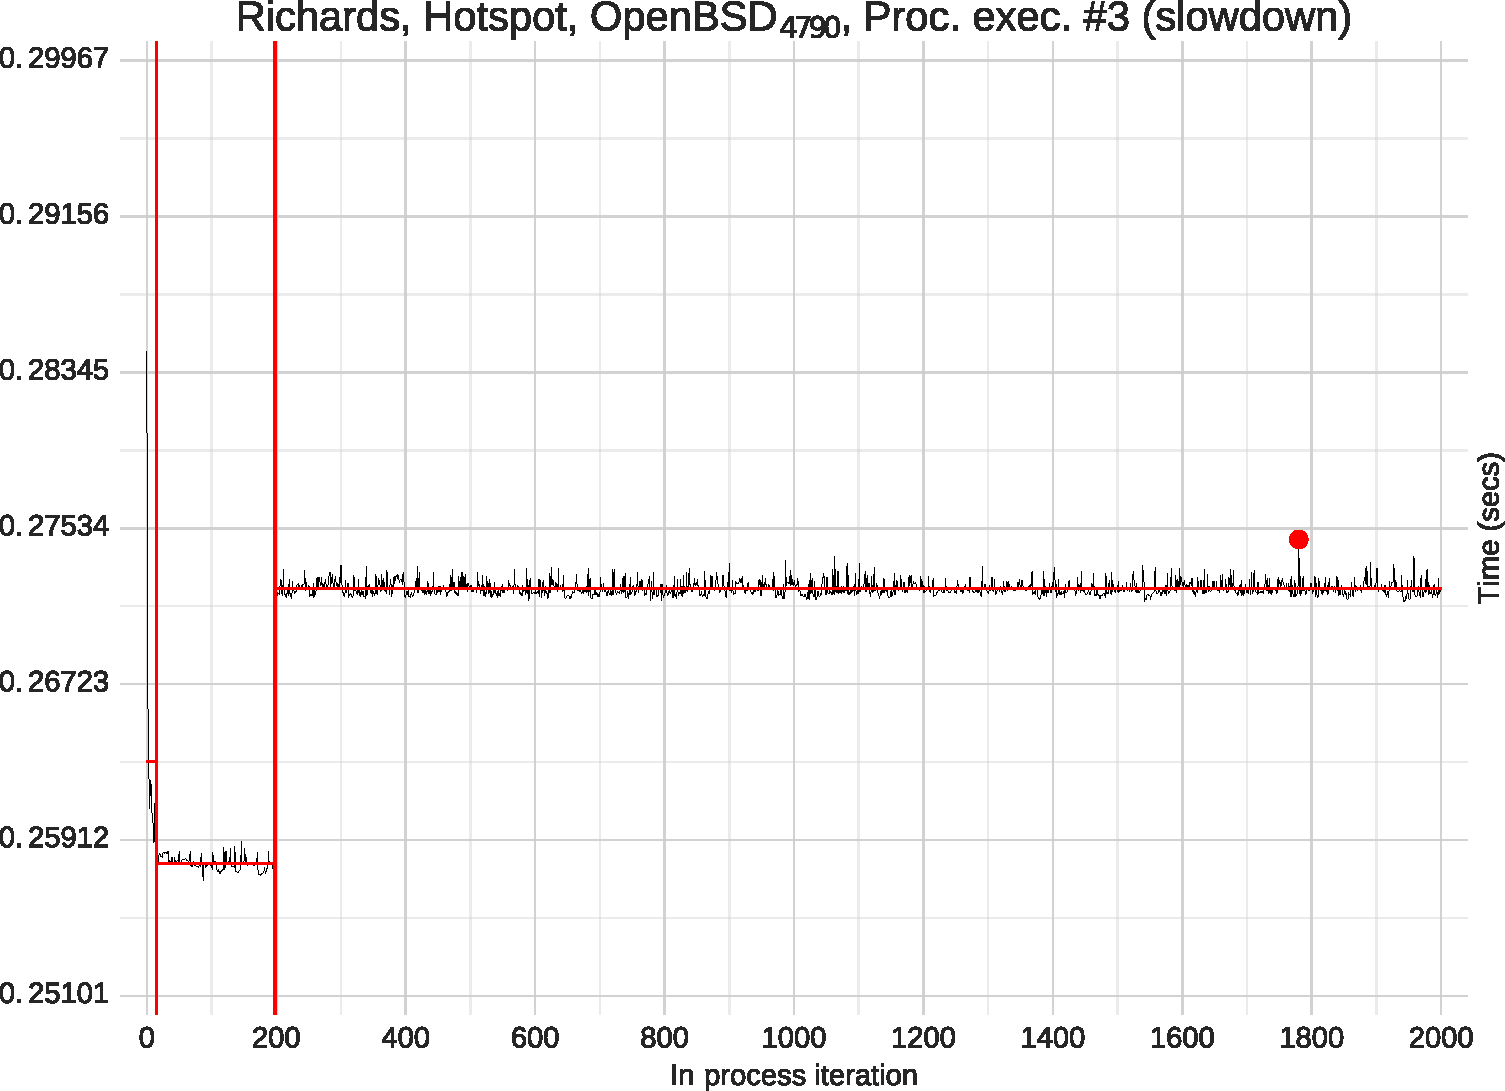
\includegraphics[width=.45\textwidth]{examples/changepoint_example.pdf}
\caption{An example of changepoint analysis on a run-sequence plot (a process
execution of Richards on HotSpot from \benchersix). This shows two changepoints
(the vertical red lines): one soon after startup; and another around iteration
200. The horizontal red lines are the means of the changepoint segments. The red
blob denotes a solitary outlier, which was discounted by the changepoint analysis.}
\label{fig:changepoint}
\end{figure}

In order to automate this, we use the \texttt{cpt.meanvar} function in the R
\texttt{changepoint} package~\cite{killick14changepoint}, passing $15\log{n}$ (where
$n$ is the time series length minus the number of outliers) to the
\texttt{penalty} argument. This function uses the PELT
algorithm~\citep{killick12optimal}, which can detect arbitrary numbers of changepoints; it
returns changepoint locations and the mean and variance
of each segment.



\subsection{Classifications}

\begin{figure}[t]
\begin{lstlisting}[label=lst:classification, xleftmargin=0cm, caption={The
classification algorithm for an individual process execution.}]
BOUND_PROPORTION = 0.001 # Proportion (i.e. 0.1%) of final segment to be used as a bound
ABSOLUTE_DELTA   = 0.001 # Time in seconds to be used as a bound
STEADY_STATE_LEN = 500   # Number of in-process iterations from the end for a steady state

# Given an ordered list of Segments -- each of which has "mean" and "end" attributes, the latter its absolute
# ending position in the sequence of in-process iterations -- return a string classifying the run sequence.
def classify(seq):
  lower_bound = min(seq[len(seq) - 1].mean * (1 - BOUND_PROPORTION), seq[len(seq) - 1].mean - ABSOLUTE_DELTA)
  upper_bound = max(seq[len(seq) - 1].mean * (1 + BOUND_PROPORTION), seq[len(seq) - 1].mean + ABSOLUTE_DELTA)
  cls = "flat"
  i = len(seq) - 2
  while i > -1:
    cur_seg = seq[i]
    i -= 1
    if cur_seg.mean >= lower_bound and cur_seg.mean <= upper_bound:
      continue
    elif cur_seg.end > len(seq) - STEADY_STATE_LEN:
      cls = "no steady state"
      break
    elif cur_seg.mean < lower_bound:
      cls = "slowdown"
      break
    assert(cur_seg.mean > upper_bound)
    cls = "warmup"
  return cls
\end{lstlisting}
\vspace{-.75cm}
\end{figure}

\edd{isn't this an infinite loop if any segment we try is in bounds? i is only decremented in the warmup case. Let's use a for loop?}
\laurie{python's for loop 'range' thing isn't well understood, so i'd prefer not to use it. you're right that i made an infinite loop though -- }

\sarah{The argument is a run sequence, but not really run-sequence plot, I would call the variable 'seq' rather than 'rsp'.}
\sarah{If this is pseudocode you might as well use 'class' for the string variable.}\laurie{i'd like it still to be executable in python}

Building atop changepoint analysis, we can then define useful classifications
for time-series data from VM benchmarks.

Before we can do so, we must
acknowledge the constraints that changepoint analysis works under: it has
no way of knowing what constitutes the `noise floor' in our problem domain; nor can it
guarantee to find identical means for very similar segments separated from
one another by a segment with a clearly distinct mean.
To understand the `noise floor' issue, it
is helpful to take an extreme example. Consider a long sequence of in-process
iterations all timed at 0.1001 seconds, followed by another long sequence timed
at 0.1002 seconds. A changepoint will be detected in the transition between the
two sequences, resulting in two changepoint segments. However, we know that in practice such a tiny absolute timing
delta is as likely to be the result of non-determinism inherent in a real
machine or OS as it is to be due to a benchmark or VM, and that it would be
better to consider them as being equal. It is tempting to merge such segments
together, but this fails to deal with separated segments. Consider a
benchmark which, after changepoint analysis has three segments: the first with a
mean of 1.0001 seconds, the second 0.2 seconds (perhaps whilst a JIT compiler is
in action), the third 1.0002 seconds. From our perspective, the first and final
segments are best considered as being equivalent, even though they are separated by a
segment which is clearly different. We therefore allow a small tolerance
when comparing a segment $s_i$ against the final segment $s_f$: if $s_i$'s
mean is within 0.1\% or 0.001s (whichever is greater) of $s_j$'s mean,
we consider the two equivalent. The reason for these two types of tolerance
is as follows. In short running benchmarks, a small number of external events can add an absolute
level of noise: in our experience readings often vary by a
little under 0.001s. In long running benchmarks, any individual external
event adds a relatively small relative amount of noise, but the cumulative
effect of many external events can add up, which we account for by allowing
a proportion of the running time.

With that in mind, we can define a simple classification algorithm for a process
execution, based on the special nature of the final changepoint segment. Since all our benchmarks run
for 2000 in-process iterations we (somewhat arbitrarily) define that a process
execution reaches a steady-state if all segments which cover the last 500
in-process iterations are considered equivalent to the final segment. If
not, we classify the process execution as \emph{no steady state} (\nosteadystate).
If a steady state is reached, we are then interested as to whether: all
segments are considered equivalent, leading to a classification of \emph{flat} (\flatc);
at least one segment is faster than the final segment leading to a classification
of \emph{slowdown} (\slowdown). If a steady state benchmark is not flat or a
slowdown, then by definition the final segment must be faster than
at least one preceding segment, leading to a classification of \emph{warmup} (\warmup).
Figure~\ref{lst:classification} shows an implementation of this algorithm.
We consider benchmarks whose behaviour is either flat or warmup
as `good' (flat benchmarks may be unobservably fast warmup), while
benchmarks which are either slowdown or no steady state are `bad'.

Based on this, we can then classify a (VM, benchmark)
\edd{Let's use tuple syntax, as it's hard to differentiate tuples from
bracketted prose. E.g. $\langle$VM, benchmark$\rangle$}\laurie{be my guest -- but note you'll need
to update the entire paper!} pair as follows:
if its process executions all share the same classification (e.g.~warmup) then
we classify the pair the same way (in this example, warmup); otherwise we classify the pair as
\emph{inconsistent}. There are then two sub-categories of inconsistent
benchmarks: `good' inconsistency (\goodinconsistent) is where all a (VM, benchmark) pair's process
executions are either flat or warmup; `bad' inconsistency (\badinconsistent) is
when one more process executions are no steady state or slowdown. Good inconsistency
occurs because some benchmarks are on the edge of our ability to detect warmup
vs.~flat execution; even minor measurement variation can cause a change between
these two good classifications. Bad inconsistency is always more troubling: it
means that, at least sometimes, users will experience poor performance.

\subsection{Timings}

For benchmarks which reach a steady state (i.e.~are \flatc, \warmup, or
\slowdown; or are inconsistent but only contain \flatc, \warmup, or \slowdown)
we report the number of iterations and the time in seconds to reach the steady state,
as well as the performance of the steady state itself in seconds (defined as
the final changepoint segment's mean). For the latter two measures, we report the median time
over all 10 process executions, and report 99\% confidence intervals (bootstrapped
with 10000 iterations, sampling with replacement).


\section{Results}
\label{sec:results}

\begin{table}
\begin{center}
\begin{tabular}{lccc}
\toprule
Class.         & \bencherthree & \bencherfive & \benchersix \\
\midrule
               & \multicolumn{3}{c}{(VM, benchmark) pairs} \\
\flatc         & \bencherthreevmbenchpairsflatpercentage\% & \bencherfivevmbenchpairsflatpercentage\% & \benchersixvmbenchpairsflatpercentage\% \\
\warmup        & \bencherthreevmbenchpairswarmuppercentage\% & \bencherfivevmbenchpairswarmuppercentage\% & \benchersixvmbenchpairswarmuppercentage\% \\
\slowdown      & \bencherthreevmbenchpairsslowdownpercentage\% & \bencherfivevmbenchpairsslowdownpercentage\% & \benchersixvmbenchpairsslowdownpercentage\% \\
\nosteadystate & \bencherthreevmbenchpairsnosteadystatepercentage\% & \bencherfivevmbenchpairsnosteadystatepercentage\% & \benchersixvmbenchpairsnosteadystatepercentage\% \\
\inconsistent  & \bencherthreevmbenchpairsinconsistentpercentage\% & \bencherfivevmbenchpairsinconsistentpercentage\% & \benchersixvmbenchpairsinconsistentpercentage\% \\
\midrule
               & \multicolumn{3}{c}{Process executions} \\
\flatc         & \bencherthreeflatpercentage\%          & \bencherfiveflatpercentage\%          & \benchersixflatpercentage\% \\
\warmup        & \bencherthreewarmuppercentage\%        & \bencherfivewarmuppercentage\%        & \benchersixwarmuppercentage\% \\
\slowdown      & \bencherthreeslowdownpercentage\%      & \bencherfiveslowdownpercentage\%      & \benchersixslowdownpercentage\% \\
\nosteadystate & \bencherthreenosteadystatepercentage\% & \bencherfivenosteadystatepercentage\% & \benchersixnosteadystatepercentage\% \\
\bottomrule
\end{tabular}
\end{center}
\caption{Relative proportions of classifiers across benchmarking machines.
Classifiers key: \flatc: flat, \warmup: warmup, \slowdown: slowdown,
\nosteadystate: no steady state, \inconsistent: inconsistent.}
\label{tab:summarystats}
\end{table}

\begin{table*}[t]
\centering
\input{bencher3.table}
\caption{Benchmark results for \bencherthree. For processes which reach a steady
state: \emph{steady iter (\#)} is the median in-process iteration that the steady
state was reached at; \emph{steady iter (s)} is the wall-clock time since the
beginning of the process execution that the steady state was reached;
\emph{steady perf (s)} is the median performance of the steady state segment
across all process executions. We give the
constituent classifications of inconsistent benchmarks e.g.~\inconsistent(2\slowdown, 8\warmup) means
2 of the process executions were slowdown, and 8 warmup.}
\label{tab:mainresults}
\end{table*}

% Excluding the empty benchmark we have:
%  Linux: 6 benchmarks, 8 VMs == 48 benchmarks *but* we skip 2
%        (fasta/JRubyTruffle and Richards/HHVM), so actually 46
%  OpenBSD: 6 benchmark, 5 VMs = 30 benchmarks
%  So 2*Linux + 1*OpenBSD = 2 * 46 + 1 * 30 = 122 benchmarks
%  Num process execs: 122 * 10 = 1220
%  Num in-process iters: 1220 * 2000 = 2,440,000

Our experiment consists of \totalpexecs{} process executions and \totaliterations{} in-process
iterations. Table~\ref{tab:summarystats} summarises the (VM, benchmark) pairs
and process executions for each benchmarking machine. Taking \bencherthree
as a representative example,
\FPeval{\result}{round(\bencherthreevmbenchpairsflatpercentage+\bencherthreevmbenchpairswarmuppercentage,1)}%
\result\% of (VM, benchmark) pairs and
\FPeval{\result}{round(\bencherthreeflatpercentage+\bencherthreewarmuppercentage,1)}%
\result\% of process executions have `good' warmup (\flatc, \warmup) (for comparison, \bencherfive
is
\FPeval{\result}{round(\bencherfivevmbenchpairsflatpercentage+\bencherfivevmbenchpairswarmuppercentage,1)}%
\result\% and
\FPeval{\result}{round(\bencherfiveflatpercentage+\bencherfivewarmuppercentage,1)}%
\result\% respectively and \benchersix is
\FPeval{\result}{round(\benchersixvmbenchpairsflatpercentage+\benchersixvmbenchpairswarmuppercentage,1)}%
\result\% and
\FPeval{\result}{round(\benchersixflatpercentage+\benchersixwarmuppercentage,1)}%
\result\% respectively, though the latter runs fewer benchmarks). Fewer (VM, benchmark) pairs than process executions have `good'
warmup because some inconsistent (VM, benchmark) pairs have some `good' warmup
process executions. On \bencherthree
\bencherthreevmbenchpairsslowdownpercentage\% of (VM, benchmark) pairs slowdown
and \bencherthreevmbenchpairsinconsistentpercentage\% are inconsistent
(with over two thirds of those being obviously `bad'); \bencherfive and
\benchersix are broadly similar. Taking \bencherthree as an example,
one third of its (VM, benchmark) pairs are `bad', clearly invalidating
Hypothesis H1.

Table~\ref{tab:summarystats} clearly shows that the results from \bencherthree
and \bencherfive (both running Linux but on moderately different hardware) are
comparable, with the relative proportions of all measures being only a few
percent different. \benchersix (running OpenBSD, but on the same hardware as
\bencherthree) is somewhat different. This is in large part because it
is unable to run benchmarks on Graal, HHVM, and JRuby+Truffle (see
Section~\ref{openbsd porting}): of the benchmarks it can run, most behave
similarly, with the notable exception of LuaJIT, whose benchmarks are more often
classified as non-flat (see Table~\ref{tab:bencher6results} in the Appendix).
With that in mind, we believe that our results are a fairly clear validation of
Hypothesis H2.

Looking at one machine's data brings out further detail. For
example, Table~\ref{tab:mainresults} (with data from \bencherthree)
enables to make us several observations. Of the 6 benchmarks, only \nbody comes
close to `good' warmup behaviour on all
VMs on all machines (the one C slowdown excepted): the other 5 benchmarks all have at least one VM which consistently
slows down. Second, there appears to be a bimodal pattern for the number
of in-process iterations required to reach a steady state (when it exists): VMs
tend either to reach it very quickly (often in 10 or fewer in-process iterations)
or take hundreds of in-process iterations. Those that take a long time
to stabilise are troubling, because previous benchmarking methodologies
will not have run them long enough to see this steady state emerge.
Finally, there seems to be very little
correlation between the time it takes a VM to reach a steady state and the
performance of that steady state: i.e.~it does not seem to be the case that VMs
which take a long time to warmup are creating more efficient
steady-state code.


\subsection{Warmup Plots}

To understand why we see so many unexpected cases, we created a series of plots
for process executions. All
plots have in-process iteration number on the $x$-axis. For $y$-axes:
\emph{run-sequence plots} show wall-clock time; and (on Linux) \emph{core-cycle plots} show
the processor cycle count per-core.
The run-sequence and core-cycle plots in Figures~\ref{fig:examples:trad}, \ref{fig:examples:slowdown1},
and \ref{fig:examples:nosteadystate} show examples of traditional warmup, slowdown,
and no steady state respectively. Figure~\ref{fig:examples:inconsistent} shows
an example of inconsistent process executions.

\begin{figure}[t]
\centering
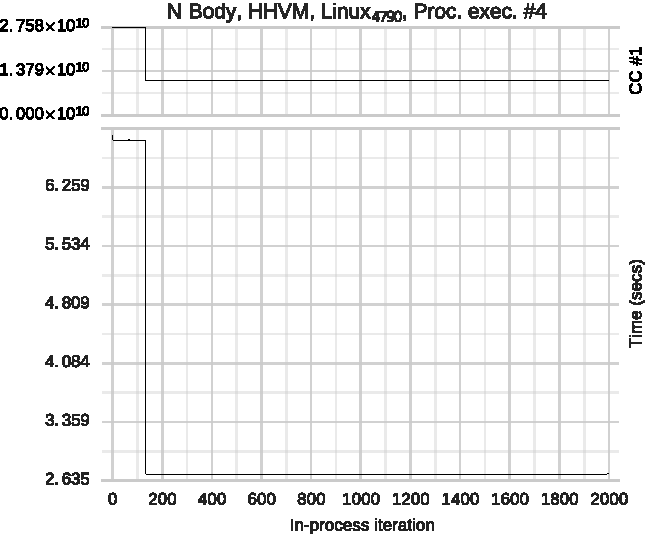
\includegraphics[width=.45\textwidth]{examples/new_warmup_no_migrate.pdf}
\caption{An example of traditional warmup behaviour with the n-body benchmark on
HHVM (process execution 4 of 10 run on \bencherthree). The run-sequence plot
(bottom) shows that warmup completed by in-process iteration \#134. The
core-cycle plot (top) shows that the main benchmark computation
occurred almost entirely on core 1: cores 0, 2 and 3 Cycle Counts (CC)
were low enough for us to classify them as `inactive', and we have thus elided them.}
\label{fig:examples:trad}
\vspace{-.2cm}
\end{figure}

\begin{figure}[t]
\centering
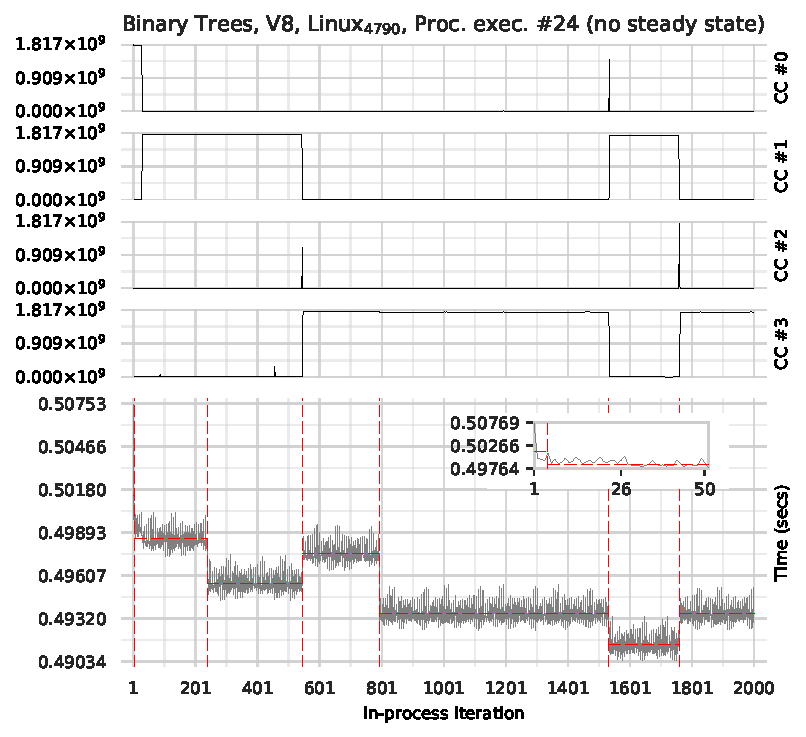
\includegraphics[width=.45\textwidth]{examples/new_no_steady.pdf}
\caption{No steady state. There is a small behavioural shift around iteration
950, where the VM migrates from (tickless) core 1 to (ticked) core 0.}
\label{fig:examples:nosteadystate}
\end{figure}

\begin{figure*}[t!]
\centering
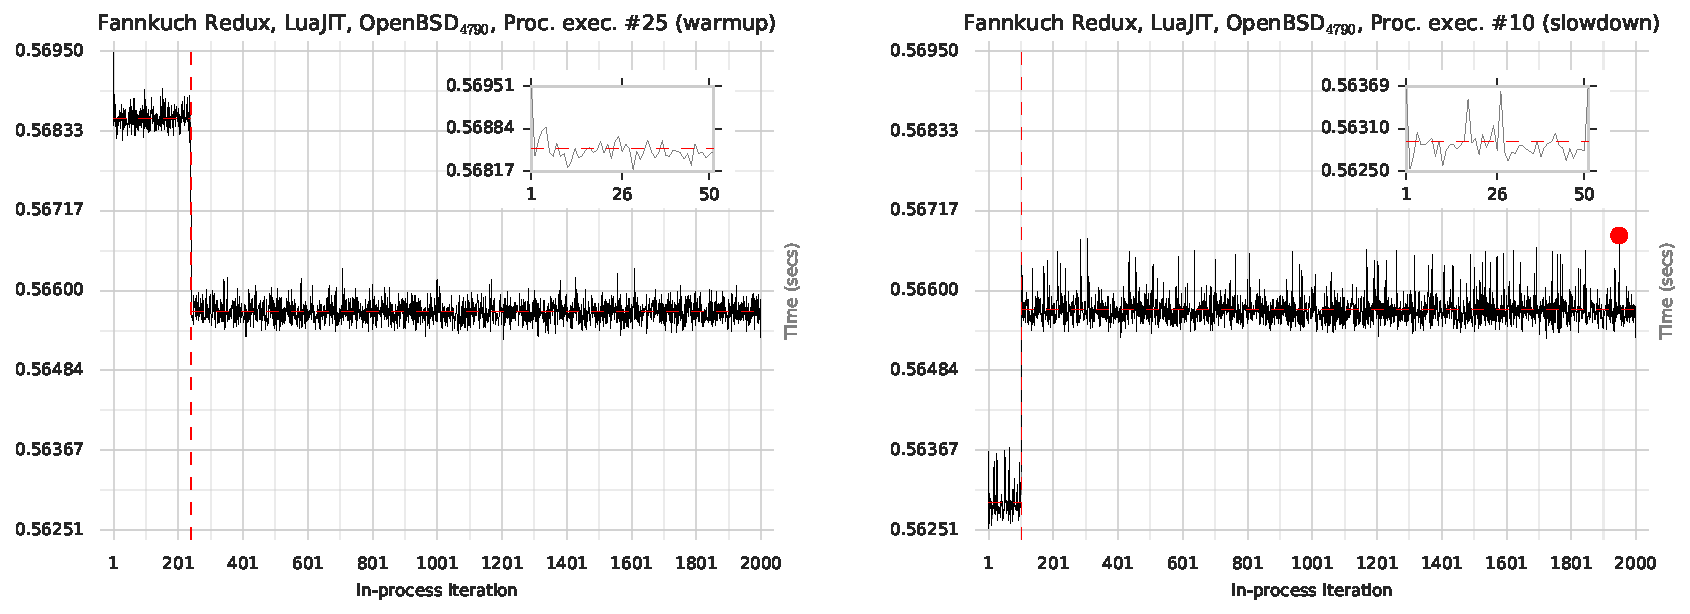
\includegraphics[width=.8\textwidth]{examples/new_inconsistent.pdf}
\caption{An example of inconsistent process executions for the same (machine, VM, benchmark) triple.}
\label{fig:examples:inconsistent}
\vspace{-.4cm}
\end{figure*}

\begin{figure}[!tbp]
\centering
\begin{minipage}[b]{0.45\textwidth}
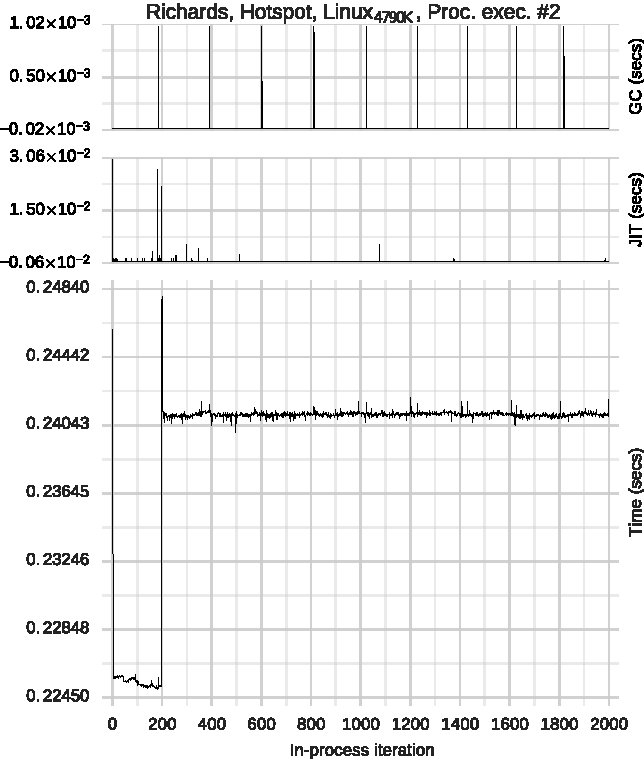
\includegraphics[width=\textwidth]{examples/new_miscomp.pdf}
\caption{Slowdown at in-process iteration \#199, with GC and JIT measurements
turned on. Although these additional measures add overhead, in this
case they make no observable difference to the main run-sequence graph. They
allow us to observe that the slowdown is correlated with two immediately preceding JIT compilation events
that may explain the drop in performance. Note that the
regular GC spikes have only a small effect on the time of in-process
iterations.}
\label{fig:examples:slowdown1}
\end{minipage}
\hfill
\begin{minipage}[b]{0.45\textwidth}
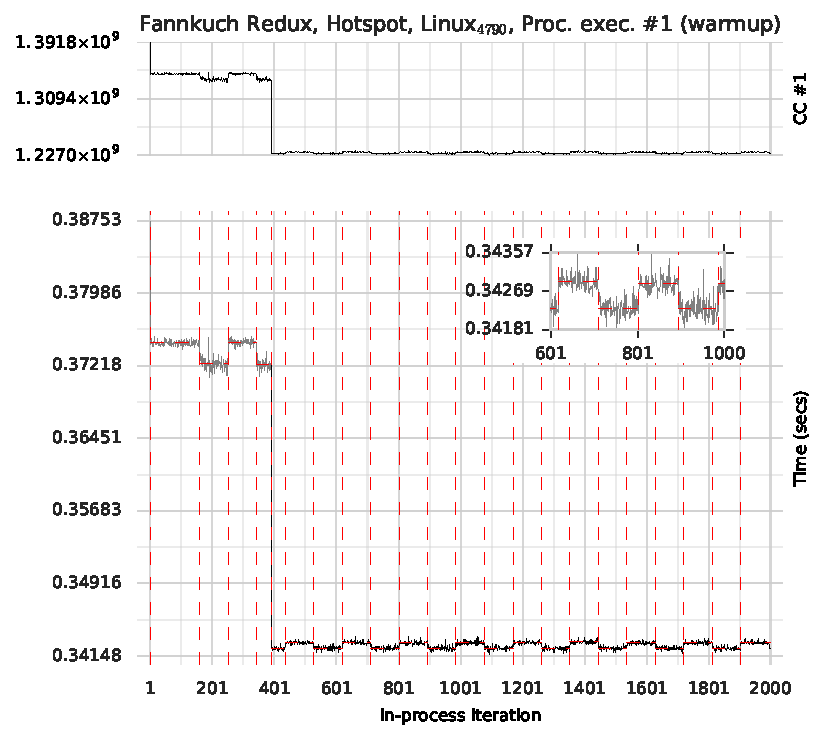
\includegraphics[width=\textwidth]{examples/new_cyclic.pdf}
\caption{Cycles in wall-clock times and core-cycle counts.}
\label{fig:examples:cycles}
\end{minipage}
\end{figure}

Core-cycle plots help us understand how VMs use, and how the OS schedules,
threads. Benchmarks running on single-threaded VMs are characterised by a high
cycle-count on one core, and very low (though never quite zero) values on all
other cores. Such VMs may still be migrated between cores during a process
execution, as can be clearly seen in Figure~\ref{fig:examples:nosteadystate}.
Although multi-threaded VMs can run JIT compilation and / or GC in parallel,
it is typically hard to visually detect such parallelism as it tends to be
accompanied by frequent migration between cores.
However, it can often easily be seen that several cores are active during the first few
in-process iterations whilst JIT compilation occurs.


\subsection{Cyclic data}

We suspected that enough benchmarks
would exhibit cyclic behaviour (as seen in Figure~\ref{fig:examples:cycles}) to
require special support in our automated analysis. To quantify this, we took one process
execution from each benchmark run on \bencherthree, removed the first 1500
in-process iterations, and generated an autocorrelation plot for the remainder
(in similar fashion to \kalibera). 4 (VM, benchmark) pairs showed what we have come to
call `fully cyclic' behaviour, where all in-process iterations repeat in a
predictable pattern; 8 showed `partially cyclic' behaviour, where
most iterations are noise around a mean, but every $n$ iterations there is a
predictable and significant peak (with $n$ varying from 5 to 19).

For partially cyclic data, or fully cyclic data with a large period (as in
Figure~\ref{fig:examples:cycles}), our automated analysis handles the situation
appropriately (classifying Figure~\ref{fig:examples:cycles} as no steady state).
However, changepoint analysis cannot currently identify small cycle periods in
fully cyclic data. Since this only happens for 2
of 47 (VM, benchmark) pairs, both of which have a small absolute difference between the
cycle's elements, we consider this a minor worry.


\subsection{The Effects of Compilation and GC}
\label{sec:deepdive}

The large number of non-warmup cases in our data led us to make the following hypothesis:
\begin{description}
  \item[H3] Non-warmup process executions are largely due to JIT compilation or GC events.
\end{description}
To test this hypothesis, we made use of the fact that both HotSpot and PyPy allow
information about the duration of JIT compilation and GC to be recorded. Since
recording this additional data could potentially change the results we collect,
it is only collected when \krun is explicitly set to `instrumentation mode'. An
example instrumentation-plot can be seen in the slowdown of
Figure~\ref{fig:examples:slowdown1} where there is a clear correlation (though we
cannot be entirely sure that it is a causation) between a JIT compilation and
the slowdown. However, some other notably odd examples have no such correlation,
as can be seen in Figure~\ref{fig:goodcomp}.

The relatively few results we have with GC and JIT compilation events, and the lack of a clear
message from them, means that we feel unable to validate or invalidate
Hypothesis H3. Whilst some non-warmups are plausibly explained by GC or JIT compilation events, many are not, at
least on HotSpot and PyPy. When there is no clear explanation, we have very little idea what might be
the cause of the unexpected behaviour. It may be that obtaining similar data
from other VMs may help clarify this issue, but not all VMs support this
feature and, in our experience, those that do support it do not always
document it accurately.

\begin{figure}[tbp]
\centering
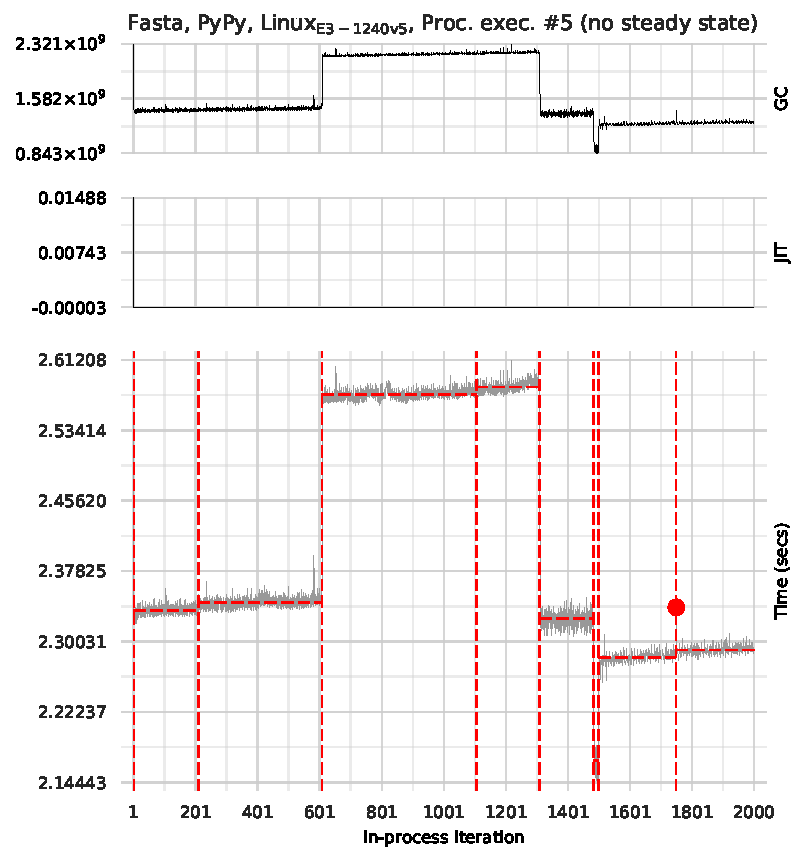
\includegraphics[width=.45\textwidth]{examples/new_good_comp.pdf}
\caption{The cyclic example from Figure~\ref{fig:examples:cycles} with
GC and JIT compilation instrumentation enabled. The additional overhead
changes some of the details in the first half of the process
execution, but the second half is unchanged. As this example shows, the
cycles are not correlated with GC (of which there is none) or JIT compilation.}
\label{fig:goodcomp}
\end{figure}

\section{Startup Time}
\label{sec:startup}

The data presented thus far in the paper has all been collected after the VM has
started executing the user program. The period between a VM being
invoked and it executing the first line of the user program is the VM's \emph{startup} time,
and is an important part of a VM's real-world performance.

A small modification to \krun enables us to measure startup. We prepend each VM
execution command with a small C wrapper, which prints out wall-clock time
before immediately executing the VM itself; and, for each language under
investigation, we provide a `dummy' iterations runner which simply prints out
wall-clock time. In other words, we measure the time just before the VM is loaded
and at the first point that a user-level program can execute code on the VM; the
delta between the two is the startup time. For each VM we run 200 process
executions (for startup, in-process executions are irrelevant,
as the user-level program completes as soon as it has printed out wall-clock
time).

Table~\ref{fig:startup} shows startup times from both \bencherthree and \benchersix. Since
\krun reboots before each process execution, these are measures of a `cold'
start and thus partly reflect disk speed etc. (though both machines load VMs
from an SSD). As this data clearly shows, startup time varies significantly amongst VMs:
taking C as a baseline, the fastest VM (LuaJIT) is around 2x slower, whilst the
slowest VM (JRuby+Truffle) is around 1000x slower, to startup.

\begin{table}[t]
\centering
\input{startup.table}
\caption{VM startup time (in seconds with 99\% confidence intervals).}
\label{fig:startup}
\end{table}


\section{Threats to Validity}
\label{sec:threats}

While we have designed our experiment as carefully as possible, we do not
pretend to have controlled every possibly confounding variable. It
is inevitable that there are further confounding variables that
we are not aware of, which may have coloured our results.

We have tried to gain a partial understanding of the effects of different
hardware on benchmarks by using machines with the same OS but
different hardware. However, while the hardware between the two is
different, more distinct hardware (e.g.~a non-x86 architecture)
is more likely to uncover hardware-related differences.
However, hardware cannot be varied in isolation from software:
the greater the differences in hardware, the more likely that JIT compilers
compilers are to use different components (e.g.~different code generators).
Put another way, an apples-to-apples comparison across very different
hardware is often impossible, because the `same' software is itself different.

We have not systematically tested whether rebuilding VMs effects warmup, an
effect noted by \kalibera, though which seems to have little effect on
the performance of JIT compiled code~\cite{barrett15approaches}. However, since measuring warm-up largely
involves measuring code that was not created by a JIT compiler, it is possible
that these effects may impact upon our experiment. To a limited extent, the
rebuilding of VMs that occurred on each of our benchmarking machines gives
some small evidence as to this effect, or lack thereof.

The checksums we added to benchmarks ensure that, at a user-visible level, each
performs equivalent work in each language variant. However, it is impossible to
say whether each performs equivalent work at the lowest level or not. For
example, choosing to use a different data type in a language's core library may
substantially impact performance. There is also the perennial problem as to the
degree to which an implementation of a benchmark should respect other
language's implementations or be idiomatic (the latter being likely to
run faster). From our perspective, this possibility is somewhat less important,
since we are interested in the warmup patterns of reasonable programs,
whether they be the fastest possible or not. It is however possible that by
inserting checksums we have created unrepresentative benchmarks, though
this complaint could arguably be directed at the unmodified benchmarks too.

Although we have minimised the number of system calls that our in-process
iterations runners make, we cannot escape them entirely. For example,
on both Linux and OpenBSD \texttt{clock\_gettime()} (which we use to obtain
monotonic wall-clock time) contains what is effectively a spin-lock,
meaning that there is no guarantee that it returns within a fixed bound.
%\footnote{See \texttt{binuptime} in \texttt{sys/kern/kern\_tc.c} in the
%OpenBSD source code and \texttt{getrawmonotonic} in
%\texttt{kernel/time/timekeeping.c} in the Linux source code.}
Fortunately, in practise, \texttt{clock\_gettime} returns far quicker than the granularity
of any of our benchmarks. \label{aperf/mperf error} The situation
on Linux is complicated by our reading of core cycle, APERF, and MPERF
counters via MSR device nodes: we call \texttt{lseek} and \texttt{read}
between each in-process iteration (we keep the files open across all
in-process iterations to reduce the open/close overhead).
These calls are more involved than \texttt{clock\_gettime}:
as well as the file system overhead, reading from a MSR device
node triggers inter-processor interrupts to schedule an \texttt{RDMSR}
instruction on the desired core (causing the running core to save its registers etc.).
We are not currently aware of a practical way to lower these costs.

Although \krun does as much to control CPU clock speed as possible, modern CPUs
do not always respect operating system requests. On Linux, we use the
APERF/MPERF ratio to check for frequency changes. Although the hoped-for
ratio is precisely 1, there is often noticeable variation around this value due to the
cost of reading these counters. On cores
performing active computation, the error is small (around 1\% in our
experience), but on inactive cores it can be relatively high (10\% or more is
not uncommon; in artificially extreme cases, we have observed up to 200\%).
In order to verify that there were no frequency changes during benchmarking,
we wrote a simple checking tool. For each in-process iteration, it first checks
the corresponding cycle-count data: since active cores generally have
cycle-counts in the billions, we conservatively classify inactive
cores as those with cycle-counts in the low millions. Active cores are then
checked for an APERF/MPERF ratio between $1 \pm 0.015$. All active cores in our
experiment were within these limits, strongly suggesting that our experiment
experienced no unexpected CPU frequency changes.

Our experiments allow the kernel to run on the same core as benchmarking code.
We experimented extensively with CPU pinning, but eventually abandoned it. After
being confused by the behaviour of Linux's \texttt{isolcpus} mechanism (whose
semantics changes between a normal and a real-time kernel), we used CPU shielding
(\texttt{cset shield}) to pin the benchmarks to the 3 non-boot cores on our
machines. However, we then observed notably worse performance for VMs such as
HotSpot. We suspect this is because such VMs query the OS for the number of
available cores and create a matching number of compilation threads; by reducing
the number of available cores, we accidentally forced two of these threads to
compete for a single core's resources.

In controlling confounding variables, our benchmarking environment necessarily
deviates from standard configurations. It is possible that in so doing, we have
created a system that shows warmup effects that few people will ever see in
practise. However, our judgement is that this is preferable to running on a
system that is likely to introduce substantial noise into our readings.


\section{Related work}

There are two works we are aware of which explicitly note unusual warmup
patterns. Whilst running benchmarks on HotSpot, Gil et
al.~\cite{gil11microbenchmark} observed inconsistent process executions
(e.g.~recursiveErgodic), and benchmarks that we could classify as no
steady state (listBubbleSort) and slowdown (arrayBubbleSort). By running a
greater number of (somewhat larger) benchmarks on a number of VMs, and executing
them in a more tightly controlled execution environment, our results can be seen
as significantly strengthening Gil et al.'s observations. Our work also adds an
automated approach to identifying when warmup has occurred.
\kalibera note the
existence of what we have called cyclic behaviour (in the context of benchmarking,
they then require the user to
manually pick one part of the cycle for measurement~\cite{kalibera13rigorous}):
the data from our experiment seems to be less often cyclic, though we have no
explanation for why.


\section{Conclusions}
\label{sec:conclusion}

Warmup has previously been an informally defined term~\cite{seaton15phd} and in this
paper we have shown cases where the definition fails to hold. Through a carefully
designed experiment, and an application of a new statistical method, we hope
to have helped give the study of warmup a firmer base.

Although we are fairly experienced in designing and implementing
experiments, the experiment in this paper took far more time than we expected
--- over 2 full person years. In part this is because there is limited precedent for such detailed
experiments. Investigating possible confounding variables, understanding how to
control them, and implementing the necessary checks, all took time. In many
cases, we had to implement small programs or systems to understand a variable's
effect (e.g.~that Linux allows a process to allocate memory beyond that
specified in the soft and hard \texttt{ulimit}). However, we are realistic that
few people will have the time or energy to institute all the controls that we
implemented. An open question is which of the controls are the most significant
in terms of producing a reliable experiment. The large number of partly
inter-locking combinations means that we estimate that untangling this will
require 3--6 months of experimental running time.

Our results suggest to us some tentative guidelines for VM
developers and users. First, simply running benchmarks for a larger number of
in-process iterations helps understanding of a VM's long-term
performance stability. Second, as a community, we need to accept that a steady
state of peak performance is not guaranteed to exist. Third, the significant
differences in warmup time between VMs strongly suggest that VM benchmarking
should always include warmup time. Fourth, we suspect that some of the odd
results we have seen result from over-training VM heuristics on small sets of
benchmarks. The machine-learning community's approach may apply
equally well to VMs: using a training set to devise heuristics, and then
benchmarking the resulting system(s) on a separate validation system. Fifth, we suspect
that a reliance on small suites of benchmarks means that only
small parts of VMs are being benchmarked effectively: we are increasingly of the
opinion that benchmarking quality and quantity are tightly related, and that VMs
need more benchmarks.

\begin{acks}
We are particularly grateful to Vincent Knight
who helped put together this paper's team. Chris Seaton
helped integrate JRuby+Truffle into our experiment. We also thank (in alphabetical order) Dave Dice, Kenny
Gross, Tim Harris, Dave Ungar, Mario Wolczko for comments and suggestions; any
errors and infelicities are our own. This research was funded by the EPSRC
Cooler (EP/K01790X/1) grant and Lecture (EP/L02344X/1) fellowship.
\textbf{Transparency:} Three of this paper's authors have contributed
to the PyPy project, and one is an OpenBSD developer. The
King's group has received several funding gifts from Oracle Labs.
\end{acks}


\bibliographystyle{ACM-Reference-Format}
%\citestyle{acmauthoryear}   %% For author/year citations
\bibliography{bib}

\clearpage

\appendix

\noindent In this appendix, we first show that our statistical method
can be applied to well known benchmarking suites (Appendix~\ref{sec:existing})
before showing the complete warmup data from our experiment
(Appendix~\ref{app:mainresults}). We
then present a curated selection of interesting run-sequence / core-cycle /
APERF/MPERF plots. The complete series of plots is available in a separate
document.


\section{Applying the Statistical Method to Existing Benchmark Suites}
\label{sec:existing}

The statistical method presented in Section~\ref{sec:stats} is not limited to data
produced from Krun. To demonstrate this, we have applied it to two standard
benchmark suites: DaCapo~\cite{dacapo06} (Java) and Octane~\cite{octane}
(JavaScript). We ran both for 10 process executions and 2000 in-process
iterations without reboots, temperature control etc.: DaCapo on \bencherthree;
and Octane on \bencherseven (a Xeon machine, with a software setup
similar to \bencherthree).\footnote{The large amount of CPU time our
experiments require meant that we ran out of time to run Octane on \bencherthree
before paper submission. For the final paper, we will run DaCapo and Octane on
the same machine. Although we do not expect this to result in significant
changes to the data, it will reduce a source of variation.}

We ran DaCapo (with its default benchmark size) on Graal and HotSpot. As it already has support for
altering the number of in-process executions, we used it without modification.
However, we were unable to run 4 of its 14 benchmarks: \texttt{batik}
crashes with a \texttt{Invocation\-Target\-Exception}; \texttt{eclipse},
\texttt{tomcat}, and (intermittently) \texttt{tradesoap} fail their own internal
validation checks.

We ran Octane on SpiderMonkey (\spidermonkeyversion, a JIT compiling VM for JavaScript) and V8.
We replaced its complex runner (which reported timings with a non-monotonic
microsecond timer) with a simpler alternative (using a monotonic millisecond
timer). We also had to decide on an acceptable notion of `iteration'. Many of Octane's
benchmarks consist of a relatively quick `inner benchmark'; an `outer benchmark'
specifies how many times the inner benchmark should be run in order to make an
adequately long running benchmark. We recorded 2000 iterations of the outer benchmark; our runner
fully resets the benchmark and the random number generator between each
iteration. The \texttt{box2d}, \texttt{gameboy}, \texttt{mandreel} benchmarks do
not properly reset their state between runs, leading to run-time errors we have
not been able to fix; \texttt{typescript}'s reset function, in contrast,
frees constant data needed by all iterations, which we were able
to easily fix. When run for 2000 iterations, \texttt{CodeLoadClosure},
\texttt{pdfjs}, and \texttt{zlib} all fail due to memory leaks. We were able to
easily fix \texttt{pdfjs} by emptying a global list after each iteration, but not the
others. We therefore include 12 of Octane's benchmarks (including lightly
modified versions of \texttt{pdfjs} and \texttt{typescript}).
Because we run fewer benchmarks, our modified runner is unable to fully
replicate the running order of Octane's original runner. Since Octane runs all
benchmarks in a single process execution, this could affect the performance of
later benchmarks in the suite.

Table~\ref{tab:dacapo} shows the full DaCapo results. Graal and HotSpot both
perform similarly. The luindex benchmark is consistently a slowdown on Graal,
and mostly a slowdown on HotSpot. Jython is notably inconsistent on both VMs. In
summary, even on this most carefully designed of benchmark suites, only 70\%
of (VM, benchmark) pairs have `good' warmup.

Table~\ref{tab:octane} shows the full Octane results. These are notably less
consistent than the DaCapo results, with SpiderMonkey being somewhat less
consistent than V8. In summary, only 45.8\% of (VM, benchmark) pairs have `good'
warmup.

As these results show, our automated statistical method produces satisfying
results even on existing benchmark suites that have not been subject to the
\krun treatment. Both DaCapo and (mostly) Octane use much larger benchmarks than
our main experiment. We have no realistic way of understanding to what extent
this makes `good' warmup more or less likely. For example, it is likely that
there is CFG non-determinism in many of these benchmarks; however, their larger
code-bases may give VMs the ability to `spread out' VM costs, making smaller
blips less likely.


\begin{table*}[t]
\centering
\input{dacapo.table}
\caption{DaCapo results.}
\label{tab:dacapo}
\end{table*}


\begin{table*}[t]
\centering
\input{octane.table}
\caption{Octane results.}
\label{tab:octane}
\end{table*}


\section{Further Results}
\label{app:mainresults}
\label{app:dacapo}
\label{app:octane}

\noindent The main experiment's results for \bencherfive and \benchersix can be
seen in Tables~\ref{tab:bencher5results} and \ref{tab:bencher6results}.

\begin{table*}[t]
\centering
\input{bencher5.table}
\captionof{table}{Benchmark results for \bencherfive.}
\label{tab:bencher5results}
\end{table*}

\begin{table*}[t]
\centering
\input{bencher6.table}
\caption{Benchmark results for \benchersix.}
\label{tab:bencher6results}
\end{table*}

\clearpage
\onecolumn

\section{Curated Plots}
\label{sec:curatedplots}

\noindent The remainder of this appendix shows curated plots: we have selected
4 interesting plots from each classification, to give readers a sense of
the range of data obtained from our experiment. A separate document contains the
complete series of plots.

\clearpage
\twocolumn

\subsection{Examples of Warmup Behaviour}
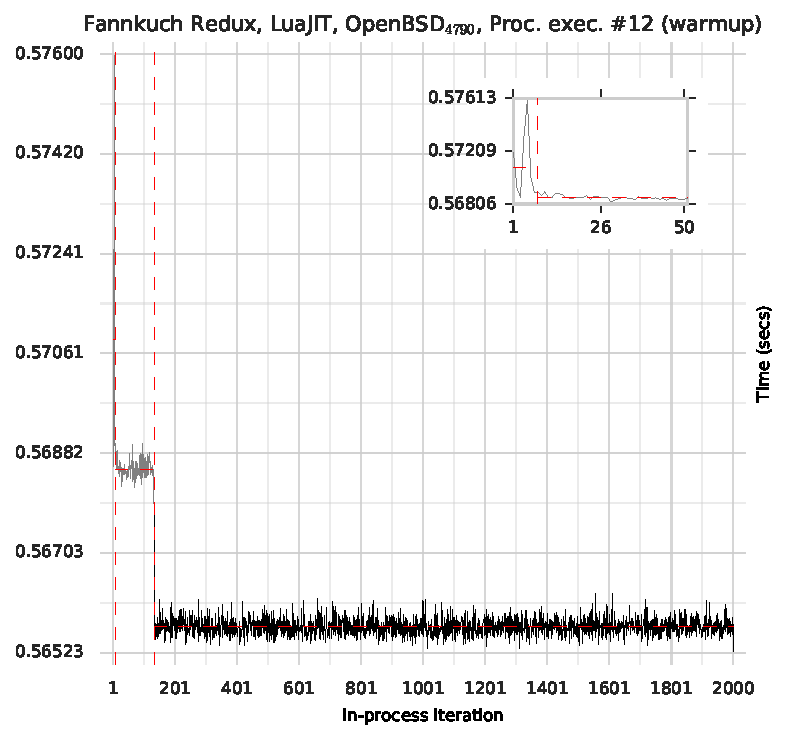
\includegraphics[width=.45\textwidth]{category_examples/warmup/warmup0.pdf}
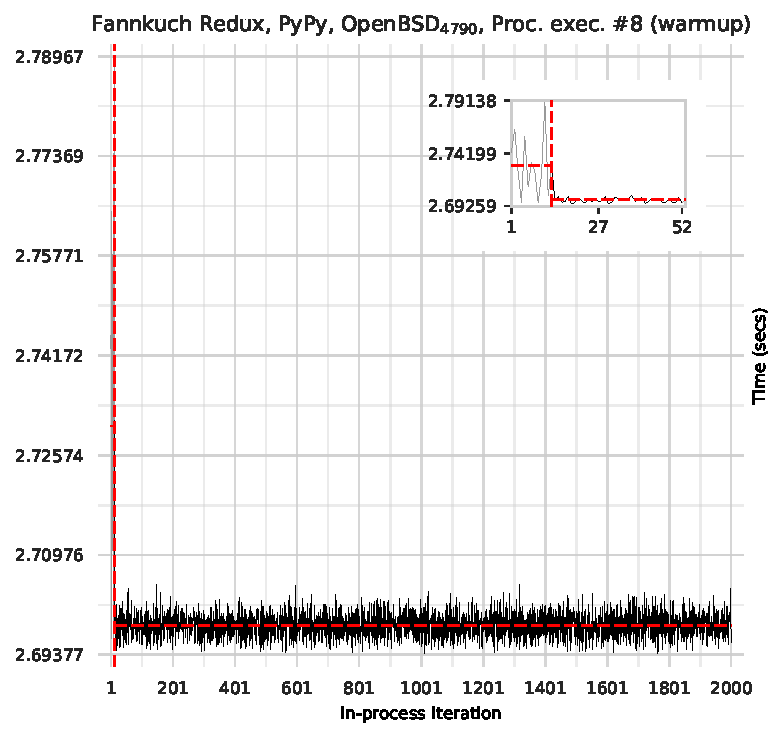
\includegraphics[width=.45\textwidth]{category_examples/warmup/warmup1.pdf}
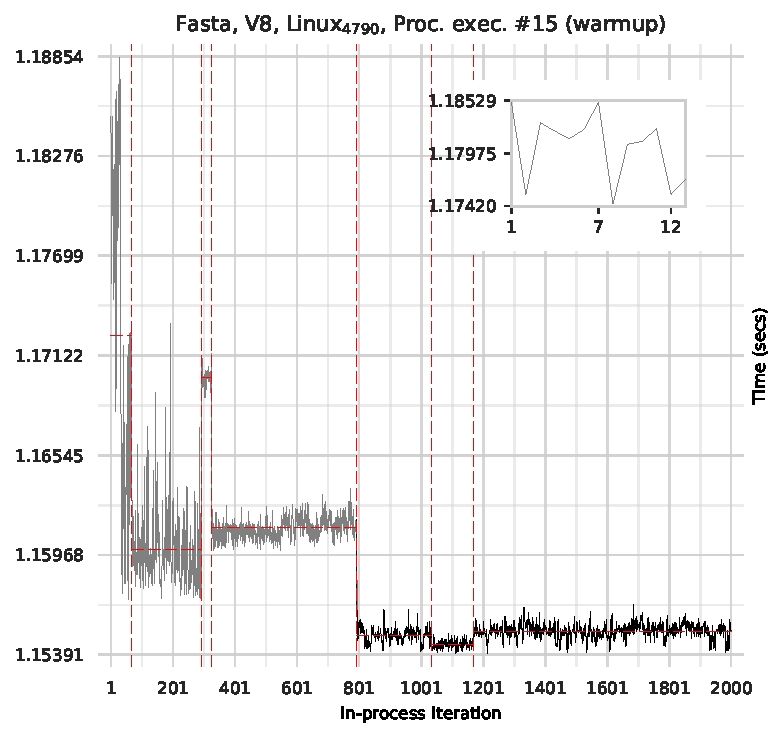
\includegraphics[width=.45\textwidth]{category_examples/warmup/warmup2.pdf}
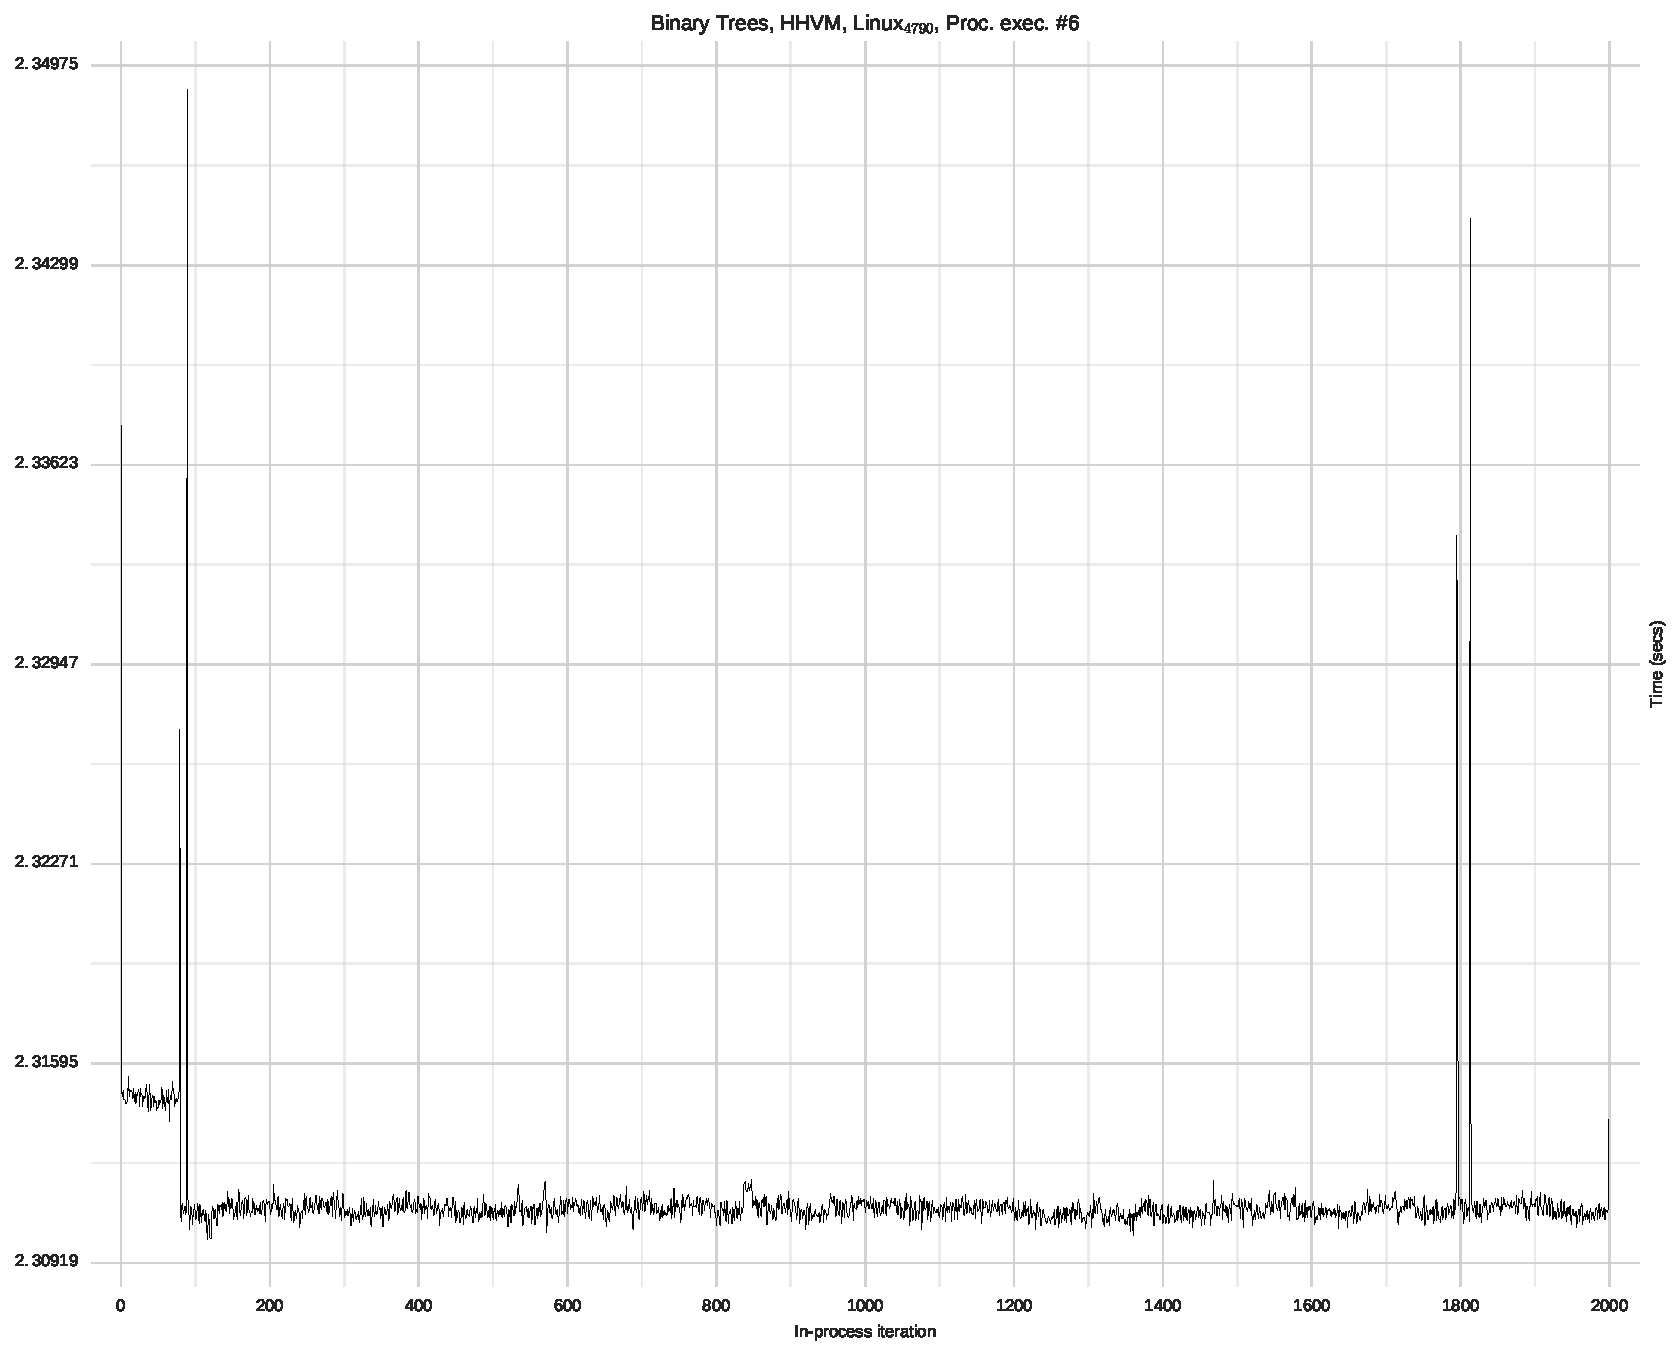
\includegraphics[width=.45\textwidth]{category_examples/warmup/warmup3.pdf}
% 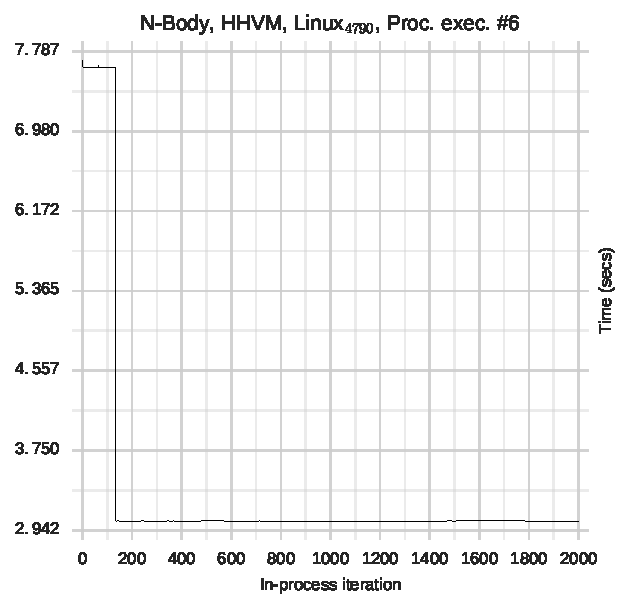
\includegraphics[width=.45\textwidth]{category_examples/warmup/warmup4.pdf}

\clearpage

\subsection{Examples of Flat Behaviour}
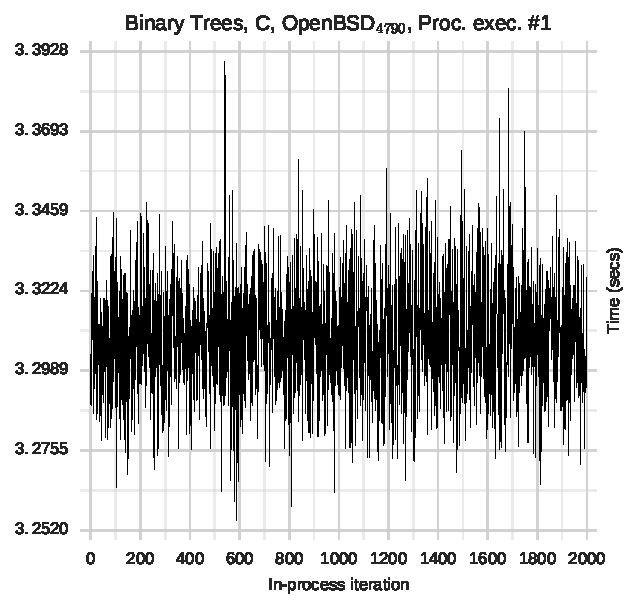
\includegraphics[width=.45\textwidth]{category_examples/flat/flat0.pdf}
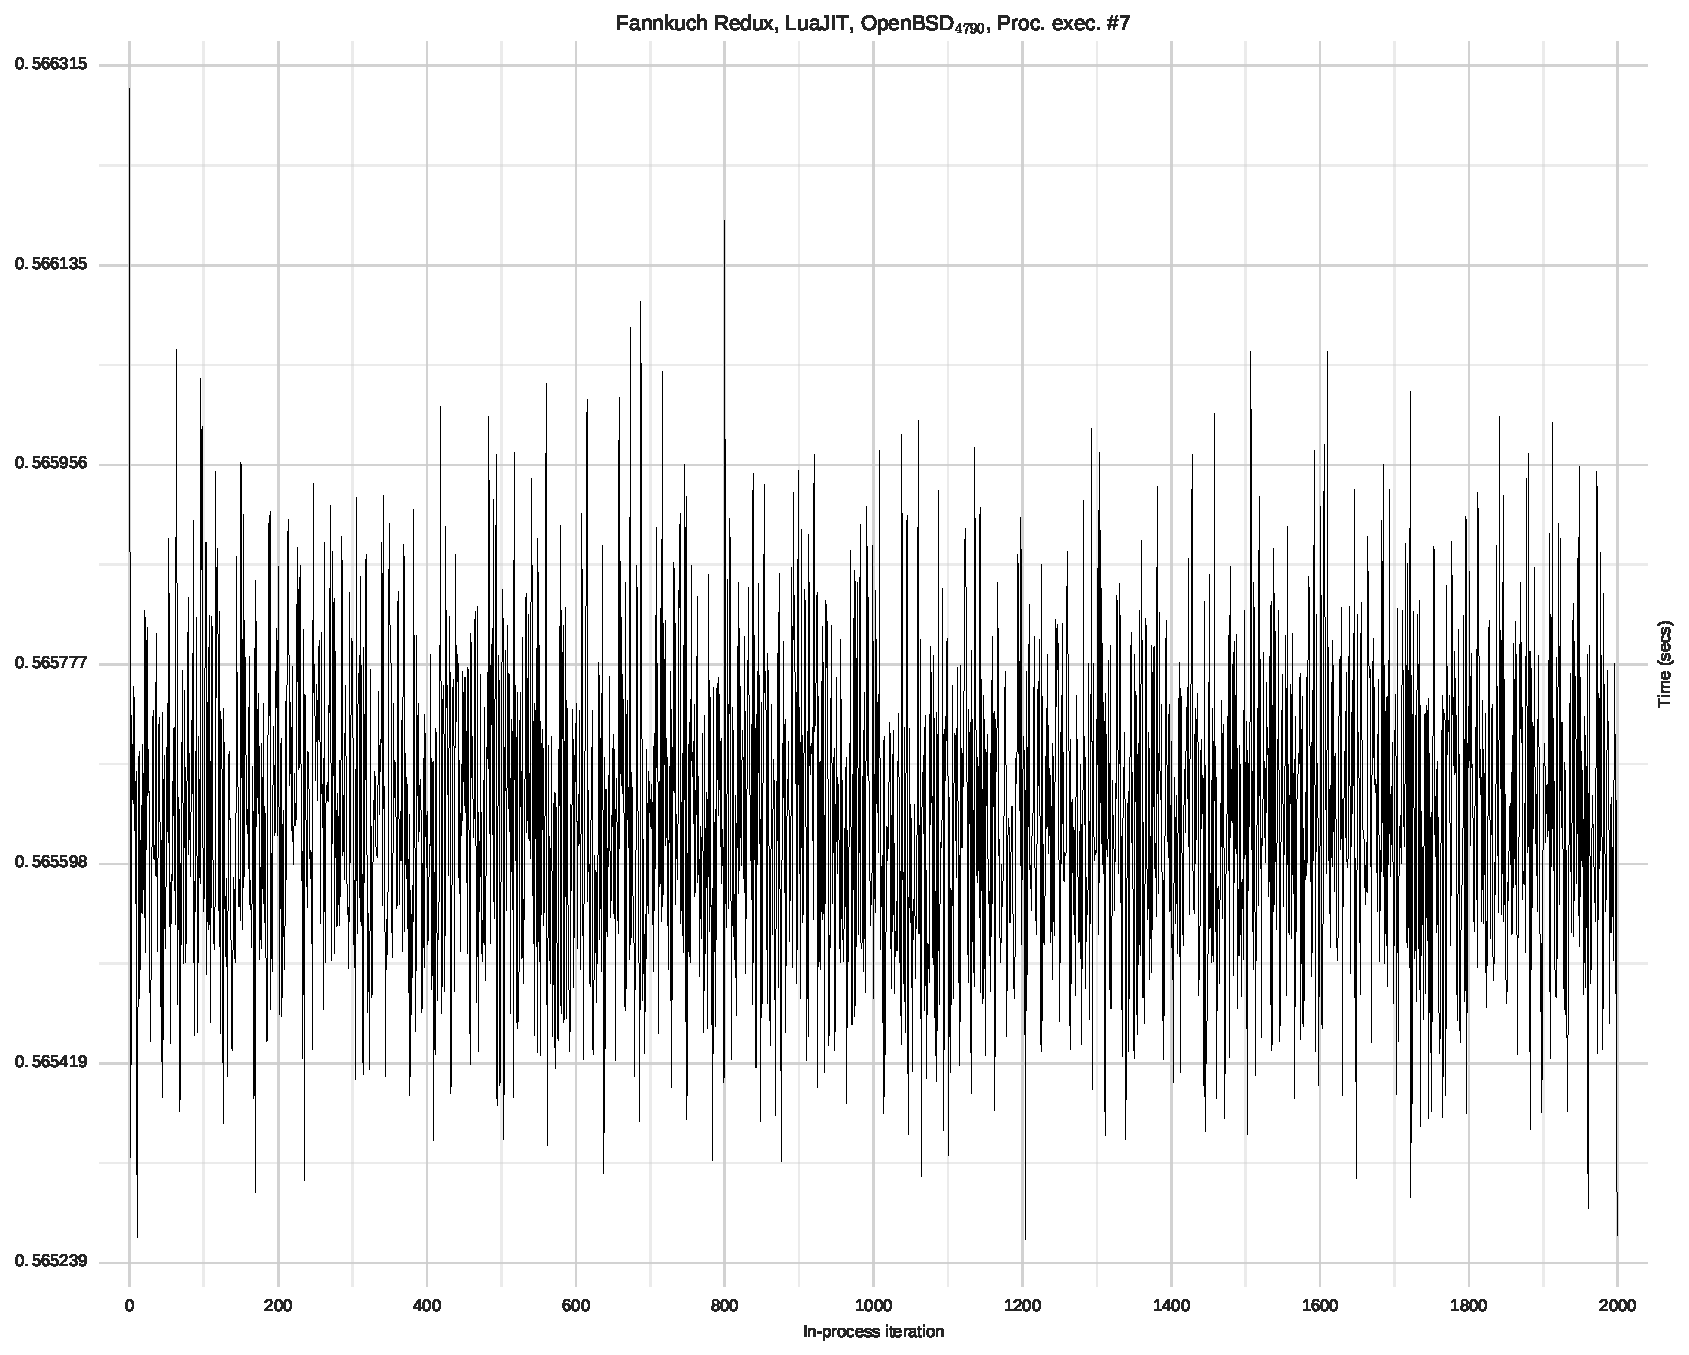
\includegraphics[width=.45\textwidth]{category_examples/flat/flat1.pdf}
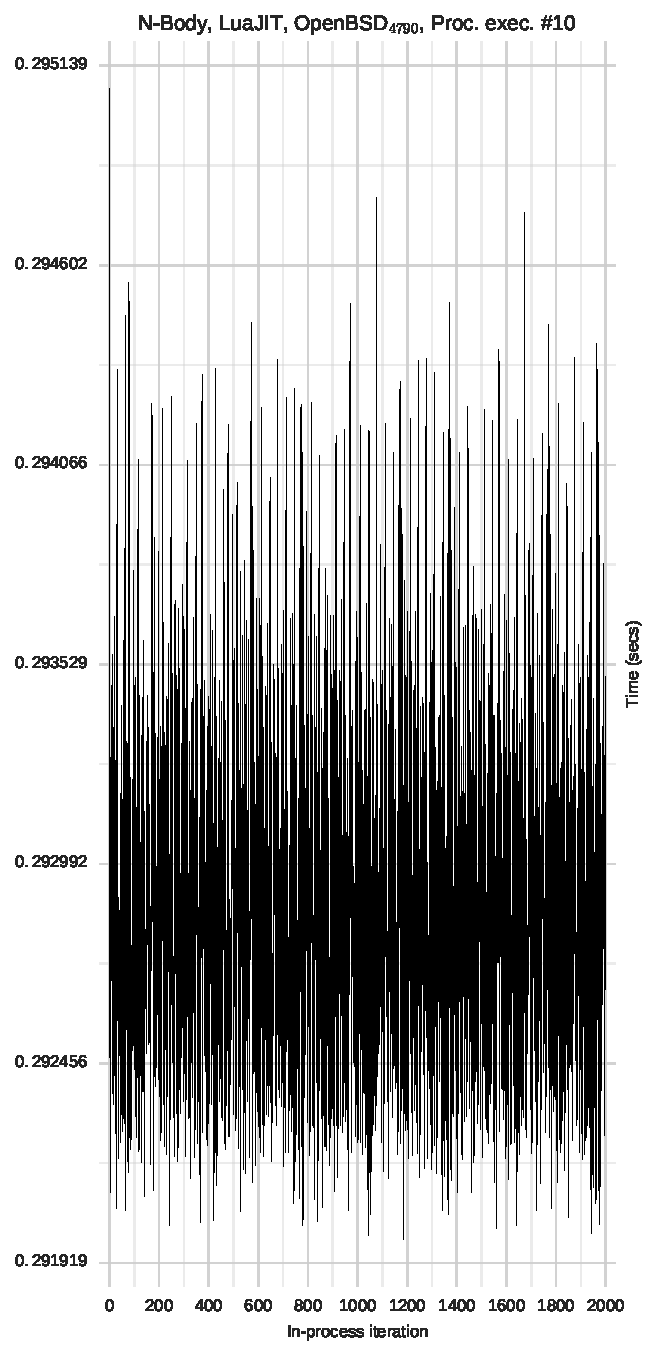
\includegraphics[width=.45\textwidth]{category_examples/flat/flat2.pdf}
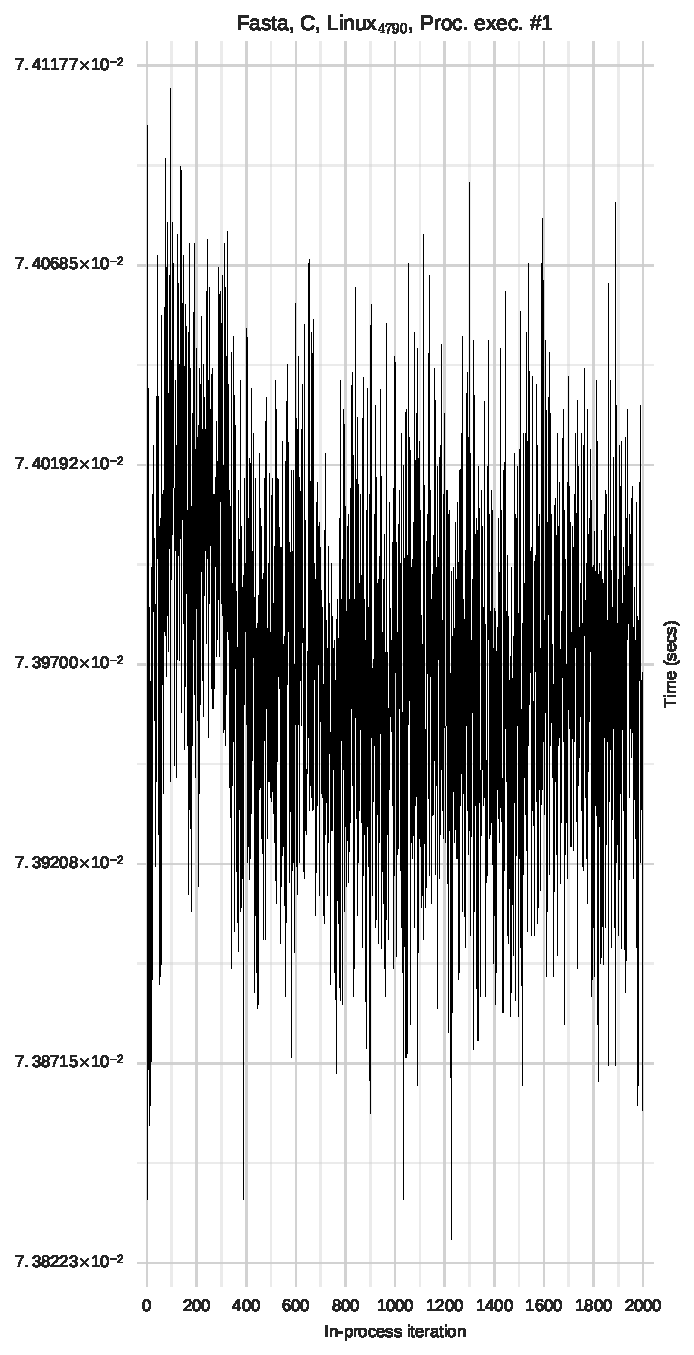
\includegraphics[width=.45\textwidth]{category_examples/flat/flat3.pdf}

\clearpage
\subsection{Examples of Slowdown Behaviour}
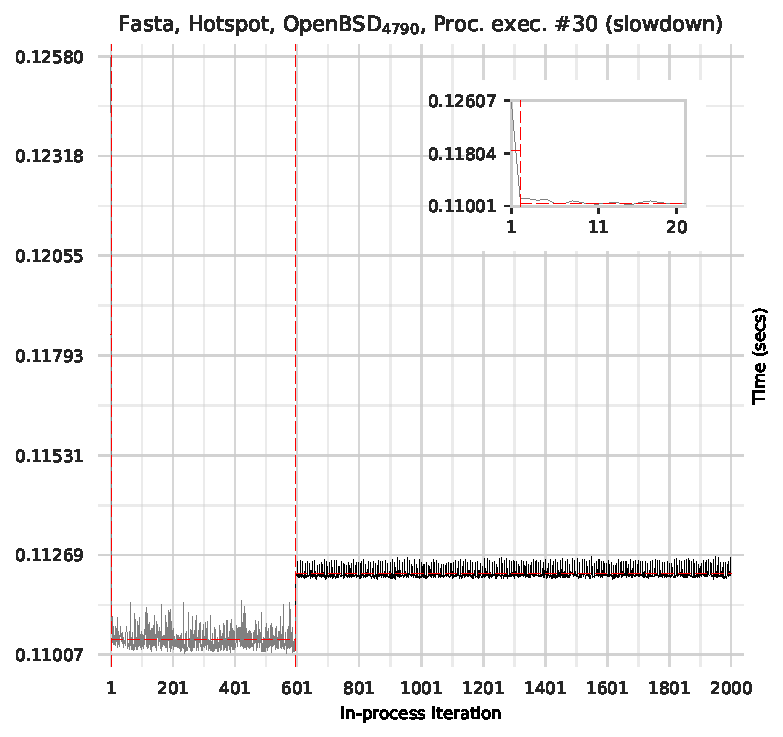
\includegraphics[width=.45\textwidth]{category_examples/slowdown/slowdown0.pdf}
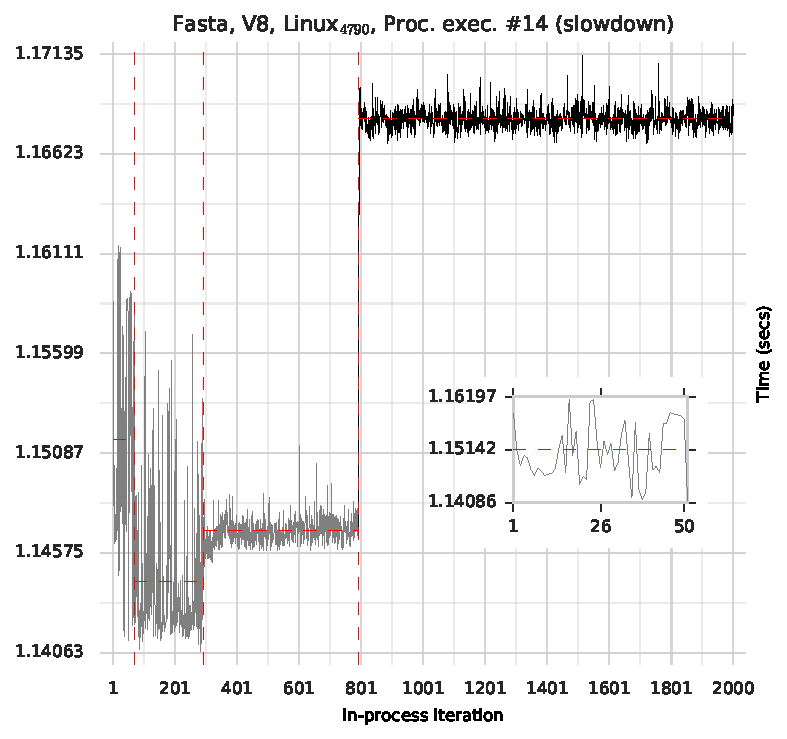
\includegraphics[width=.45\textwidth]{category_examples/slowdown/slowdown1.pdf}
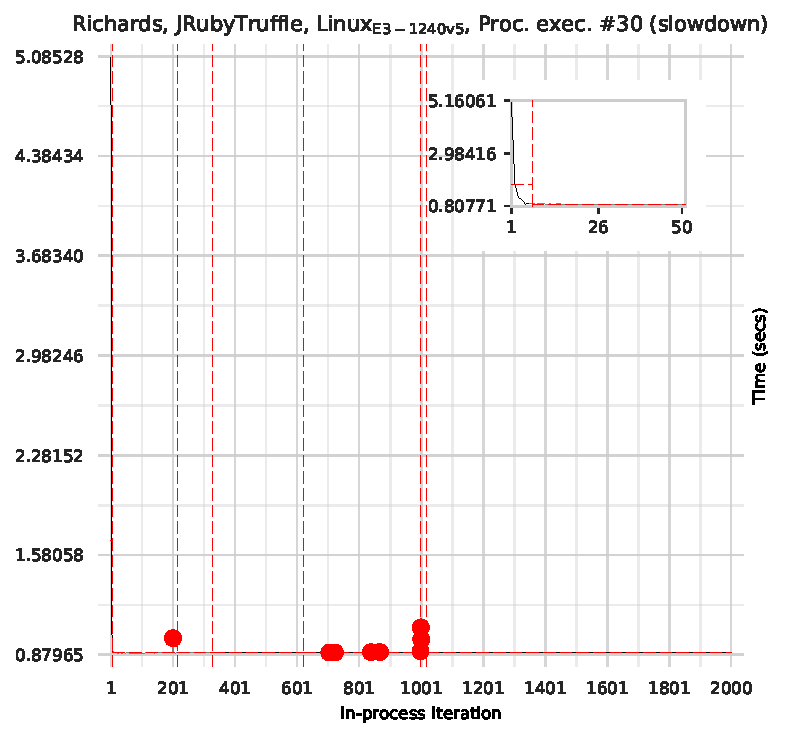
\includegraphics[width=.45\textwidth]{category_examples/slowdown/slowdown2.pdf}
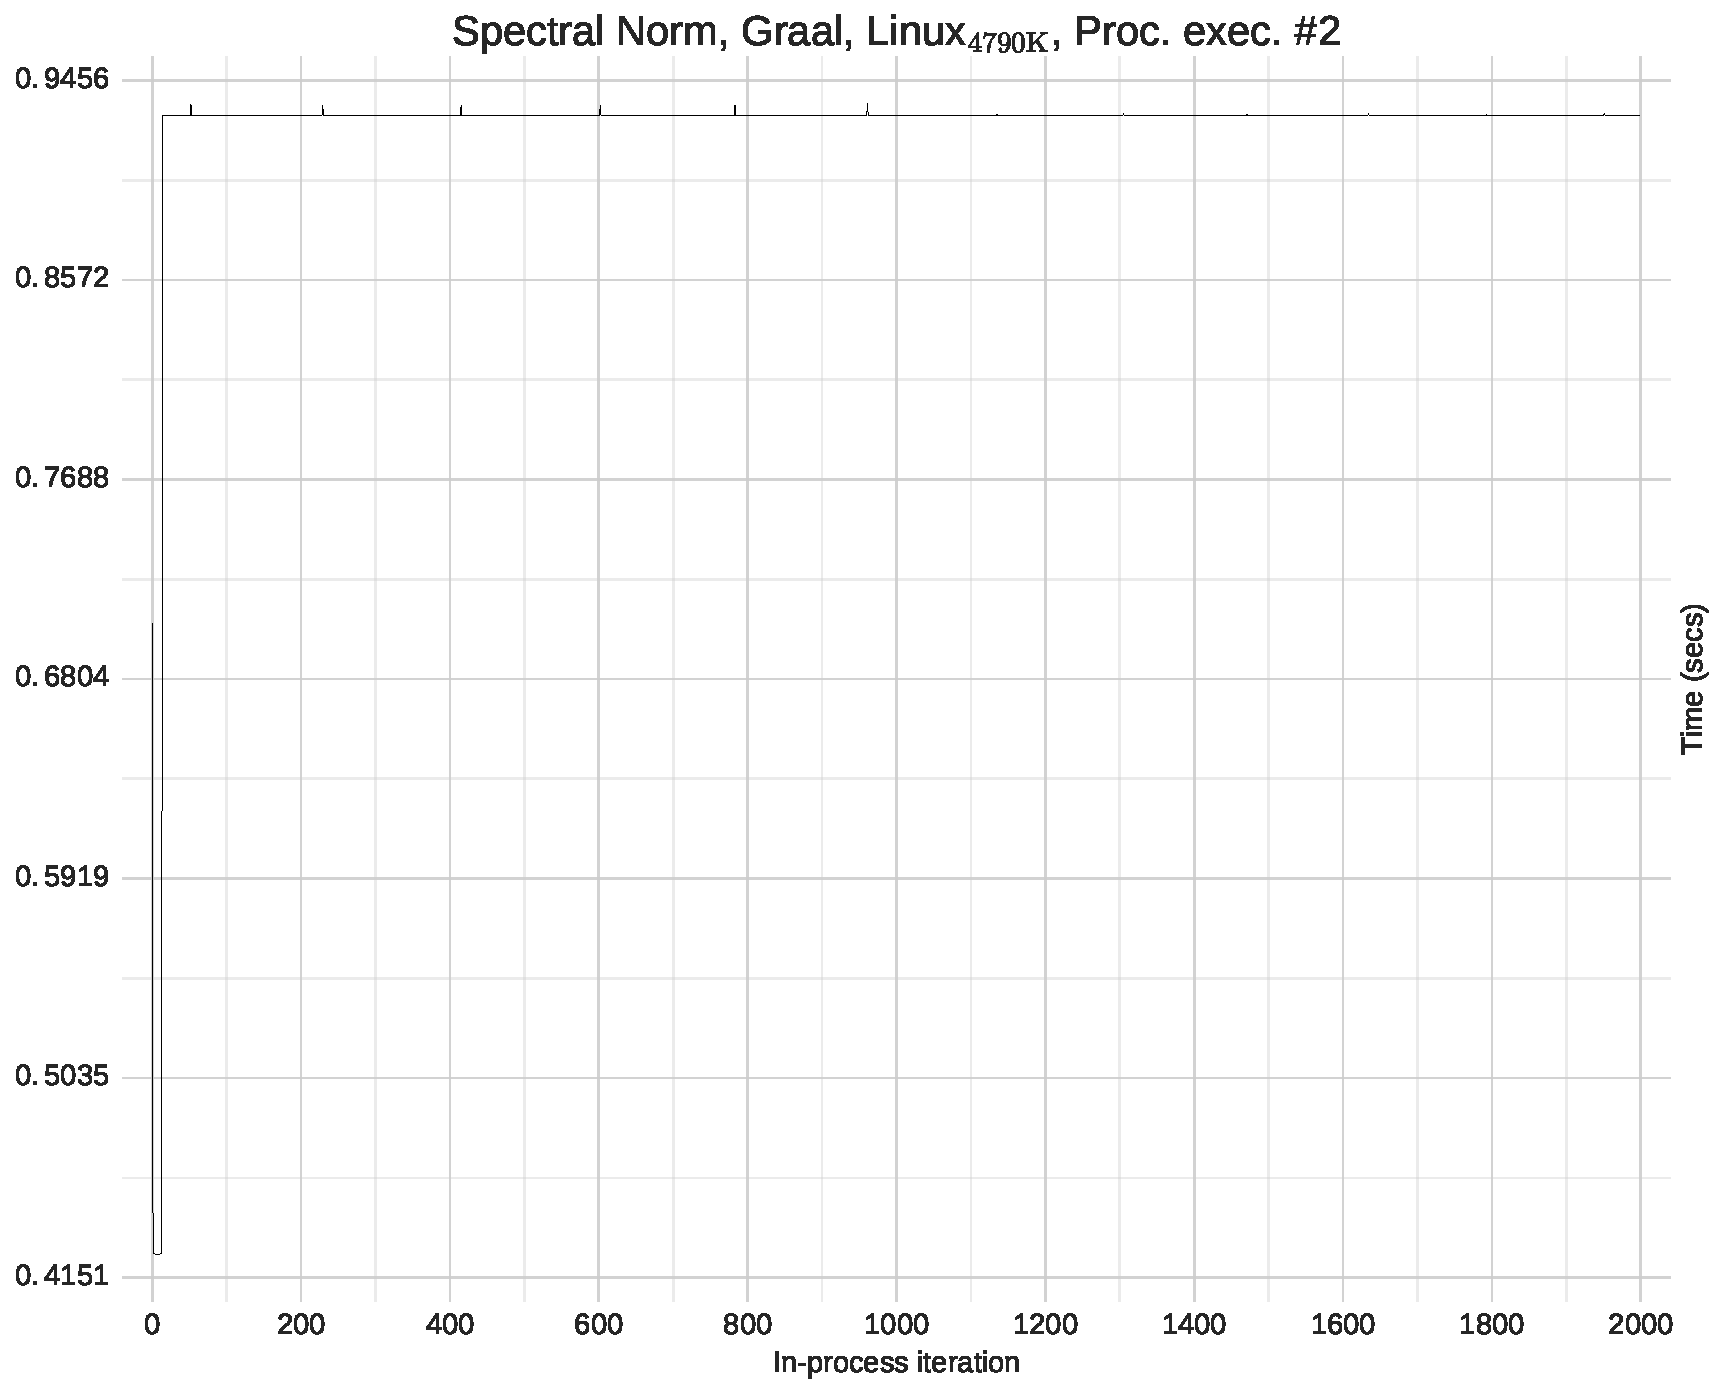
\includegraphics[width=.45\textwidth]{category_examples/slowdown/slowdown3.pdf}

\clearpage
\subsection{Examples of No Steady State Behaviour}
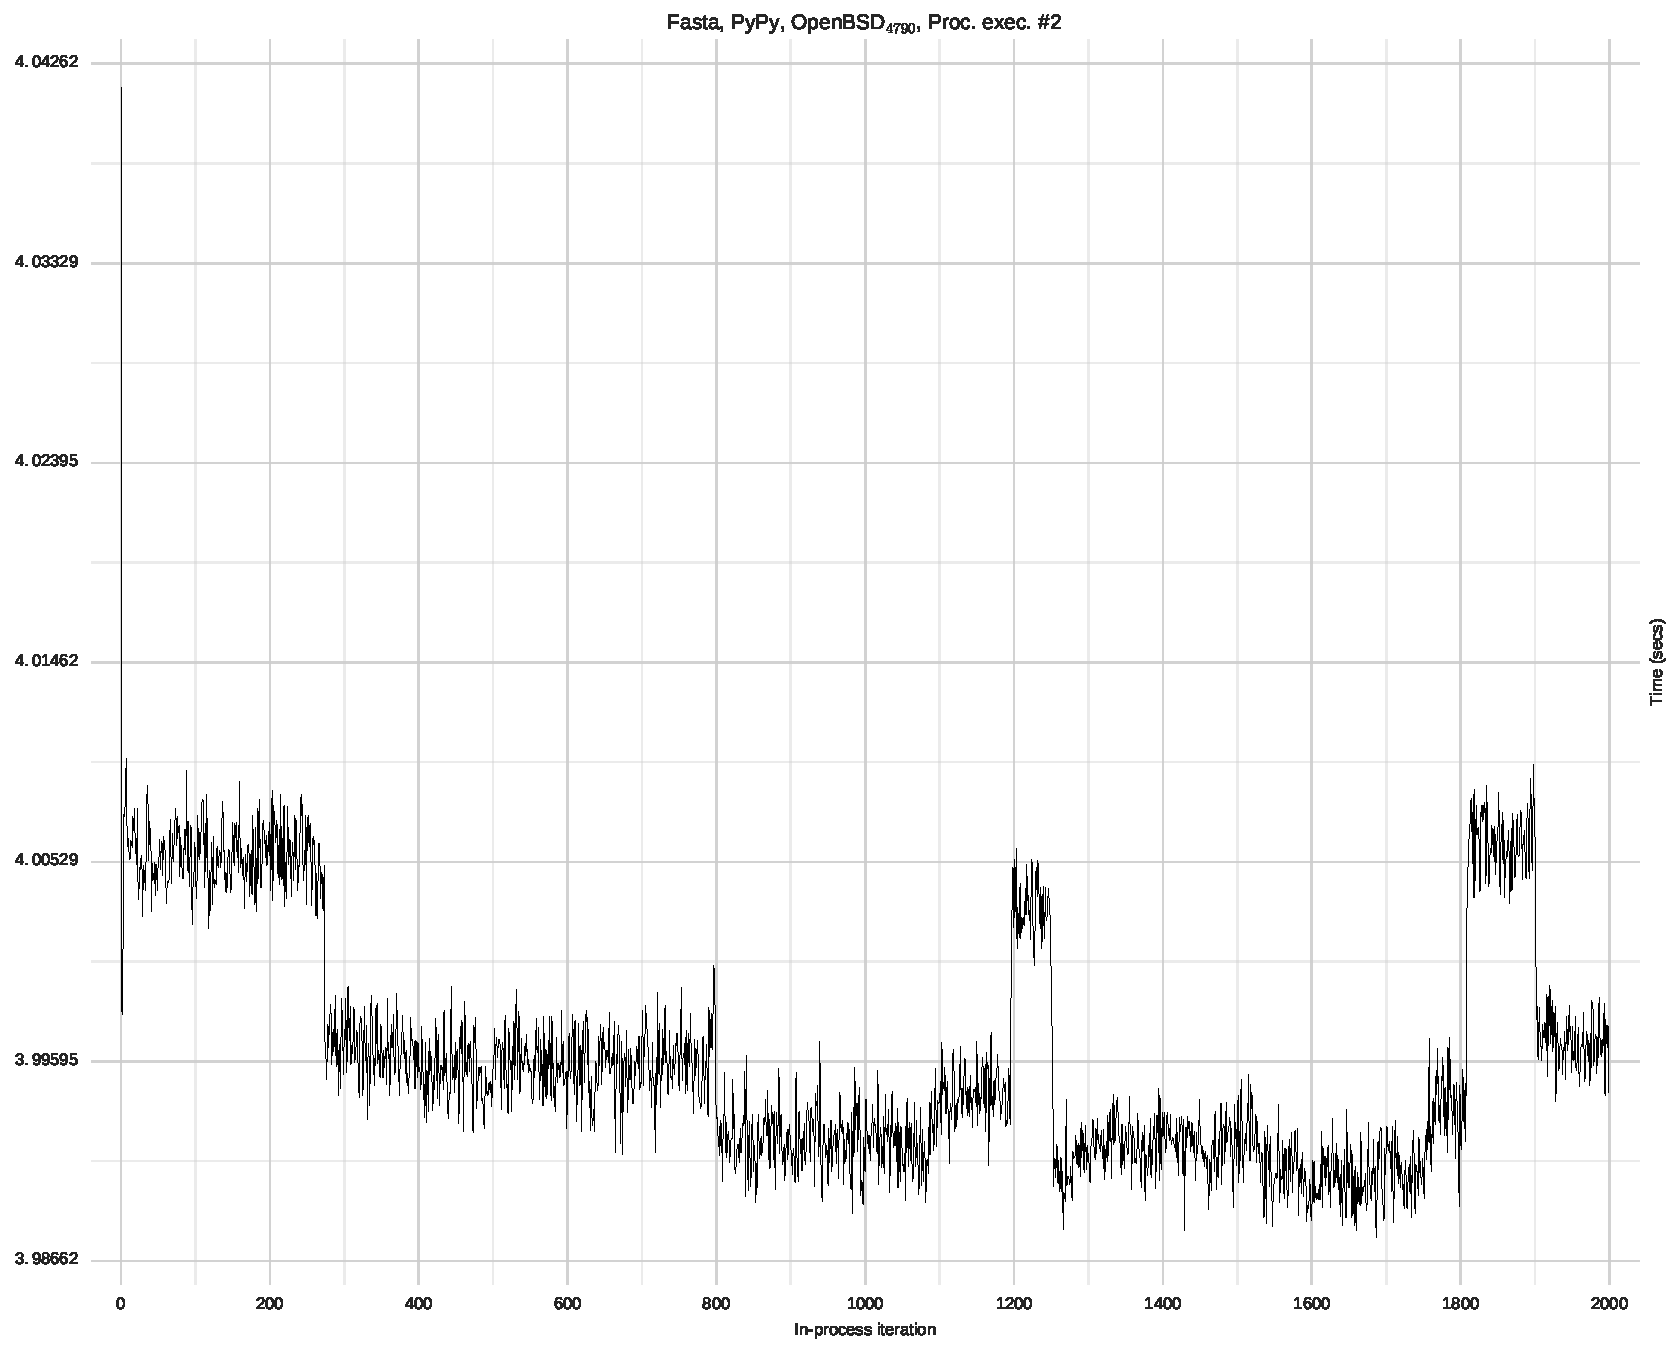
\includegraphics[width=.45\textwidth]{category_examples/nosteadystate/nosteadystate0.pdf}
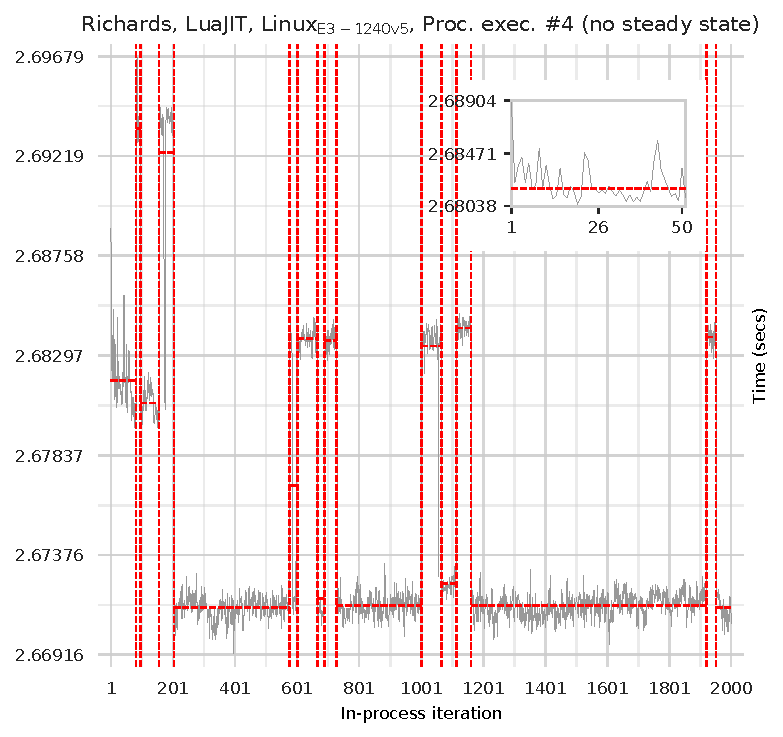
\includegraphics[width=.45\textwidth]{category_examples/nosteadystate/nosteadystate1.pdf}
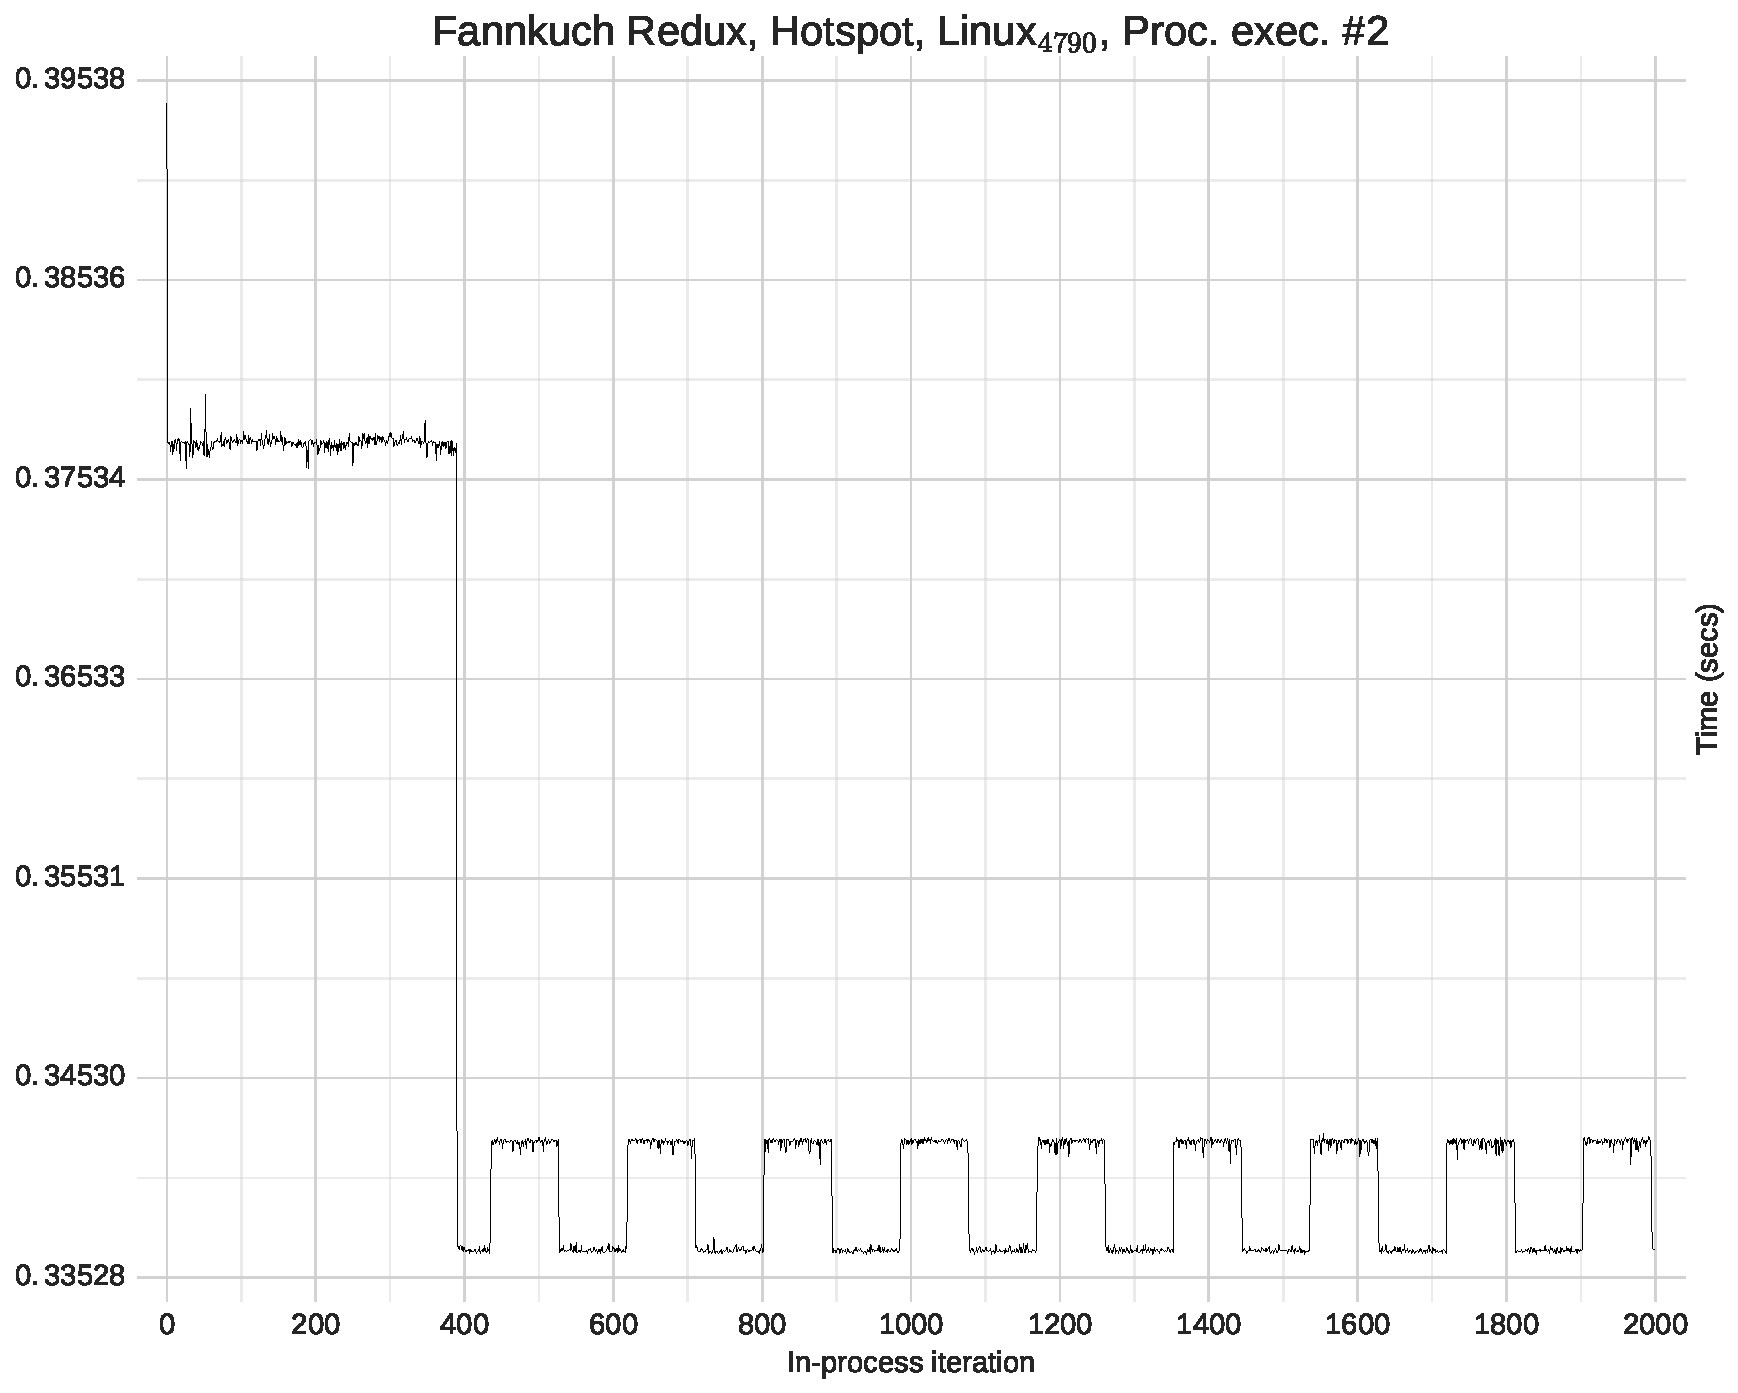
\includegraphics[width=.45\textwidth]{category_examples/nosteadystate/nosteadystate2.pdf}
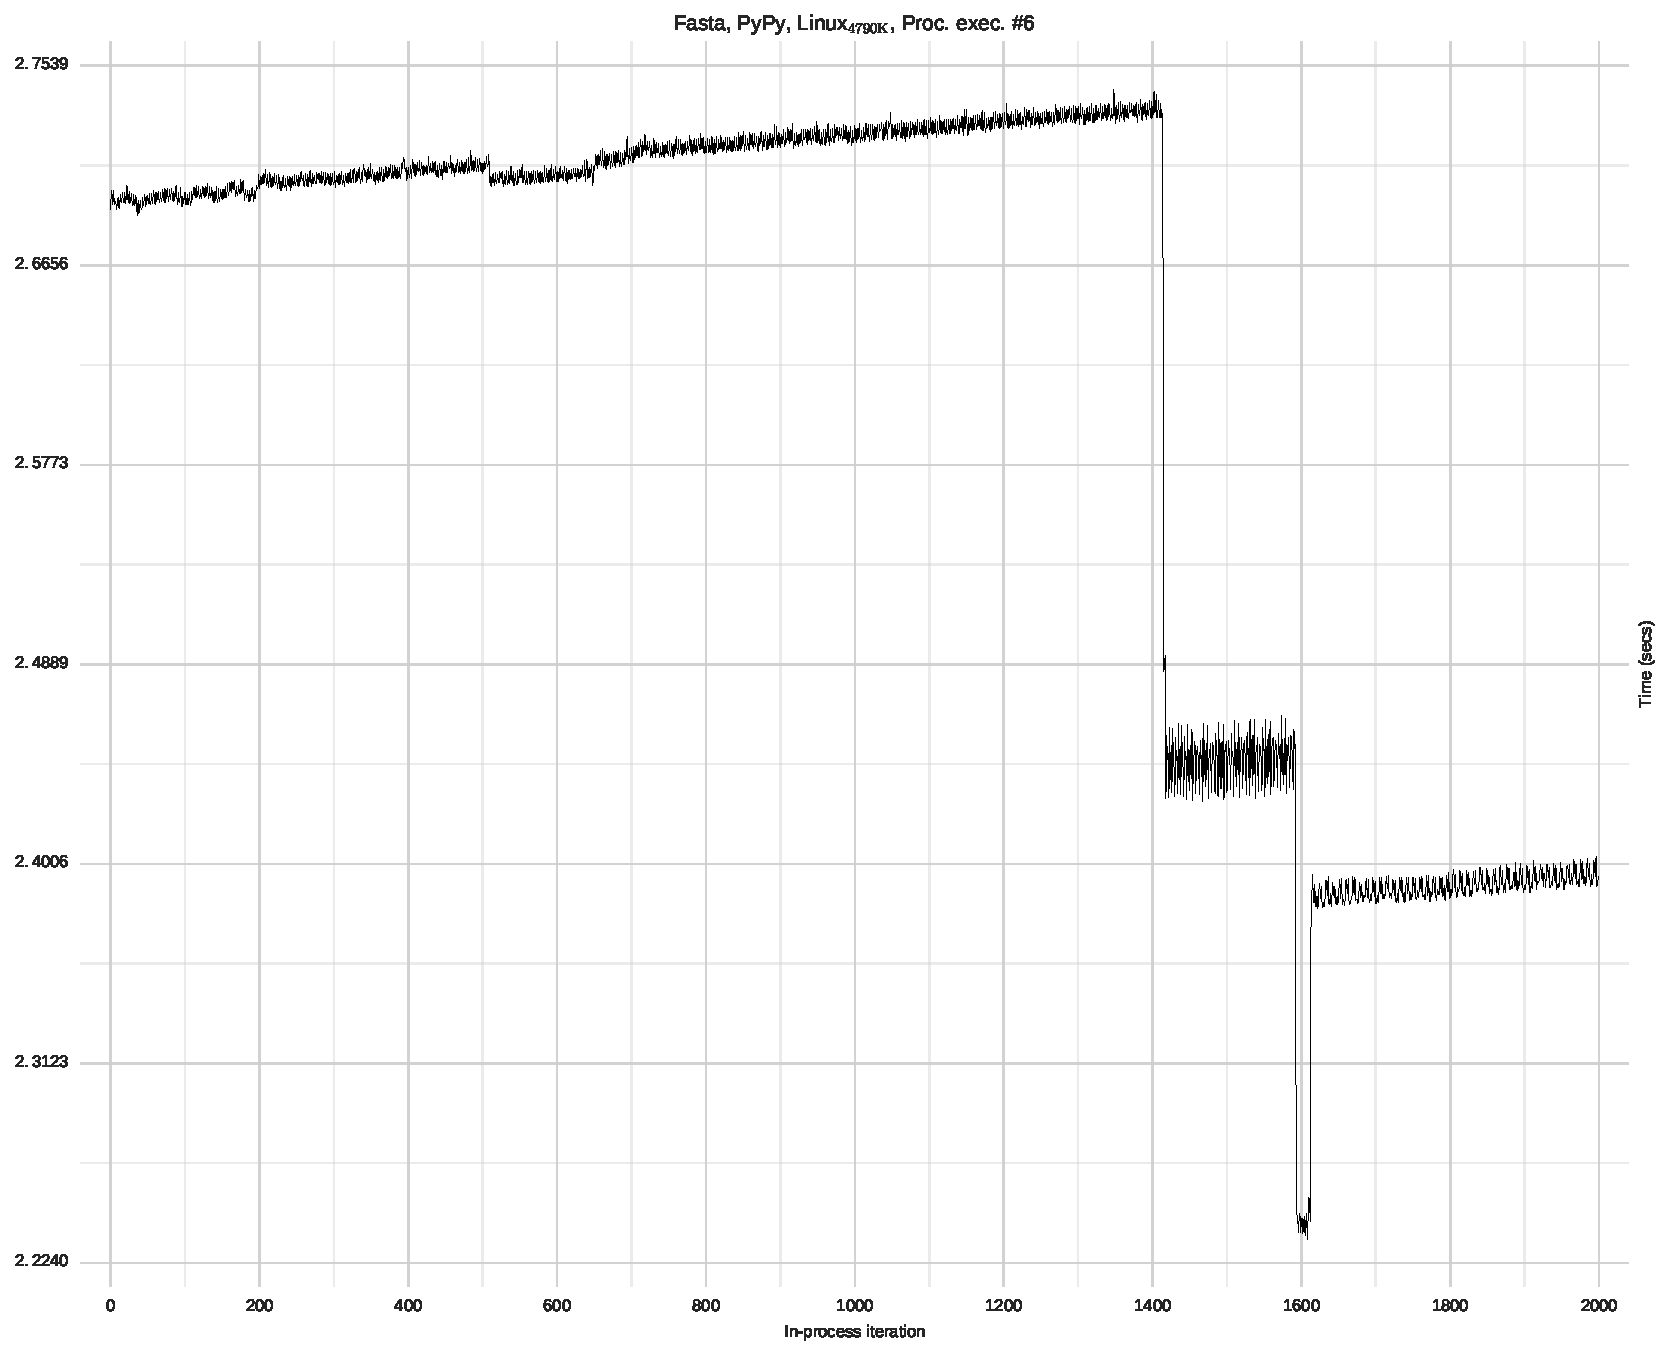
\includegraphics[width=.45\textwidth]{category_examples/nosteadystate/nosteadystate3.pdf}

\end{document}
